%% Engineering Applications of Artificial Intelligence (EAAI, Elsevier) --- elsarticle document class (two-column final layout)
\documentclass[final,5p,times,numbers]{elsarticle}

% ── Packages ────────────────────────────────────────────────────────────────
\usepackage{amssymb}
\usepackage{amsmath}
\usepackage{graphicx}
\usepackage{booktabs}
\usepackage{multirow}
\usepackage{hyperref}
\usepackage{xcolor}
\usepackage{array}
\usepackage{tabularx}
\usepackage{subcaption}
\captionsetup[figure]{labelfont=bf,labelsep=period,name={Fig.},font=footnotesize}
\captionsetup[table]{labelfont=normalfont,labelsep=period,name={Table},font=footnotesize}
\captionsetup[sub]{labelfont=normalfont,textfont=normalfont,font=footnotesize,labelformat=parens}
\usepackage{microtype}
\usepackage[capitalise]{cleveref}
\crefname{figure}{Fig.}{Figs.}
\Crefname{figure}{Fig.}{Figs.}
\crefname{table}{Table}{Tables}
\Crefname{table}{Table}{Tables}
\usepackage{textcomp}
\usepackage{rotating}
\usepackage{float}
\usepackage{algorithm}
\usepackage{algpseudocode}

% Allow line breaking at underscores in \texttt and inline text to prevent column overflows
\let\oldunderscore\_
\renewcommand{\_}{\oldunderscore\allowbreak}
\DeclareTextFontCommand{\texttt}{\ttfamily\hyphenchar\font=`\-}

% Ensure algorithm* is defined for two-column layout
\makeatletter
\@ifundefined{algorithm*}{%
  \newenvironment{algorithm*}[1][t]%
    {\@dblfloat{algorithm}[#1]}%
    {\end@dblfloat}%
}{}
\makeatother

% Robust definition of \textwarning to prevent compilation halt
\providecommand{\textwarning}{\ensuremath{\triangle}}

\graphicspath{{figures/}}

\journal{Engineering Applications of Artificial Intelligence}

% Ensure corresponding author symbol is an asterisk to avoid lowercase letter collision
\makeatletter
\def\thecorref{\ast}
% Float placement parameters for double-column layout
\setlength{\@fptop}{0pt}
\setlength{\@fpbot}{0pt plus 1fil}
\setlength{\@fpsep}{12pt plus 2pt minus 2pt}
\makeatother

\setcounter{topnumber}{4}
\setcounter{dbltopnumber}{3}
\renewcommand{\topfraction}{0.95}
\renewcommand{\bottomfraction}{0.80}
\renewcommand{\dbltopfraction}{0.95}
\renewcommand{\textfraction}{0.05}
\renewcommand{\floatpagefraction}{0.85}
\renewcommand{\dblfloatpagefraction}{0.85}

% ── Document ─────────────────────────────────────────────────────────────────
\begin{document}

\begin{frontmatter}

\title{Adaptive Multi-Horizon Electricity Procurement Using Reinforcement Learning and Macroeconomic News Sentiment}

\author[inst1]{Manel Mart{\'i}nez-Retamal}
\ead{manel.martinez@uah.es}

\author[inst2]{David Gualda}
\ead{david.gualda@urjc.es}

\author[inst1]{Reinier Herrera-Casanova}
\ead{reinier.herrera@uah.es}

\author[inst3]{Leonardo Pe\~na-Pupo}
\ead{lpepup@utu.fi}

\author[inst1]{Carlos Santos-P{\'e}rez\corref{cor1}}
\ead{carlos.santos@uah.es}
\cortext[cor1]{Corresponding author}

\affiliation[inst1]{organization={Department of Signal Processing and Communications, Universidad de Alcal{\'a}},
             addressline={Campus Universitario, Ctra. Madrid-Barcelona km 33.6},
             city={Alcal{\'a} de Henares},
             postcode={28805},
             state={Madrid},
             country={Spain}}

\affiliation[inst2]{organization={Department of Signal Theory and Communications, Telematics and Computing Systems, Universidad Rey Juan Carlos},
             addressline={Camino del Molino s/n},
             city={Fuenlabrada},
             postcode={28943},
             state={Madrid},
             country={Spain}}

\affiliation[inst3]{organization={Finland Futures Research Centre, Turku School of Economics, University of Turku},
             city={Turku},
             postcode={20014},
             country={Finland}}

% ── Abstract ─────────────────────────────────────────────────────────────────
\begin{abstract}
Industrial electricity consumers must decide when to hedge power purchases across spot and forward contracts under volatile wholesale prices. This study formulates Iberian baseload procurement as an engineering decision problem over 14 spot and forward instruments in MIBEL and develops an adaptive deep reinforcement learning (DRL) framework whose state combines physical grid fundamentals, OMIP settlement curves, and ten continuous news-sentiment dimensions extracted with a zero-shot large language model (LLM). We compare physical, commodity, sentiment, and combined representations through a controlled $2 \times 2$ ablation, then evaluate monthly rolling Walk-Forward retraining over 374 delivery days (2023--2026). The isolated early-2026 shock window contains 148 calendar delivery days (102 official OMIP trading sessions and 46 non-trading dates) with a 34.6\% mean spot-price decrease relative to 2025. The Kolmogorov--Smirnov statistic is 0.3653 (bootstrap 95\% CI: $[0.2570, 0.5265]$; empirical $p_{\text{emp}} \le 0.0002$), while demand and solar profiles show no significant marginal shifts under Bonferroni correction. The multimodal policy achieves estimated savings of $6.04\%$ across 374 Walk-Forward days and $+6.32\%$ in early 2026 ($+6.32 \pm 11.60\%$ over 44 active Walk-Forward test sessions; $+6.32\%$ across the 148-day window). A fixed two-day forward rule attains higher 2026 savings ($+11.18\%$) but also higher downside semi-deviation ($13.68$ vs $9.15$ \texteuro/MWh) and maximum drawdown ($225.45$ vs $186.45$ \texteuro/MWh). Because feature ablation uses a single seed and architecture search is post-selection, results do not establish causal sentiment effects or universal economic superiority, but demonstrate an adaptive savings--risk trade-off for industrial energy procurement.
\end{abstract}

% ── Keywords ─────────────────────────────────────────────────────────────────
\begin{keyword}
Energy procurement \sep Wholesale electricity markets \sep Deep reinforcement learning \sep Macroeconomic news sentiment \sep Concept drift \sep Walk-forward validation
\end{keyword}

\noindent\textit{INSPEC classification codes:} C1230P, C1250, C7120, C3350, C1180, C7410

\end{frontmatter}

\begin{table*}[!t]
\centering
\setlength{\fboxsep}{6pt}%
\setlength{\fboxrule}{0.5pt}%
\fbox{%
\begin{minipage}{0.98\textwidth}
\textbf{\large Nomenclature}\\[0.4em]
\begin{minipage}[t]{0.48\textwidth}
\textbf{\textit{Abbreviations}}\\[0.2em]
\scriptsize
\begin{tabularx}{\linewidth}{@{}p{1.4cm}X@{}}
\textbf{CET} & Central European Time \\
\textbf{CVaR} & Conditional Value at Risk ($95\%$) \\
\textbf{DD} & Drawdown \\
\textbf{DRL} & Deep Reinforcement Learning \\
\textbf{EU ETS} & European Union Emissions Trading System \\
\textbf{FTV / PV} & Photovoltaic Solar Generation \\
\textbf{GTrXL} & Gated Transformer-XL \\
\textbf{HPO} & Hyperparameter Optimisation \\
\textbf{KS} & Kolmogorov--Smirnov Test \\
\textbf{LLM} & Large Language Model (Llama-3 8B) \\
\textbf{LSTM} & Long Short-Term Memory Network \\
\textbf{MDP} & Markov Decision Process \\
\textbf{MIBEL} & Mercado Ib{\'e}rico de Electricidad \\
\textbf{MLP} & Multi-Layer Perceptron \\
\textbf{MTU} & Market Time Unit (1 Hour) \\
\textbf{NLP} & Natural Language Processing \\
\textbf{OMIClear} & Clearing House and Central Counterparty \\
\textbf{OMIE} & Iberian Electricity Spot Market Operator \\
\textbf{OMIP} & Iberian Electricity Derivatives Exchange \\
\textbf{OTC} & Over-the-Counter Bilateral Trading \\
\textbf{POMDP} & Partially Observable Markov Decision Process \\
\textbf{PPO} & Proximal Policy Optimization \\
\textbf{REE} & Red El{\'e}ctrica de Espa{\~n}a (Spanish TSO) \\
\textbf{RL} & Reinforcement Learning \\
\textbf{SHAP} & Shapley Additive Explanations \\
\textbf{SPOT} & Day-Ahead Spot Electricity Market \\
\textbf{TPE} & Tree-structured Parzen Estimator \\
\textbf{TSO} & Transmission System Operator \\
\textbf{TTF} & Title Transfer Facility (Natural Gas) \\
\end{tabularx}
\end{minipage}%
\hfill
\begin{minipage}[t]{0.49\textwidth}
\textbf{\textit{Variables and Parameters}}\\[0.2em]
\scriptsize
\begin{tabularx}{\linewidth}{@{}p{1.6cm}X@{}}
$t$ & Active trading day index \\
$H$ & Maximum forward delivery horizon ($H = 400$ days) \\
$a_0$ & Unhedged physical SPOT procurement action \\
$a_1, a_2, a_3$ & Daily forward contracts ($D_1, D_2, D_3$) \\
$a_4 \dots a_7$ & Weekly forward contracts ($W_1 \dots W_4$) \\
$a_8 \dots a_{13}$ & Monthly forward contracts ($M_1 \dots M_6$) \\
$P_{\text{SPOT}, t}$ & OMIE day-ahead spot clearing price [\texteuro/MWh] \\
$P_{a, t}$ & OMIP daily closing settlement price for action $a$ [\texteuro/MWh] \\
$s_t$ & Environment state tuple $(\mathbf{X}_t, \mathbf{c}_t, \mathbf{m}_t) \in \mathcal{S}$ \\
$\mathbf{o}_t$ & Policy observation vector ($\mathbf{o}_t \in \mathbb{R}^{715}$) \\
$\mathbf{c}_t, \mathbf{m}_t$ & Locked forward price vector and binary delivery mask \\
$\tilde{\mathbf{c}}_t$ & Standardized inventory vector with $-10.0$ sentinel encoding \\
$W$ & Walk-Forward rolling update window ($W \in \{1, 3, 6, 12\}$ months) \\
$B$ & Total monthly evaluation calendar blocks ($B = 41$) \\
$K$ & PPO rollout interaction steps per monthly retraining ($K = 15{,}000$) \\
$\phi_1 \dots \phi_{10}$ & Zero-shot LLM news sentiment dimensions normalized to $[-1, +1]$ \\
$E_{\text{load}, d}$ & Canonical baseload demand ($24$~MWh/day per MW capacity) \\
$\gamma$ & MDP temporal discount factor ($\gamma = 0.99$) \\
$\lambda_{\text{pen}}$ & Penalty for invalid overlapping forward execution \\
$c_{\text{ent}}$ & PPO entropy regularization coefficient \\
$\sigma_-$ & Downside semi-deviation [\texteuro/MWh] \\
$S_{\%}, S_{\text{cum}}$ & Relative percentage savings (\%) and cumulative savings [\texteuro/MWh] \\
\end{tabularx}
\end{minipage}
\vspace{0.2em}
\end{minipage}%
}
\vspace{-0.5em}
\end{table*}

%% ── Main Text ────────────────────────────────────────────────────────────────
% ── Section 1: Introduction ───────────────────────────────────────────────────
\section{Introduction}
\label{sec:introduction}

The accelerating integration of variable renewable energy sources into European
wholesale electricity markets has introduced unprecedented price volatility,
reshaping the financial exposure of large-scale energy consumers.
In liberalised electricity markets, such as the Iberian market (MIBEL, comprising the Spanish and Portuguese wholesale bidding zones), wholesale 
prices (SPOT) are determined daily based on short-term supply and demand matching. 
For energy-intensive industries procuring electricity at scale, daily exposure to 
these SPOT market fluctuations can lead to substantial financial volatility, with annual 
costs swinging by tens of millions of euros.
To mitigate this exposure, large consumers rely on \textit{forward hedging}: locking 
in energy prices at fixed rates through futures contracts traded on exchanges such as 
OMIP (\textit{Operador del Mercado Ib{\'e}rico de Energ{\'i}a --- Polo Portugu{\^e}s}). By purchasing energy days, weeks, or 
months in advance, consumers secure price certainty. However, determining \textit{when} 
to purchase which contract and at which forward horizon constitutes a highly complex, 
sequential decision-making problem under deep uncertainty. Large industrial consumers operate at the intersection of physical spot clearing (OMIE, \textit{Operador del Mercado Ib\'erico de Energ\'ia --- Polo Espa\~nol}) and derivative hedging markets (OMIP), requiring multi-horizon decision-making under non-stationary market conditions (as detailed in Section~\ref{sec:methodology}).

Electricity price forecasting studies have consistently identified strong nonlinearities, spikes, seasonality and dependence on physical and market-coupling variables \cite{weron2014electricity, li2021dayahead}.
Understanding the structural drivers of SPOT prices is a prerequisite for any 
robust procurement strategy. In the Spanish market, machine-learning models using system fundamentals have been shown to provide both predictive and explanatory information about day-ahead price formation \cite{diaz2019prediction}. 
Recent peer-reviewed work in \textit{Engineering Applications of Artificial Intelligence} has also investigated decomposition-based hybrid deep-learning architectures for day-ahead electricity-price forecasting using real market data \cite{aksu2026dayahead}. Such work focuses on improving forecast accuracy; the present study instead evaluates the economic consequences of sequential procurement actions across several delivery horizons, under settlement and inventory constraints. 
More broadly, the forecasting literature stresses that predictive accuracy does not automatically translate into optimal procurement decisions under risk and contractual constraints \cite{weron2014electricity, hanetho2023commodities}.

This distinction has encouraged the use of reinforcement learning, which optimises a sequential decision policy directly against a specified reward function rather than against forecast error alone~\cite{sutton2018reinforcement}.
The financial exposure of consumers to wholesale volatility has sparked a growing 
body of DRL research. A comprehensive review of reinforcement learning in deregulated energy markets shows that existing applications concentrate mainly on bidding, dispatch, demand response and storage operation \cite{zhu2023reinforcement, ochoa2022multiagent}. For instance, recent work in \textit{Engineering Applications of Artificial Intelligence} has applied deep reinforcement learning to producer-side strategic bidding, explicitly modelling competitor behaviour and multi-dimensional price--quantity offers \cite{hu2025strategicbidding}. This is a closely related market-decision problem, but differs from the consumer-side task studied here: allocating baseload purchases across spot and forward-delivery instruments rather than optimizing a producer's market offers. Consumer-side procurement through multiple forward delivery horizons and explicit inventory constraints remains comparatively less explored. For instance, \cite{ding2025risk} proposed a risk-aware RL 
algorithm for data centre energy management that minimises costs by deferring 
computational workloads away from peak-price periods. While effective, this approach 
optimises internal operations rather than the financial procurement instrument itself.
Focusing directly on financial trading, \cite{hanetho2023commodities} showed that 
Deep Policy Gradient methods employing LSTM architectures generate superior Sharpe 
ratios compared to passive buy-and-hold strategies when trading natural gas futures.
To address the inherent sensitivity of DRL policies to distribution shifts, 
\cite{qiu2025robust} proposed an adversarial robust RL framework for electricity 
market bidding, defining an explicit uncertainty set around state transitions.
Additionally, at the intersection of Natural Language Processing, Large Language Models (LLMs), and energy market analysis, several distinct research directions have emerged. In commodity derivative markets, Cui et al.~\cite{cui2025toward} proposed integrating LLM-derived macroeconomic sentiment and market connectedness as exogenous state variables for speculative futures trading in crude oil, while Hanetho and Fleten~\cite{hanetho2023commodities} explored recurrent deep policy networks on natural gas futures without textual signals. In power systems, Chen et al.~\cite{chen2025modeling} developed an emotion-semantic representation paired with reinforcement learning for multi-objective virtual power plant (VPP) operational bidding and revenue optimization. Parallel forecasting studies, such as Wang and Yu~\cite{wang2025electricity} using TimeXer neural forecasters with LLM sentiment on CAISO, Zhang et al.~\cite{tempr2025llm} deploying LLM bidding and market sentiment agents for electricity price and spike prediction, and Manowska and Hassan~\cite{manowska2026modeling} evaluating news indicators for Polish electricity price formation, demonstrate that textual sentiment contains leading signals for power market dynamics.

Two recent studies in \textit{Engineering Applications of Artificial Intelligence} are particularly relevant to the text--market interface. Liu and Qin~\cite{liu2026scaleaware} fuse news and policy text with numerical market variables for scale-aware carbon-price forecasting, while Kang et al.~\cite{kang2026structuredsentiment} use LLM-derived, supply-chain-specific sentiment from public energy, regulatory and corporate documents to forecast crude-oil prices and evaluate its predictive and trading value. These studies show that textual information and numerical market data are already being combined for energy-related price analysis; therefore, the present work does not claim novelty from using news sentiment or multimodal inputs alone. Its narrower contribution is to test the incremental value of such features inside a sequential industrial-consumer procurement policy over spot and multiple forward-delivery instruments, using chronological Walk-Forward evaluation and explicit savings--downside-risk comparisons.

Procurement-oriented reinforcement learning has also been investigated in a closely related setting. Wang et al.~\cite{wang2026procurement} develop a multi-market agency-procurement framework for Chinese power-grid companies, coupling multidimensional risk quantification with an A3C purchasing agent. This work confirms that procurement-cost and risk optimisation with reinforcement learning is an established research direction. The distinction addressed here is narrower: consumer-side baseload commitments in the Iberian market, allocation across 14 spot and OMIP forward-delivery instruments, and an explicit test of whether zero-shot LLM-derived news dimensions add information beyond physical and commodity inputs under chronological evaluation. These differences define the scope of the present contribution; they do not imply that procurement with reinforcement learning or the use of sentiment in energy markets is novel in itself. Table~\ref{tab:literature_comparison} provides a structured comparison with the closest related studies in the literature.

\begin{table*}[!t]
\centering
\footnotesize
\setlength{\tabcolsep}{3.0pt}
\caption{Comparison of the proposed framework with related studies combining reinforcement learning, machine learning, and textual sentiment in energy markets.}
\label{tab:literature_comparison}
\begin{tabularx}{\textwidth}{@{}l >{\hsize=0.85\hsize\raggedright\arraybackslash}X >{\hsize=1.05\hsize\raggedright\arraybackslash}X >{\hsize=0.95\hsize\raggedright\arraybackslash}X >{\hsize=0.95\hsize\raggedright\arraybackslash}X >{\hsize=1.00\hsize\raggedright\arraybackslash}X >{\hsize=1.20\hsize\raggedright\arraybackslash}X@{}}
\toprule
\textbf{Study} & \textbf{Market} & \textbf{Decision Scope / Task} & \textbf{Instruments} & \textbf{Model / Architecture} & \textbf{Text / Sentiment Signal} & \textbf{Evaluation \& Validation} \\
\midrule
Hanetho et al.~\cite{hanetho2023commodities} & UK/EU Gas & Speculative financial trading & Single futures contract & Recurrent RL (LSTM) & None & Rolling train/test (Lagged settlement) \\
Cui et al.~\cite{cui2025toward} & WTI Crude Oil & Speculative futures trading & Continuous futures & Feed-Forward DRL & Zero-shot LLM (Daily macro news) & Static train/test partition \\
Chen et al.~\cite{chen2025modeling} & Virtual Power Plant & Multi-objective dispatch / revenue & VPP internal dispatch & DRL with emotion-semantic & News sentiment analysis & Multi-objective operational simulation \\
Wang \& Yu~\cite{wang2025electricity} & US Power (CAISO) & Price forecasting (RMSE/MAE) & Day-ahead pool price & TimeXer neural forecaster & LLM-based sentiment series & Out-of-sample forecast benchmarking \\
Zhang et al.~\cite{tempr2025llm} & Power Market & Price / spike prediction & Spot price spikes & LLM bidding / sentiment agents & Multi-agent market sentiment & Out-of-sample prediction testing \\
Manowska \& Hassan~\cite{manowska2026modeling} & Poland Power & Price formation econometrics & Day-ahead wholesale & Econometric / ML regression & Textual news sentiment & Chronological out-of-sample testing \\
Wang et al.~\cite{wang2026procurement} & China Grid & Agency power procurement & Multi-market electricity & A3C purchasing agent & Public opinion risk (non-LLM) & Static empirical simulation \\
Hu et al.~\cite{hu2025strategicbidding} & Power Market & Producer-side strategic bidding & Price--quantity offers & VAE--DBSCAN and imitation DRL & None & Competitor behaviour modelling \\
Aksu et al.~\cite{aksu2026dayahead} & Denmark (DK1) & Day-ahead price forecasting & Wholesale electricity & EMD/VMD, GRU/LSTM, Bayes.\ Opt. & None & Real-market forecasting benchmark \\
Liu \& Qin~\cite{liu2026scaleaware} & China ETS & Carbon-price forecasting & Carbon spot prices & Scale decomposition, BiLSTM & News sentiment \& policy semantics & Hubei/Guangzhou ETS ablation \\
Kang et al.~\cite{kang2026structuredsentiment} & Crude Oil (WTI) & Price forecasting \& trading & Spot / futures prices & ML with LLM-derived sentiment & Energy, regulatory \& corporate sentiment & Supply-chain sentiment \& trading metrics \\
\textbf{This Study} & Iberian Power (MIBEL) & Industrial consumer procurement & 14 Forward/Spot ($D_1$--$M_6$) & RecurrentPPO / GTrXL & Zero-shot LLM (10-dim macro) & Multi-seed Walk-Forward (Strict $t-1$ lag) \\
\bottomrule
\end{tabularx}
\end{table*}

The empirical question is whether news-derived sentiment adds information beyond physical fundamentals and numerical commodity variables, and whether any such information translates into an economically meaningful savings--risk trade-off under chronological evaluation. We address this question using a controlled feature-ablation design, econometric tests of conditional predictive content, rolling Walk-Forward evaluation, and comparisons with systematic forward-purchasing and partial-hedging baselines. We interpret the results as evidence about the evaluated Iberian market sample rather than as proof of a causal sentiment mechanism or universal robustness to regime changes.

To address these challenges, this study develops and evaluates an adaptive reinforcement learning framework for sequential electricity procurement that integrates physical grid fundamentals, derivative quotations, and macroeconomic news sentiment. This study makes three bounded contributions:
\begin{enumerate}
    \item \textbf{Consumer-Side Multi-Horizon Procurement Formulation under Operational Delivery Constraints:} We formulate consumer-side electricity procurement as a sequential allocation problem across 14 spot and OMIP forward instruments ($D_1$--$M_6$), with delivery commitments, single-instrument physical settlement constraints, and cash flows represented explicitly in the decision environment.
    \item \textbf{Econometric and Factorial Evaluation of Macroeconomic News Sentiment:} We evaluate the incremental predictive and decision value of news-derived macroeconomic sentiment relative to physical-system and quantitative commodity inputs, combining econometric tests of conditional predictive content (nested $F$-tests with HAC standard errors and Toda--Yamamoto Granger causality) with a controlled $2 \times 2$ factorial feature ablation.
    \item \textbf{Longitudinal Retraining and Tail-Risk Benchmarking under Market Dislocation:} We compare dynamically re-trained procurement policies (evaluating feedforward, recurrent, and self-attention architectures across a multi-year Walk-Forward protocol) with single-contract forward heuristics and the industrial partial-hedging continuum ($\alpha \cdot D_2 + (1-\alpha) \cdot \text{SPOT}$) under an observed 2026 price-dislocation episode, reporting both simulated savings point estimates, paired bootstrap confidence intervals, and downside-risk measures ($\sigma_-$, Max DD, CVaR).
\end{enumerate}
The contribution is therefore an empirical assessment of information value and risk--return trade-offs in a specific procurement setting; it does not assume that multimodal inputs necessarily outperform simpler baselines.

The remainder of this paper is organised as follows.
\Cref{sec:methodology} details the proposed methodology, including the MDP formulation, 
the LLM sentiment pipeline, and the RecurrentPPO agent.
\Cref{sec:data_analysis} presents the dataset characterisation and statistical
marginal distributional shift validation.
\Cref{sec:results} reports the experimental results of the evaluated policies under both stable 
and shock market conditions.
\Cref{sec:discussion} discusses implications, limitations, and the interpretability 
of learned policy decisions. Finally, \Cref{sec:conclusion} concludes the paper.

% ── Section 3: Methodology ────────────────────────────────────────────────────
\section{Methodology}
\label{sec:methodology}

This section outlines the mathematical and computational architecture of the proposed adaptive procurement framework. We begin by detailing the logical workflow of the four-stage pipeline, followed by the causal data ingestion protocol, the formal Markov Decision Process (MDP) formulation, the baseline decision heuristics, and the Walk-Forward rolling retraining methodology. In this setting, the agent purchases structured electricity derivative blocks (from day-ahead to multi-month maturities) listed on OMIP, modelled as financially-settled futures that hedge financial exposure against spot price volatility while daily margin tracking and mark-to-market settlements are resolved based on official exchange prices.

\subsection{Logical Flow of the Proposed Framework}
\label{subsec:logical_flow}

\begin{figure*}[!t]
    \centering
    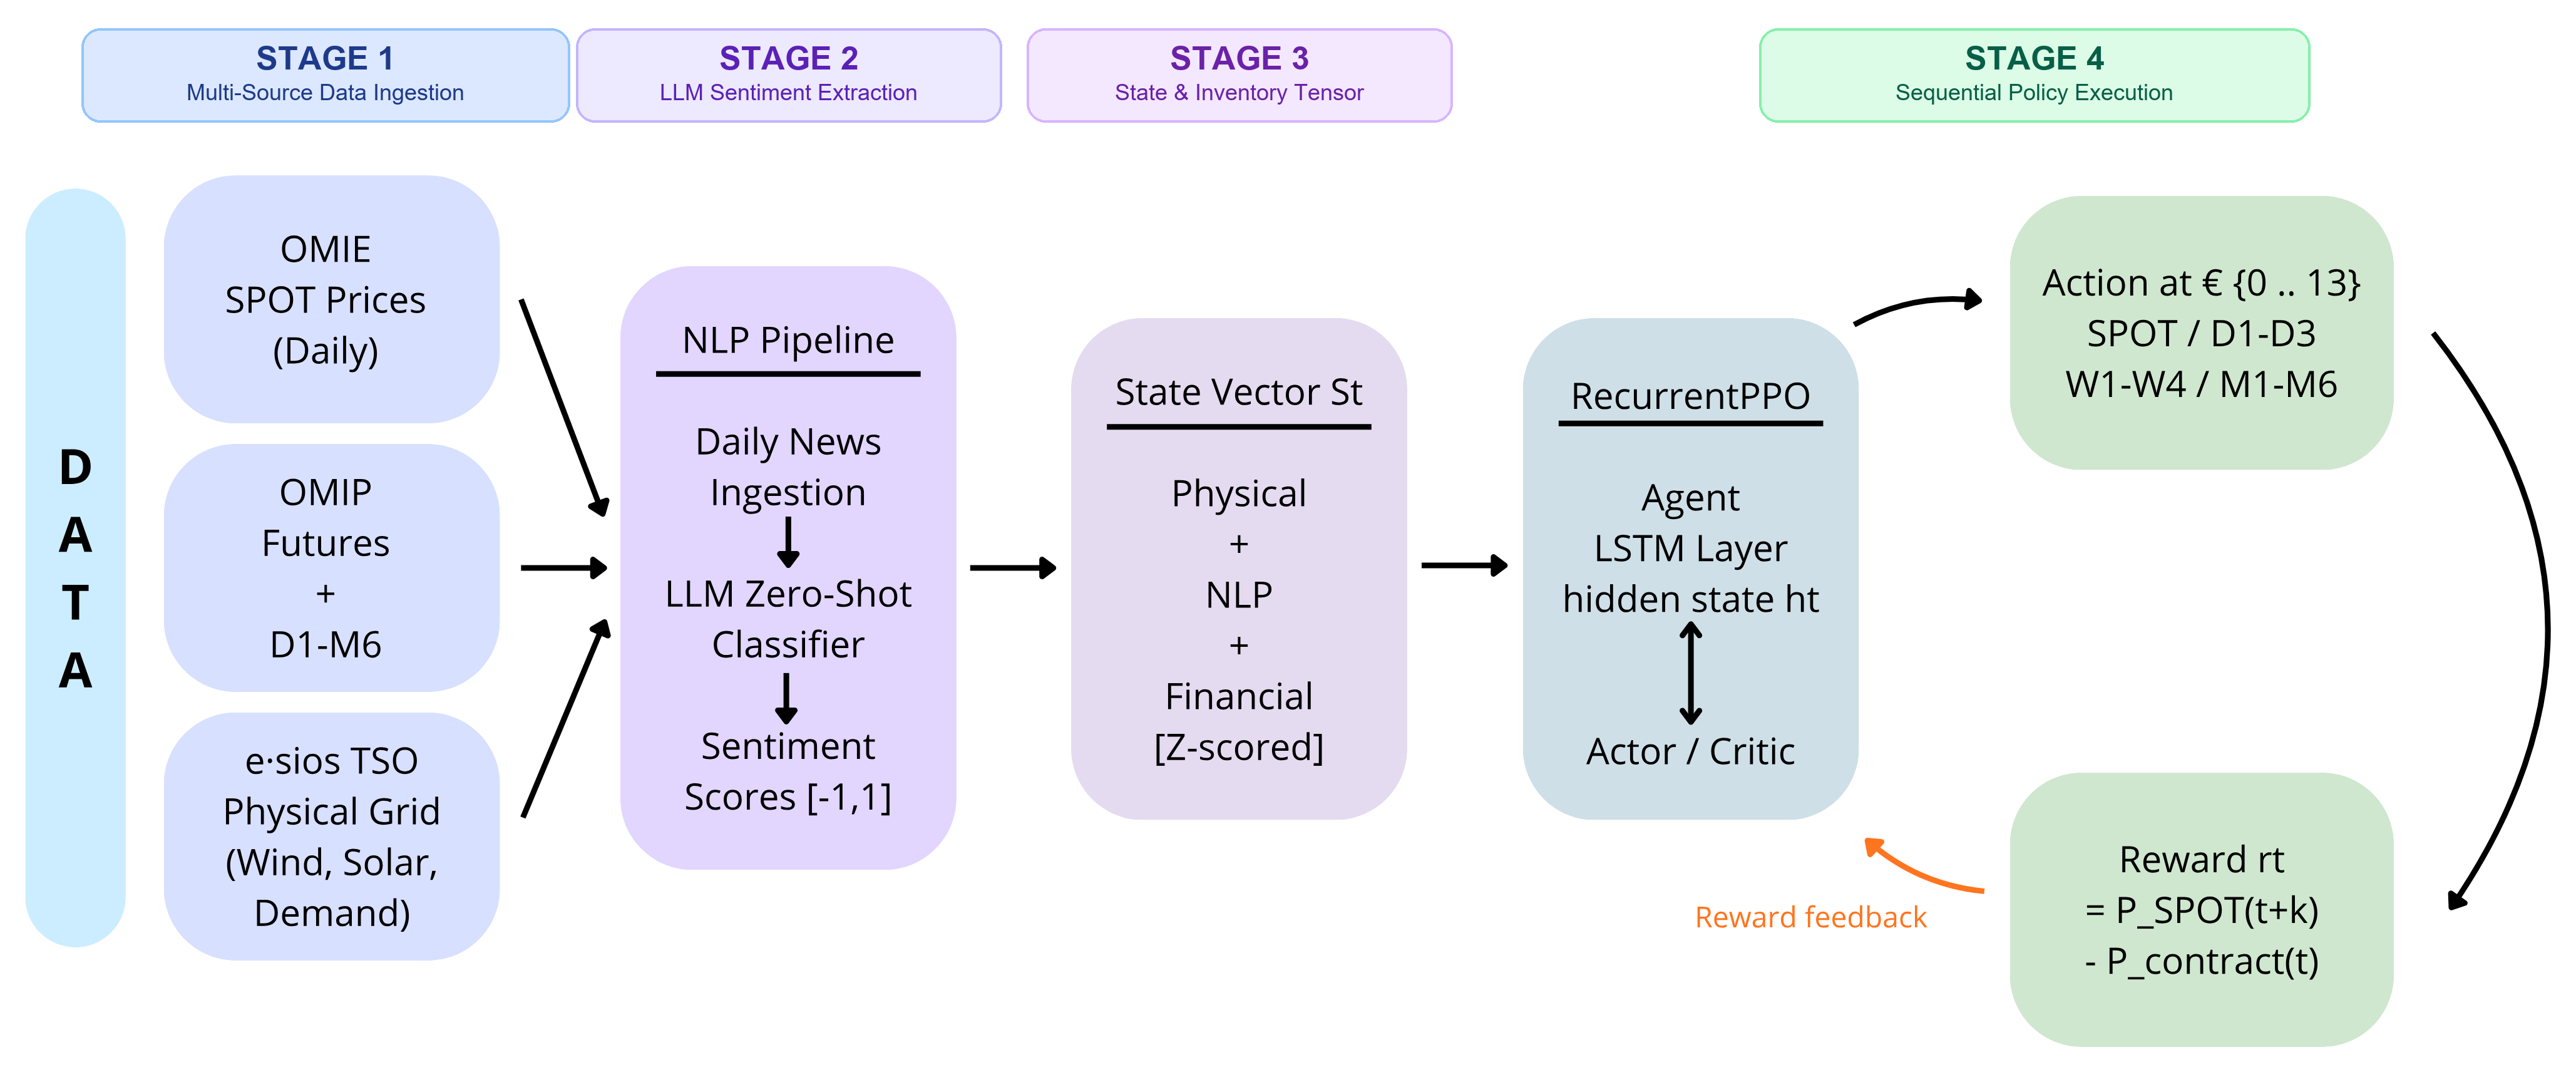
\includegraphics[width=\textwidth]{fig7_system_architecture.png}
    \caption{End-to-end system architecture and operational pipeline of the hybrid DRL and LLM procurement framework across four sequential operational stages.}
    \label{fig:architecture}
\end{figure*}

The methodology developed in this study operates as a continuous, end-to-end pipeline designed to emulate the daily decision-making process of an industrial energy purchasing department. As illustrated in \Cref{fig:architecture}, the logical architecture comprises four sequential operational stages: (1)~\textit{Multi-source data ingestion and synchronization}, where daily physical generation by technology, aggregate electrical demand, and international cross-border transfer capacities from the Transmission System Operator (TSO, Red El\'ectrica de Espa\~na, REE) are merged with daily clearing prices from the market operator (OMIE) and forward settlement curves from the derivatives exchange (OMIP), synchronised strictly at day $t-1$ (23:59~CET); (2)~\textit{Deterministic zero-shot NLP sentiment extraction}, wherein energy and macroeconomic news articles are processed natively using Meta's Llama-3 model under deterministic inference ($T=0.0$, strict JSON schema) to extract 10 domain-specific continuous sentiment scores ($\phi_1, \dots, \phi_{10}$) covering short/medium/long-term outlooks, fuel availability, and regulatory risks; (3)~\textit{Unified state and physical inventory construction}, where the environment constructs a 7-day lookback observation matrix of market features combined with a 400-day forward procurement inventory vector ($\mathbf{c}_t$) with sentinel encoding ($-10.0$ for unhedged delivery slots), tracking forward commitments and delivery coverage; and (4)~\textit{Sequential reinforcement learning execution}, where the deep sequential policy (Recurrent Proximal Policy Optimization, RecurrentPPO, or GTrXL Transformer) observes state vector $\mathbf{o}_t$ and outputs a discrete forward hedging action $a_t \in \{0, \dots, 13\}$, updating physical delivery inventory, executing financial cash flows, and receiving daily unit savings rewards.

\subsection{Data Pipeline and Information Set Timing}
\label{subsec:nlp}

The input space integrates two complementary data streams: a physical/financial market stream and an NLP-derived macroeconomic sentiment stream. To benchmark electricity procurement, the consumption profile is normalised to a continuous unit baseload demand of $E_{\text{load}, d} = 24$~MWh/day per MW of continuous electrical capacity ($1\text{ MW} \times 24\text{ h} = 24\text{ MWh}$). This canonical unit-capacity benchmark represents an industrial consumer schedule whose procurement savings and risk metrics scale linearly to any facility size (e.g., $E_{\text{load}, d} = 4{,}800\text{ MWh/day}$ for a $200$~MW large-scale industrial facility or hyperscale data center \cite{masanet2020recalibrating, iea2024electricity}). Normalizing to unit baseload capacity ensures that the reported results reflect market settlement dynamics without depending on arbitrary enterprise scale, while unit orders of 1~MW represent standard exchange lot sizes that are readily absorbable under normal OMIP order-book liquidity. To evaluate execution robustness, policy sensitivity is tested under hypothetical linear transaction cost levels of 0, 0.10, and 0.25~\texteuro/MWh (Section~\ref{subsec:trans_costs}).

To prevent look-ahead bias and temporal data leakage, the procurement environment is formulated as a daily derivative settlement backtest operating on official clearing and settlement prices from OMIP and OMIClear. The policy selects forward contract commitments using information available through day $t-1$ (23:59~CET); the selected exposure is subsequently valued at the official day-$t$ OMIP closing settlement price $P_{a, t}$. This represents a settlement-valued backtest evaluating settlement-implied procurement efficiency rather than an order-book execution simulation. \Cref{tab:information_set} details the exact source, real-world publication timing, and temporal lag applied to each variable category to ensure causal state construction.

\begin{table*}[!t]
\centering
\footnotesize
\setlength{\tabcolsep}{4pt}
\caption{Information set, sources, publication timing, and temporal lags ensuring causal state construction without look-ahead bias.}
\label{tab:information_set}
\begin{tabularx}{\linewidth}{@{} >{\hsize=1.30\hsize\raggedright\arraybackslash}X
                                  >{\hsize=0.80\hsize\raggedright\arraybackslash}X
                                  >{\hsize=0.95\hsize\raggedright\arraybackslash}X
                                  >{\hsize=0.90\hsize\raggedright\arraybackslash}X
                                  >{\hsize=1.05\hsize\raggedright\arraybackslash}X@{}}
\toprule
\textbf{Variable Category} & \textbf{Data Source} & \textbf{Publication Timing} & \textbf{Decision Step} & \textbf{Applied Lag} \\
\midrule
Physical Generation & TSO (e-sios / REE) & Day $t-1$, 23:59 CET & Day $t$ Trading Step & Lag $t-1$ (Realised) \\
Total Demand \& Interconnection & TSO (e-sios / REE) & Day $t-1$, 23:59 CET & Day $t$ Trading Step & Lag $t-1$ (Realised) \\
Day-Ahead SPOT Price ($P_{\text{SPOT}}$) & OMIE & Day $t-1$, 13:00 CET & Day $t$ Trading Step & Lag $t-1$ (Realised) \\
Forward Derivatives ($P_{a, t-1}$) & OMIP & Day $t-1$, 18:00 CET & Day $t$ Trading Step & Lag $t-1$ (Settlement) \\
Macroeconomic News Sentiment ($\phi$) & Google News / RSS & Day $t-1$, 23:59 CET & Day $t$ Trading Step & Retrospective composite ($t-1$) \\
\bottomrule
\end{tabularx}
\end{table*}

The textual data stream aggregates news from specialized energy and economic media (e.g., \textit{ember-energy.org}, \textit{elEconomista}, \textit{Europa Press}). As illustrated in \Cref{fig:llm_pipeline}, the extraction pipeline processes daily Spanish and international news feeds through a local Ollama instance running Llama-3 8B-Instruct with strict JSON schemas.

\begin{figure*}[!t]
    \centering
    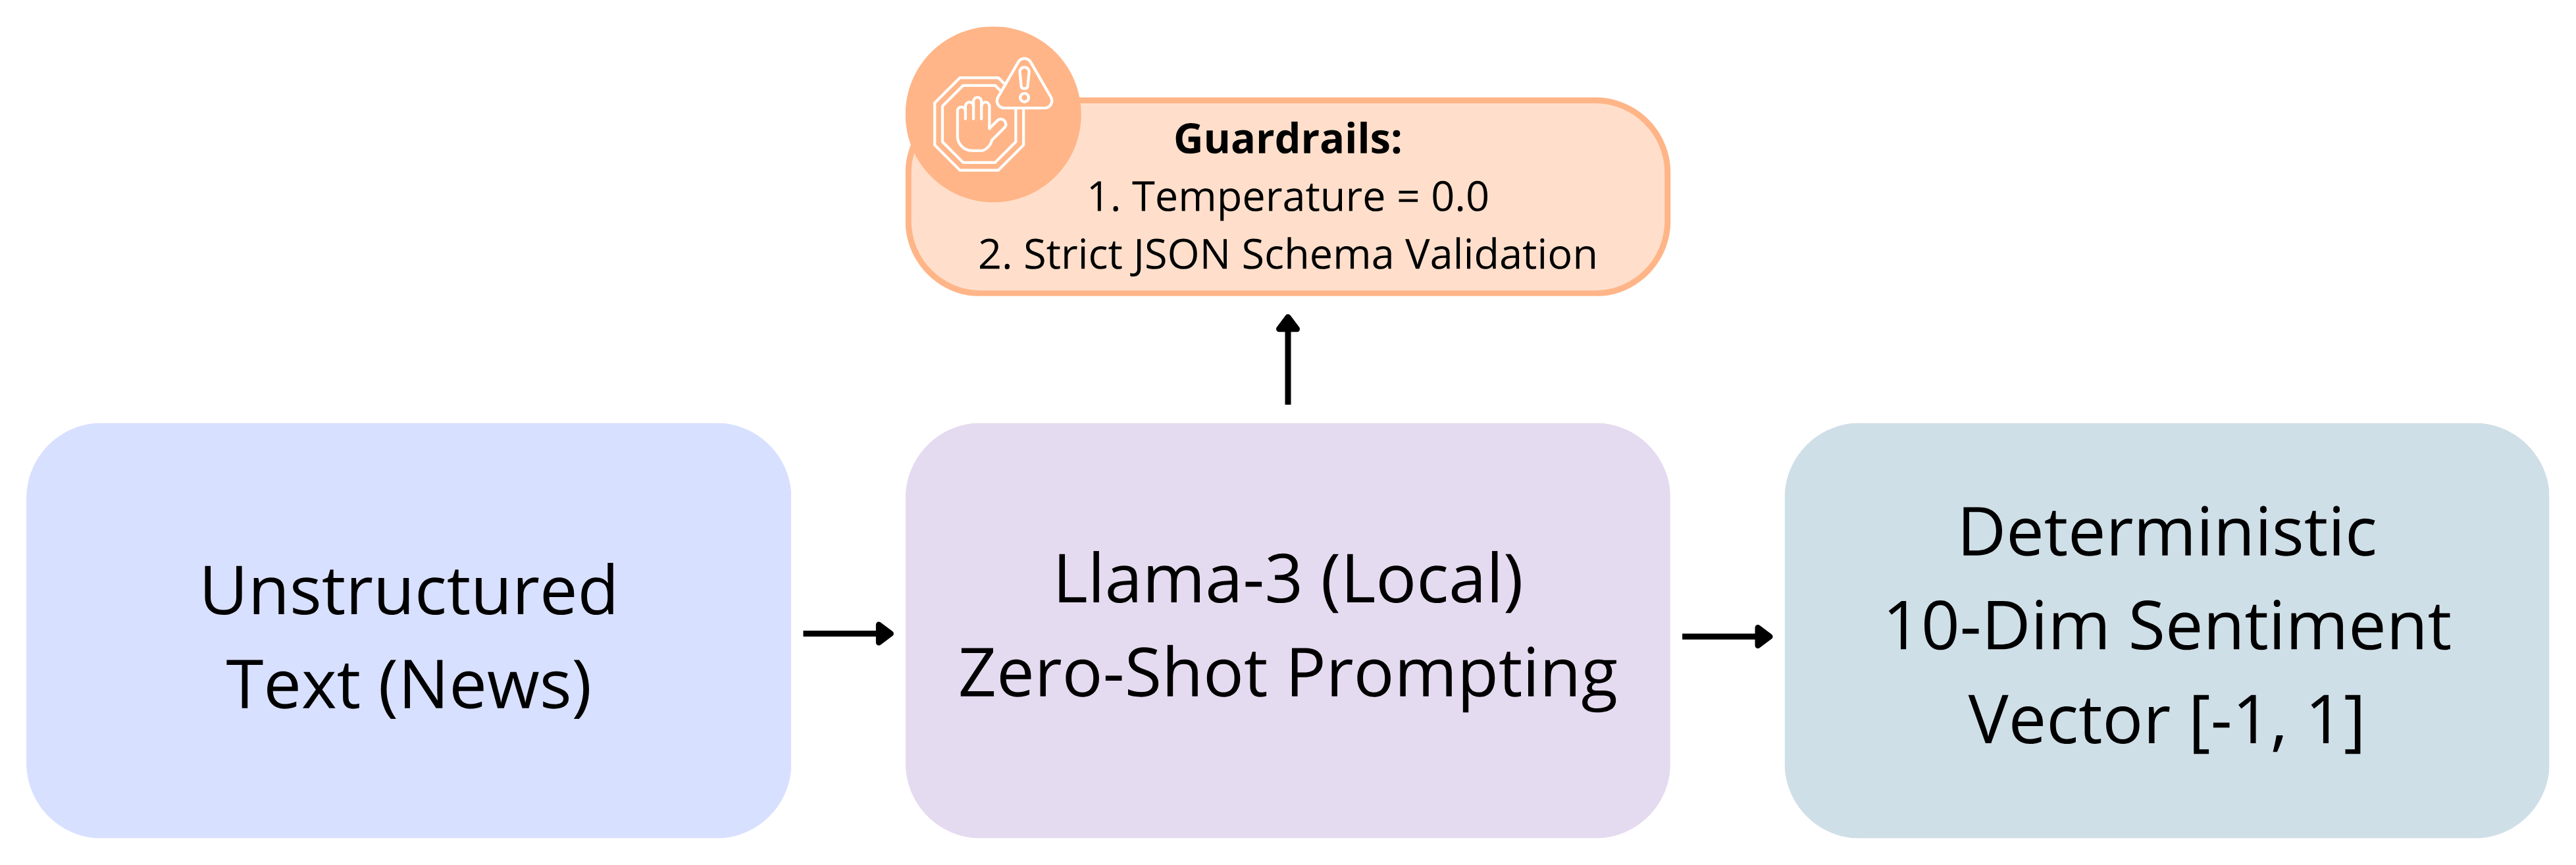
\includegraphics[width=0.70\textwidth]{fig8_llm_pipeline.png}
    \caption{LLM sentiment extraction pipeline with operational guardrails ($T=0.0$ and JSON Schema validation) converting unstructured news into the policy state vector.}
    \label{fig:llm_pipeline}
\end{figure*}

To eliminate consumer-oriented noise, a preliminary zero-shot classification is performed using the Llama-3 model. The filtering prompt instructs the LLM to act as an energy market analyst and strictly discard consumer-oriented news (e.g., residential tariffs), keeping only structural, macroeconomic, or geopolitical news.
The approved articles are then processed by a local Ollama server running the \textit{Llama-3 8B-Instruct} model (using Q4\_K\_M 4-bit quantisation) for sentiment scoring. To obtain reproducible, machine-readable structured outputs suitable for integration into a continuous DRL pipeline, deterministic decoding under the reported model and software configuration is enforced ($T=0.0$, top-$p = 1.0$, and a strict JSON schema). Using a zero-shot prompt design~\cite{yin2019benchmarking} and a context window of 8,192 tokens, the LLM maps the unstructured text into ten continuous sentiment scores, each normalised to the interval $[-1,+1]$:
$\phi_1$~(short-term market outlook),
$\phi_2$~(medium-term outlook),
$\phi_3$~(long-term outlook),
$\phi_4$~(LLM confidence score),
$\phi_5$~(LNG gas sentiment),
$\phi_6$~(CO\textsubscript{2} ETS sentiment),
$\phi_7$~(MIBEL regulatory impact),
$\phi_8$~(climate and generation mix),
$\phi_9$~(geopolitical risk index), and
$\phi_{10}$~(macroeconomic demand).

Scores are aggregated on a strictly daily, retrospective basis: for any trading day $t$, only news published strictly up to day $t-1$ are processed, using a timestamping scheme designed to avoid look-ahead from the available information set. Numerical features are subsequently normalised via Z-score standardisation computed strictly over the training set.

\subsection{Mathematical Formulation of the Procurement MDP}
\label{subsec:mdp}

We formulate the sequential multi-horizon energy procurement problem through a finite-memory Markov Decision Process (MDP) approximation of an underlying partially observable market process (POMDP)~\cite{puterman1994mdp} defined by the tuple $(\mathcal{S}, \mathcal{A}, \mathcal{O}, \mathcal{P}, \mathcal{R}, \gamma)$. In this formulation, latent macroeconomic, regulatory, and weather dynamics are partially observed through historical lookback windows and zero-shot NLP sentiment indices, mapping underlying environmental states $s_t \in \mathcal{S}$ to compact agent observations $\mathbf{o}_t \in \mathcal{O}$.

To distinguish between environmental information and the inputs supplied to the policy, at each trading day $t$ the underlying environment state $s_t \in \mathcal{S}$ is defined by the historical market matrix, the locked unit price vector, and the binary delivery coverage mask:
\begin{equation}
\begin{aligned}
    s_t = \Big( &\mathbf{X}_t \in \mathbb{R}^{7 \times d_{\text{feat}}},\; \mathbf{c}_t \in \mathbb{R}^{H}, \\
    &\mathbf{m}_t \in \{0, 1\}^{H} \Big)
\end{aligned}
\label{eq:state_space}
\end{equation}
where $\mathbf{X}_t \in \mathbb{R}^{7 \times d_{\text{feat}}}$ represents the 7-day lookback window of all normalised market fundamentals, forward settlement curves, and NLP sentiment variables ($d_{\text{feat}}$ dimensions). The vector $\mathbf{c}_t = [c_t(1), c_t(2), \dots, c_t(H)]^{\top} \in \mathbb{R}^{H}$ records the unnormalized unit procurement prices locked for future delivery dates $t+\delta$ ($\delta \in \{1, \dots, H\}$) over a maximum horizon of $H = 400$~days, while $\mathbf{m}_t \in \{0, 1\}^H$ tracks binary delivery coverage.

To provide a compact representation to the neural policy networks without redundant binary masks, the agent receives the observation vector $\mathbf{o}_t \in \mathbb{R}^{7 d_{\text{feat}} + 400}$:
\begin{equation}
    \mathbf{o}_t = \big[ \text{vec}(\mathbf{X}_t);\, \tilde{\mathbf{c}}_t \big] \in \mathbb{R}^{(7 \times d_{\text{feat}}) + 400}
    \label{eq:observation_vector}
\end{equation}
For \texttt{Dataset\_\allowbreak M8\_\allowbreak Physical\_\allowbreak NLP} ($d_{\text{feat}} = 45$), this yields a 715-dimensional observation vector $\mathbf{o}_t \in \mathbb{R}^{715}$. The vector $\tilde{\mathbf{c}}_t \in \mathbb{R}^H$ is the standardized inventory vector with sentinel encoding:
\begin{equation}
    \tilde{c}_t(\delta) = 
    \begin{cases}
        z\big(c_t(\delta)\big), & \text{if } m_t(\delta) = 1 \\
        -10.0, & \text{if } m_t(\delta) = 0
    \end{cases}
    \label{eq:sentinel_encoding}
\end{equation}
Here, $z(\cdot)$ denotes standard $z$-score normalization based on training distribution statistics (where normalized prices predominantly lie in $[-3.0, +3.0]$). The value $-10.0$ serves strictly as a non-economic sentinel encoding outside the empirical standardized range $[-3.0, +3.0]$, allowing the neural networks to unambiguously differentiate uncommitted forward delivery slots from committed positions without introducing an extra binary mask dimension in the observation space.

The action space $\mathcal{A} = \{a_0, a_1, \dots, a_{13}\}$ comprises 14 discrete actions representing standardized constant-maturity rolling forward products calibrated to daily OMIP closing settlement curves. Rather than trading exchange-listed calendar instruments directly, we construct synthetic constant-maturity products mapped to fixed forward offsets:
\begin{itemize}
    \item $a_0$: Open SPOT procurement (unhedged, physical power purchased at the daily SPOT clearing price).
    \item $a_1, a_2, a_3$: Daily forward contracts ($D_1, D_2, D_3$), with relative delivery offsets $\Delta(a_1) = \{1\}$, $\Delta(a_2) = \{2\}$, and $\Delta(a_3) = \{3\}$.
    \item $a_4, \dots, a_7$: Weekly forward contracts ($W_1, \dots, W_4$), covering calendar weeks $[\delta_{\text{mon}} + 7(k-4),\, \delta_{\text{mon}} + 7(k-4) + 6]$ for $k \in \{4, 5, 6, 7\}$, with $\delta_{\text{mon}}$ days to next Monday.
    \item $a_8, \dots, a_{13}$: Monthly forward contracts ($M_1, \dots, M_6$), covering target month $m = \text{month}(t) + (k-7)$ over delivery offset range $\Delta(a_k)$.
\end{itemize}
Weekend and market holiday delivery slots inherit the forward delivery commitments locked during previous active trading sessions; unhedged weekend slots settle at the official OMIE weekend SPOT clearing price. Because OMIE physical spot clearing operates 365 days a year while OMIP derivative trading operates exclusively on official exchange business days ($\approx 252$ days/year, closing on weekends and TARGET2/OMIP bank holidays), non-trading days are handled via a deterministic \texttt{NO\_TRADE} default: no new forward commitments can be initiated, and power delivery is procured at SPOT unless previously covered by a maturing forward contract locked on a prior trading session. When a forward contract has no active quotation on an exchange session, or when selecting it would violate non-overlapping baseload delivery constraints ($\sum_{\delta \in \Delta(a)} m_t(\delta) > 0$), the action is flagged as invalid and incurs the penalty $\lambda_{\text{pen}}$, preserving strict operational validity across all contract horizons ($D_1$--$M_6$).

Each forward contract $a \in \mathcal{A} \setminus \{a_0\}$ selected at trading day $t$ is valued at the official OMIP daily closing settlement price $P_{a, t}$ for that day, whereas input state features condition exclusively on information available up to day $t-1$ (23:59~CET). The position sizing maps each action to a continuous 100\% base-load volume hedge ($E_{\text{load}, d} = 24$~MWh/day per MW of continuous baseload capacity).

The environmental state transitions and forward hedging commitments unfold sequentially. Upon selecting action $a_t$ at day $t$, action validity is verified against existing inventory: the action is valid if no covered day overlaps ($\sum_{\delta \in \Delta(a_t)} m_t(\delta) = 0$) and the quoted price $P_{a_t, t}$ is valid. If valid, the intermediate post-action inventory vector $\mathbf{c}_t^+$ and mask $\mathbf{m}_t^+$ are updated:
\begin{equation}
\begin{aligned}
    c_t^+(\delta) &= 
    \begin{cases}
        P_{a_t, t}, & \text{if } \delta \in \Delta(a_t) \\
        c_t(\delta), & \text{otherwise}
    \end{cases}, \\
    m_t^+(\delta) &= 
    \begin{cases}
        1, & \text{if } \delta \in \Delta(a_t) \\
        m_t(\delta), & \text{otherwise}
    \end{cases}
    \qquad \forall\,\delta \in \{1, \dots, H\}
\end{aligned}
\label{eq:inventory_update}
\end{equation}
If invalid, the position vector remains unchanged ($\mathbf{c}_t^+ = \mathbf{c}_t$, $\mathbf{m}_t^+ = \mathbf{m}_t$) and an invalid penalty indicator $\mathbb{I}_{\text{invalid}}(a_t) = 1$ is triggered. Using an internal penalty in the reward function rather than hard action masking maintains continuous, unconstrained policy gradient estimation across the full 14-dimensional action space during PPO optimization, allowing the policy to smoothly learn feasible operational boundaries.

When advancing from day $t$ to day $t+1$:
\begin{enumerate}
    \item \textbf{Settlement of Delivery Day $t+1$:} The position $c_t^+(1)$ (with mask $m_t^+(1)$) matures. The effective unit procurement cost $P_{\text{eff}, t+1}$ realised for delivery day $t+1$ is:
    \begin{equation}
        P_{\text{eff}, t+1} = m_t^+(1) \cdot c_t^+(1) + \big(1 - m_t^+(1)\big) \cdot P_{\text{SPOT}, t+1}
        \label{eq:effective_cost}
    \end{equation}
    \item \textbf{Inventory Shift Transition:} The remaining forward commitments shift by one calendar day into state $s_{t+1}$:
    \begin{equation}
    \begin{aligned}
        c_{t+1}(\delta) &= c_t^+(\delta + 1), \\
        m_{t+1}(\delta) &= m_t^+(\delta + 1), \quad \forall\,\delta \in \{1, \dots, H-1\}
    \end{aligned}
    \label{eq:inventory_shift}
    \end{equation}
    with boundary condition $c_{t+1}(H) = -10.0, m_{t+1}(H) = 0$.
\end{enumerate}

Table~\ref{tab:action_settlement_mapping} summarizes the execution and settlement mapping across contract types, confirming consistent temporal indexing. For weekly contracts $W_k$ ($k \in \{1, 2, 3, 4\}$), let $\text{wd}(t) \in \{0, \dots, 6\}$ denote the weekday of trading session $t$ ($0 = \text{Monday}$). The delivery window covers the target Monday-to-Sunday calendar week:
\begin{align}
    \delta_{\text{start}}(W_k, t) &= d_{\text{next\_Mon}}(t) + 7(k-1) \\
    \delta_{\text{end}}(W_k, t) &= \delta_{\text{start}}(W_k, t) + 6
\end{align}
where $d_{\text{next\_Mon}}(t) = 7 - \text{wd}(t)$ (or 7 if $\text{wd}(t)=0$). For monthly contracts $M_k$ ($k \in \{1, \dots, 6\}$), the delivery window spans the full calendar month starting on the 1st of month $m_t + k$ and ending on its last day. 

To prevent terminal truncation bias near dataset boundaries, the environment verifies that each contract's delivery window falls strictly within the historical series and inventory bounds ($0 \le \delta_{\text{start}}$ and $t + \delta_{\text{end}} \le T_{\text{dataset}}, \delta_{\text{end}} < H$). Any action whose delivery extends beyond available market records is masked as an invalid decision ($\lambda_{\text{pen}} = 1.0$~\texteuro/MWh penalty) and defaults to SPOT clearing.

\begin{table*}[!t]
\centering
\footnotesize
\setlength{\tabcolsep}{4pt}
\caption{Action execution, delivery window offsets, state entry, and settlement timing mapping.}
\label{tab:action_settlement_mapping}
\begin{tabularx}{\linewidth}{@{} >{\hsize=0.65\hsize\raggedright\arraybackslash}X
                                  >{\hsize=1.15\hsize\raggedright\arraybackslash}X
                                  >{\hsize=1.20\hsize\raggedright\arraybackslash}X
                                  >{\hsize=0.95\hsize\raggedright\arraybackslash}X
                                  >{\hsize=1.05\hsize\raggedright\arraybackslash}X@{}}
\toprule
\textbf{Action ($a_t$)} & \textbf{Delivery Window ($\tau$)} & \textbf{Delivery Offsets $[\delta_s, \delta_e]$} & \textbf{Settlement Day} & \textbf{Effective Cost Realised} \\
\midrule
SPOT ($a_0$) & $t+1$ & Unhedged ($m_t^+(1) = 0$) & $t+1$ & $P_{\text{eff}, t+1} = P_{\text{SPOT}, t+1}$ \\
$D_1$ ($a_1$) & $t+1$ & $[1, 1]$ & $t+1$ & $P_{\text{eff}, t+1} = P_{D_1, t}$ \\
$D_2$ ($a_2$) & $t+2$ & $[2, 2]$ & $t+2$ & $P_{\text{eff}, t+2} = P_{D_2, t}$ \\
$D_3$ ($a_3$) & $t+3$ & $[3, 3]$ & $t+3$ & $P_{\text{eff}, t+3} = P_{D_3, t}$ \\
$W_k$ ($a_4$--$a_7$) & Next $k$-th Mon--Sun week & $[d_{\text{Mon}}+7(k-1),\, d_{\text{Mon}}+7k-1]$ & $\tau \in [t+\delta_s, t+\delta_e]$ & $P_{\text{eff}, \tau} = P_{W_k, t}$ \\
$M_k$ ($a_8$--$a_{13}$) & Target calendar month $(m_t+k)$ & $[d_{\text{1st}},\, d_{\text{last}}]$ & $\tau \in [t+\delta_s, t+\delta_e]$ & $P_{\text{eff}, \tau} = P_{M_k, t}$ \\
\bottomrule
\end{tabularx}
\end{table*}

In European wholesale power markets, derivatives listed on OMIP (such as SPEL Baseload Futures) are financially-settled derivative contracts cleared through OMIClear. In accordance with the OMIClear Clearing Rulebook~\cite{omiclear2023rulebook}, the cash flows of a buy forward position entered on trading day $t$ at quote $F_{t, \text{prod}} = P_{a_t, t}$ covering delivery period $\mathcal{D}_{\text{prod}}$ (with total contract volume $Q_{\text{prod}} = q \cdot |\mathcal{D}_{\text{prod}}|$, where $q = 24$~MWh/day represents the daily baseload volume per MW of continuous capacity) are resolved in two formal stages:
\begin{enumerate}
    \item \textbf{Trading Stage (up to Last Trading Day, $\text{LTD}$):} Daily mark-to-market variation margins accumulate across the total contract volume from entry day $t$ to the contract's last trading day $\text{LTD}$:
    \begin{equation}
    \begin{aligned}
        \text{CF}_{\text{total}} &= \sum_{k=t+1}^{\text{LTD}} \big( F_{k, \text{prod}} - F_{k-1, \text{prod}} \big) \cdot Q_{\text{prod}} \\
        &= \big( F_{\text{LTD}, \text{prod}} - F_{t, \text{prod}} \big) \cdot Q_{\text{prod}}
    \end{aligned}
    \label{eq:cfd_trading_stage}
    \end{equation}
    where $F_{\text{LTD}, \text{prod}}$ is the final closing settlement price on the last trading session prior to physical delivery. Amortising this gain evenly across the $|\mathcal{D}_{\text{prod}}|$ delivery days yields a daily margin cash flow $\text{CF}_{\text{margin}, d}$:
    \begin{equation}
    \begin{aligned}
        \text{CF}_{\text{margin}, d} &= \frac{1}{|\mathcal{D}_{\text{prod}}|} \big( F_{\text{LTD}, \text{prod}} - F_{t, \text{prod}} \big) \cdot Q_{\text{prod}} \\
        &= \big( F_{\text{LTD}, \text{prod}} - F_{t, \text{prod}} \big) \cdot q
    \end{aligned}
    \label{eq:cfd_daily_margin}
    \end{equation}
    \item \textbf{Delivery Stage (Delivery Settlement Value, $\text{DSV}$):} During each delivery day $d \in \mathcal{D}_{\text{prod}}$, OMIClear calculates the daily financial Delivery Settlement Value for volume $q$ based on the difference between the daily OMIE Spot Reference Price $P_{\text{SPOT}, d}$ and the final futures settlement price $F_{\text{LTD}, \text{prod}}$:
    \begin{equation}
        \text{DSV}_d = \big( P_{\text{SPOT}, d} - F_{\text{LTD}, \text{prod}} \big) \cdot q
        \label{eq:cfd_delivery_stage}
    \end{equation}
    \item \textbf{Physical Spot Procurement in OMIE:} The consumer procures its required continuous baseload energy $q = 24$~MWh in the physical day-ahead market (OMIE) at spot clearing cost $-P_{\text{SPOT}, d} \cdot q$.
\end{enumerate}
Summing the amortised trading-stage variation margin $\text{CF}_{\text{margin}, d}$, the daily delivery settlement value $\text{DSV}_d$, and the physical OMIE spot payment yields the total net procurement cash outflow $\text{CF}_{\text{net}, d}$ for each delivery day $d \in \mathcal{D}_{\text{prod}}$:
\begin{equation}
\begin{aligned}
    \text{CF}_{\text{net}, d} &= - P_{\text{SPOT}, d} \cdot q + \text{DSV}_d + \text{CF}_{\text{margin}, d} \\
    &= - P_{\text{SPOT}, d} \cdot q + \big( P_{\text{SPOT}, d} - F_{\text{LTD}, \text{prod}} \big) \cdot q \\
    &\quad + \big( F_{\text{LTD}, \text{prod}} - F_{t, \text{prod}} \big) \cdot q \\
    &= - F_{t, \text{prod}} \cdot q = - P_{a_t, t} \cdot q
\end{aligned}
\label{eq:net_cashflow}
\end{equation}
Dividing by daily baseload volume $q$ yields the effective unit supply cost $P_{\text{eff}, d} = F_{t, \text{prod}} = P_{a_t, t}$, which is scale-invariant. Under standard frictionless market assumptions (zero execution fees, zero bid-ask half-spreads, and frictionless collateral financing), financial derivative hedging is algebraically identical to locking the unit supply cost at the forward quote $P_{a_t, t}$.

The MDP reward function $\mathcal{R}$ guides sequential policy optimization by measuring unit savings on the immediate settlement day relative to the unhedged SPOT benchmark:
\begin{equation}
    r_t = \big( P_{\text{SPOT}, t+1} - P_{\text{eff}, t+1} \big) - R_{\text{penalty}} \cdot \mathbb{I}_{\text{invalid}}(a_t)
    \label{eq:reward_formal}
\end{equation}
where $R_{\text{penalty}} = 20.0$~\texteuro/MWh is an internal MDP optimization penalty applied during policy training whenever the agent selects an invalid action (e.g., attempting to purchase a contract on an unavailable trading day, or selecting an action whose forward delivery window overlaps already committed inventory in $\mathbf{m}_t$). When an invalid action occurs, the order is rejected without state update, the consumer default clears that day's physical demand at the actual day-ahead spot price ($P_{\text{eff}, t+1} = P_{\text{SPOT}, t+1}$), and the reported out-of-sample economic cost accounts strictly for the physical market expenditure ($g_t = 0$), ensuring that training penalties do not distort empirical procurement metrics. An explicit terminal salvage penalty $\lambda_{\text{term}} = 1.0$~\texteuro/MWh is defined for unliquidated positions at the final horizon boundary. The discount factor is set to $\gamma = 0.99$.

Let $g_t = P_{\text{SPOT}, t} - P_{\text{eff}, t}$ denote the daily unit savings (\texteuro/MWh) realised on calendar delivery day $t \in \{1, \dots, T\}$, and let $G_t = \sum_{i=1}^t g_i$ denote the cumulative savings path up to day $t$ (with $G_0 = 0$). Performance and financial risk are evaluated across five formal metrics: Percentage Savings ($S_{\%}$), Cumulative Unit Differential ($S_{\text{cum}}$), Downside Semi-deviation ($\sigma_-$), Conditional Value at Risk ($\text{CVaR}_{0.95}$), and Maximum Drawdown ($\text{Max DD}$):
\begin{align}
    S_{\%} &= \frac{\sum_{t=1}^T g_t}{\sum_{t=1}^T P_{\text{SPOT}, t}} \times 100\% = \frac{\sum_{t=1}^T (P_{\text{SPOT}, t} - P_{\text{eff}, t})}{\sum_{t=1}^T P_{\text{SPOT}, t}} \times 100\% \label{eq:metric_savings_pct} \\
    S_{\text{cum}} &= \sum_{t=1}^T g_t \quad [\text{\texteuro/MWh}] \label{eq:metric_savings_cum} \\
    \sigma_- &= \sqrt{\frac{1}{T} \sum_{t=1}^T \big(\min(g_t, 0)\big)^2} \quad [\text{\texteuro/MWh}] \label{eq:metric_semidev} \\
    \text{CVaR}_{0.95} &= \frac{1}{\lfloor 0.05 \cdot T \rfloor} \sum_{k=1}^{\lfloor 0.05 \cdot T \rfloor} g_{(k)} \quad [\text{\texteuro/MWh}] \label{eq:metric_cvar} \\
    \text{Max DD} &= \max_{1 \le t \le T} \left( \max_{1 \le u \le t} G_u - G_t \right) \quad [\text{\texteuro/MWh}] \label{eq:metric_maxdd}
\end{align}
where $g_{(1)} \le g_{(2)} \le \dots \le g_{(T)}$ represent the ascending order statistics of daily unit savings $g_t$. For multi-year Walk-Forward evaluations across the 40 test blocks ($T = D_{\text{eval}} = 374$ evaluated days), aggregate percentage savings represent an expenditure-weighted average across annual sub-horizons: $S_{\%, \text{agg}} = \sum_y w_y S_{\%, y}$, where weights $w_y = \sum_{t \in y} P_{\text{SPOT}, t} / \sum_{t=1}^T P_{\text{SPOT}, t}$ reflect time-varying wholesale spot prices ($w_{2023} \approx 37.6\%$, $w_{2024} \approx 29.3\%$, $w_{2025} \approx 26.6\%$, and $w_{2026} \approx 6.5\%$), yielding $+6.04\%$ multi-year savings ($\sum g_t / \sum P_{\text{SPOT}} = 1{,}486.39 / 24{,}595.50$), with average daily unit savings of $3.97$~\texteuro/MWh over the 374 evaluated days (where mean evaluated spot price was $65.76$~\texteuro/MWh; $3.974 / 65.763 = 6.04\%$), distinct from the broader 1,242-day multi-year spot average of $55.40$~\texteuro/MWh. Under this convention, $\text{CVaR}_{0.95}$ measures the lower-tail Expected Shortfall at 5\% on savings (where negative values represent expected unit deficits in the worst 5\% tail), and $\text{Max DD}$ quantifies the peak-to-trough decline of the cumulative savings trajectory ($0.00$~\texteuro/MWh for Pure SPOT as $g_t \equiv 0$). Total monetary savings scale as $S_{\text{cum}} \times q$~\texteuro/MW.

To evaluate sequential decision-making under partial observability, we compare two distinct policy architectures operating on observation vectors $\mathbf{o}_t$:
\begin{enumerate}
    \item \textbf{RecurrentPPO (LSTM):} Single-layer LSTM ($d_h = 256$ in baseline; $d_h = 64$ in Phase 4 tuned) \cite{hochreiter1997lstm, pleines2022recurrentppo} with hidden state update $h_t = \mathrm{LSTM}(\mathbf{o}_t, h_{t-1}; \theta_{\text{LSTM}})$, feeding separate linear Actor and Critic heads.
    \item \textbf{GTrXL Transformer Comparator:} Gated Transformer-XL architecture \cite{parisotto2020gtrxl, vaswani2017attention} comprising $L = 2$ transformer layers, $H = 4$ attention heads, model dimension $d_{\text{model}} = 64$, memory length $M = 14$, GRU-style gating on skip connections, and layer normalisation.
\end{enumerate}
Both architectures are optimized using Proximal Policy Optimization (PPO) \cite{schulman2017ppo} with Generalized Advantage Estimation (GAE, $\lambda = 0.95$, $\gamma = 0.99$):
\begin{equation}
\begin{aligned}
    \mathcal{L}_{\text{PPO}}(\theta) &= -\hat{\mathbb{E}}_t \left[ \min\left( \rho_t(\theta) \hat{A}_t,\; \mathrm{clip}(\rho_t(\theta), 1-\epsilon, 1+\epsilon) \hat{A}_t \right) \right] \\
    &\quad + c_v L_t^V(\theta) - c_{\text{ent}} \mathcal{H}(\pi_\theta(\cdot \mid \mathbf{o}_t, h_{t-1}))
\end{aligned}
\label{eq:ppo_loss}
\end{equation}
where $\rho_t(\theta) = \frac{\pi_\theta(a_t \mid \mathbf{o}_t, h_{t-1})}{\pi_{\theta_{\text{old}}}(a_t \mid \mathbf{o}_t, h_{t-1})}$, clipping range $\epsilon = 0.2$, value loss coefficient $c_v = 0.5$, and entropy coefficient $c_{\text{ent}} = 0.01$ ($0.0239$ in Phase 4). Optimization is performed using Adam ($\beta_1 = 0.9, \beta_2 = 0.999, \epsilon_{\text{Adam}} = 10^{-8}$) with gradient norm clipping at $0.5$, rollout buffer size $n_{\text{steps}} = 128$ ($64$ in Phase 4), mini-batch size $64$ ($16$ in Phase 4), and 10 optimization epochs per update.

\subsection{Empirical Baseline Analysis: Forward Price Differentials}
\label{subsec:d2_anomaly}

Prior to evaluating the DRL policy, we conduct an empirical baseline analysis by systematically purchasing individual forward contracts across the historical timeline. This test highlights the existence of historical price differentials. We document a persistent D2--SPOT price differential in the evaluated sample: the D2 contract (delivery at $t+2$) exhibited an aggregate forward--spot discount relative to the eventual SPOT price. This empirical discount is consistent with horizon-dependent forward risk premia documented in European electricity derivative markets \cite{huisman2012electricity, woo2001cross, huisman2009electricity}, where forward quotations reflect market-specific hedging incentives and asymmetric risk preferences across clearing horizons. While theoretical literature suggests that short-term forward discounts can arise from hedging pressures under short-term generation uncertainty \cite{schwenen2024renewable}, attributing this differential to specific market agents would require order-book and participant-level bid data; here, we treat it strictly as an empirical benchmark property of the evaluated historical market series. 

\begin{table*}[!t]
\centering
\footnotesize
\setlength{\tabcolsep}{2.5pt}
\caption{Passive procurement performance across the evaluated forward-contract horizons (2023--2026), with annual breakdown for the dominant $D_2$ forward baseline.}
\label{tab:systematic_baselines}
\begin{tabularx}{\linewidth}{@{} >{\raggedright\arraybackslash}X >{\centering\arraybackslash}p{1.6cm} rrrrr@{}}
\toprule
\textbf{Contract / Horizon} & \textbf{Eval.\ Days} & \textbf{Win} & \textbf{Mean PnL} & \textbf{Total PnL} & \textbf{Max DD} & \textbf{Savings} \\
 & & \textbf{Rate} & \textbf{(\texteuro/MWh)} & \textbf{(\texteuro/MWh)} & \textbf{(\texteuro/MWh)} & \textbf{(\%)} \\
\midrule
\multicolumn{7}{l}{\textit{Panel A: Multi-Year Forward Contract Comparison (2023--2026)}} \\
D1 & 1,242 & 50.40\% & 1.65 & 2,044 & 316.18 & 2.37\% \\
\textbf{D2 (Multi-Year)} & \textbf{1,218} & \textbf{59.93\%} & \textbf{8.30} & \textbf{10,104} & \textbf{394.18} & \textbf{11.95\%} \\
D3 & 1,198 & 55.59\% & 4.19 & 5,025 & 412.99 & 5.98\% \\
W1 & 1,088 & 46.32\% & $-5.28$ & $-5,740$ & 7,883 & $-7.27\%$ \\
W2 & 1,081 & 51.43\% & 0.32 & 342 & 4,026 & 0.43\% \\
W3 & 1,074 & 49.81\% & $-2.12$ & $-2,272$ & 6,215 & $-2.92\%$ \\
W4 & 1,067 & 45.27\% & $-4.11$ & $-4,386$ & 7,851 & $-5.77\%$ \\
M1 & 1,065 & 48.83\% & $-1.90$ & $-2,021$ & 5,247 & $-2.67\%$ \\
M2 & 1,037 & 41.27\% & $-8.05$ & $-8,345$ & 11,260 & $-11.72\%$ \\
M3 & 1,006 & 42.45\% & $-13.83$ & $-13,914$ & 14,963 & $-20.72\%$ \\
M4 & 976 & 40.78\% & $-20.24$ & $-19,751$ & 19,730 & $-31.61\%$ \\
M5 & 945 & 29.10\% & $-25.48$ & $-24,073$ & 23,983 & $-41.30\%$ \\
M6 & 884 & 27.71\% & $-27.10$ & $-23,958$ & 23,886 & $-44.29\%$ \\
\midrule
\multicolumn{7}{l}{\textit{Panel B: Systematic $D_2$ Forward Baseline Annual Breakdown}} \\
$D_2$ (2023) & 363 & 60.71\% & 8.86 & 3,225 & 284.15 & 10.07\% \\
$D_2$ (2024) & 366 & 62.02\% & 9.02 & 3,301 & 312.40 & 14.13\% \\
$D_2$ (2025) & 365 & 64.11\% & 8.68 & 3,168 & 295.60 & 13.17\% \\
$D_2$ (2026, 148 cal.\ days) & 148 [102] & 56.08\% & 4.94 & 731 & 225.45 & 11.18\% \\
\bottomrule
\end{tabularx}

\bigskip

\caption{Temporal sample accounting across market data sources, operational decision regimes, and experimental evaluation phases (2023--2026).}
\label{tab:sample_accounting}
\setlength{\tabcolsep}{2.5pt}
\begin{tabularx}{\linewidth}{@{} >{\raggedright\arraybackslash}p{2.8cm} >{\centering\arraybackslash}p{2.3cm} ccc >{\raggedright\arraybackslash}X@{}}
\toprule
\textbf{Sample / Scope} & \textbf{Time Horizon} & \textbf{Calendar} & \textbf{Physical} & \textbf{Decision} & \textbf{Operational Specification and Accounting} \\
 & & \textbf{Days} & \textbf{Delivery} & \textbf{Epochs} & \\
\midrule
Full Calendar Timeline & 01/01/23 -- 31/05/26 & 1,247 & 1,247 & --- & Continuous multi-year calendar horizon ($365 + 366 + 365 + 151$ days across 2023, 2024, 2025, and early 2026). \\
Raw OMIE SPOT Clearing & 01/01/23 -- 31/05/26 & 1,247 & 1,247 & 1,247 & Daily marginal pool price clearing across all 1,247 calendar days without operational interruption. \\
OMIP Aligned Evaluation Sample & 03/01/23 -- 30/05/26 & 1,242 & 1,242 & \textbf{1,242} & Retained market delivery sample ($1{,}242$ days) formed by two continuous sampling intervals: $n_1 = 1{,}094$ historical baseline days (03/01/23 -- 31/12/25: 363 in 2023, 366 in 2024, 365 in 2025; excluding 01/01/23 [Sunday] and 02/01/23 [holiday observation]) and $n_2 = 148$ days in 2026 (03/01/26 -- 30/05/26; excluding 01/01/26 [holiday], 02/01/26 [unaligned forward boundary], and 31/05/26 [Sunday boundary]). The inclusive interval 03/01/23--30/05/26 contains exactly 1,242 calendar dates (excluding the 5 boundary dates from the 1,247 raw calendar timeline). Note that naively summing annual calendar counts ($365 + 366 + 365 + 148 = 1{,}244$) includes 01/01/23 and 02/01/23, which are excluded from the evaluated aligned sample. \\
\midrule
Phase 1--2 Validation & 01/01/25 -- 31/12/25 & 365 & 365 & 261 & Static model ablation \& heuristic screening across 365 delivery days: 261 Monday--Friday operational weekday decision epochs (comprising 256 official OMIP trading sessions and 5 weekday TARGET bank holiday closures) and 104 weekend days (totaling 109 non-trading exchange days where default SPOT settlement applies). \\
Phase 3--4 Out-of-Sample & 03/01/26 -- 30/05/26 & 148 & 148 & \textbf{102} (46) & 148 calendar delivery days comprising 102 official OMIP trading sessions (decision epochs where forward contracts can be selected) and 46 non-trading dates (3 weekday TARGET exchange closures [Good Friday, Easter Monday, Labour Day] and 43 weekend days, where passive default SPOT clearing applies). Across non-trading dates, the simulator executes carryover forward settlement or unhedged default SPOT clearing. \\
\midrule
Walk-Forward Evaluation ($W=1$, Monthly Blocks) & 01/02/23 -- 30/05/26 (40 blocks) & 1,215 & 374 & 374 & Exactly 374 evaluated out-of-sample delivery days across the 40 test months (103 in 2023, 114 in 2024, 113 in 2025, and 44 in 2026), evaluating Days 21 to month-end after a 20-day recurrent hidden state warm-up buffer. \\
\bottomrule
\end{tabularx}
\end{table*}

In addition to passive single-contract benchmarks, we formulate an adaptive trend-following benchmark denoted as the \textit{Rolling Adaptive Spread Rule}. On each active trading session $t$, the heuristic evaluates whether the short-dated $D_2$ forward quotation is priced at a favourable spread relative to the trailing $k$-day simple moving average of cleared spot prices $\overline{P}_{\text{SPOT}, t}^{(k)} = \frac{1}{k} \sum_{i=1}^k P_{\text{SPOT}, t-i}$ using an operational lookback window of $k = 14$ days:
\begin{equation}
    a_t = 
    \begin{cases}
        D_2, & \text{if } P_{D_2, t} < \overline{P}_{\text{SPOT}, t}^{(k)} \text{ and } m_t(2) = 0 \\
        \text{SPOT}, & \text{otherwise}
    \end{cases}
    \label{eq:rolling_adaptive_rule}
\end{equation}
If the delivery slot $t+2$ is already hedged ($m_t(2) = 1$) or if the forward quote exceeds trailing spot averages, the heuristic defaults to unhedged spot procurement. This benchmark represents an intuitive trend-following decision heuristic that captures trailing price deflation without requiring neural network training.

A key institutional development during the sample timeline was the market time unit transition of the Iberian day-ahead market (OMIE) on October 1, 2025, from 24 hourly clearing intervals to 96 quarter-hourly Market Time Units (15-minute MTUs) in compliance with European market integration regulations \cite{omie2025mtu, iea2024electricity}. Throughout our multi-year dataset (2023--2026), the daily SPOT price benchmark $P_{\text{SPOT}, t}$ is consistently defined as the official daily arithmetic mean of cleared marginal prices across all settlement intervals of delivery day $t$:
\begin{equation}
    P_{\text{SPOT}, t} = 
    \begin{cases}
        \frac{1}{24} \sum_{h=1}^{24} P_{t, h}, & t < \text{01/10/2025} \\
        \frac{1}{96} \sum_{q=1}^{96} P_{t, q}, & t \ge \text{01/10/2025}
    \end{cases}
    \label{eq:mtu_standardization}
\end{equation}
ensuring complete mathematical and economic continuity across the pre- and post-transition horizons.

\subsection{Training Methodology and Ablation Study Design}
\label{subsec:training}

From a computational standpoint, all experiments, including the continuous Walk-Forward retraining and Bayesian hyperparameter optimisation, were executed on a dedicated Ubuntu server equipped with an Intel Core Ultra 9 285K processor (24 cores), 64 GB of RAM, and an NVIDIA GeForce RTX 5090 (32 GB) GPU. The LLM sentiment extraction was performed locally using Ollama on the same infrastructure to guarantee data privacy, avoid external API version drift, and ensure computational consistency under deterministic settings. The full 5-seed Walk-Forward evaluation across all 4 update windows ($W \in \{1, 3, 6, 12\}$) required approximately 14.5 GPU hours for RecurrentPPO and 22.0 GPU hours for GTrXL. The Bayesian HPO search (50 Optuna trials per architecture) completed in 18.2 hours. For potential operational deployment, daily policy inference would require only a single forward pass through the policy network ($< 4.2$~ms per decision on standard CPU hardware), while computationally intensive training remains restricted to offline execution.

The training and validation of the agent are structured into four sequential phases to ensure complete traceability of data leakage and look-ahead bias:
\begin{itemize}
    \item \textbf{Phases 1 and 2 (Ablation and Heuristics):} Models are trained on 2023--2024 and evaluated on the 2025 horizon. While strictly out-of-sample for weight updates, the 2025 results are used to select the optimal datasets and discard underperforming heuristics. Consequently, 2025 transitions into a \textit{validation set}, carrying selection bias for future phases.
    \item \textbf{Phase 3 (Walk-Forward Baseline):} A continuous rolling window from 2023 to 2026. Because the datasets were selected based on 2025, the 2026 horizon (3 January -- 30 May 2026, comprising 105 weekday decision epochs represented in the simulator [102 official OMIP trading sessions and 3 TARGET bank holiday closures] within 148 calendar delivery days) represents a strictly forward-looking, sequentially out-of-sample evaluation.
    \item \textbf{Phase 4 (Exploratory Architecture and HPO Analysis):} Hyperparameters are optimized using Optuna across the full Walk-Forward evaluation (including 2026) to determine the optimal attainable capacity of each architecture under tuned hyperparameters. Therefore, the final reported results for Phase 4 are explicitly declared as an \textit{exploratory post-selection capacity analysis}, rather than an unbiased out-of-sample test, establishing the comparative performance limits of Recurrence vs Self-Attention under optimal conditions.
\end{itemize}

In Phase~1 (Model and Data Ablation), we construct eight incremental datasets (\textit{Dataset\_Initial} through \textit{Dataset\_M8\_\allowbreak Physical\_NLP}) to isolate the marginal value of NLP and exogenous features. We train two architectural variants, a standard Multi-Layer Perceptron (MLP) and the LSTM-based RecurrentPPO, across all eight datasets. To evaluate the 2025 horizon, each agent is trained exclusively on 2023--2024 data, ensuring a clean one-year forward evaluation without look-ahead bias.

In Phase~2 (Mitigating Degenerate Policies), initial diagnostic evaluations revealed that the LSTM agent tended to suffer from \textit{entropy collapse}, converging to a low-entropy policy focused on the D2 contract due to the penalty associated with long-term inventory overlap and discounting. To test whether broader multi-horizon hedging can be encouraged, three isolated algorithmic adjustments are evaluated on the LSTM model:
\begin{enumerate}
    \item \textit{Entropy increase}: Raising the entropy coefficient ($c_{\text{ent}}$) in the PPO loss function to $0.05$ to increase the entropy regularization term and encourage broader action exploration.
    \item \textit{Diversification bonus}: Modifying the reward function to include a percentage bonus (+5\% for weekly contracts, +10\% for monthly contracts) upon successful execution.
    \item \textit{Soft action replacement}: Instead of applying a large penalty for an invalid overlapping action, the environment gracefully converts the invalid forward purchase into a SPOT purchase and applies a minor symbolic penalty ($-0.5$\texteuro), effectively acting as a soft alternative to action masking.
\end{enumerate}

In Phase~3 (Continuous Walk-Forward Retraining), we evaluate policy adaptation to market shifts on the out-of-sample test horizon (2026). The protocol is illustrated in \cref{fig:walk_forward_protocol} and formally specified in Algorithm~\ref{alg:walk_forward} (\ref{app:walk_forward}). The multi-year timeline (2023--2026) comprises $B = 41$ total monthly calendar blocks $\{M_1, \dots, M_B\}$, yielding $B_{\text{eval}} = B - W$ evaluated out-of-sample monthly blocks (e.g., $B_{\text{eval}} = 40$ evaluated blocks under $W=1$, $B_{\text{eval}} = 38$ under $W=3$, $B_{\text{eval}} = 35$ under $W=6$, and $B_{\text{eval}} = 29$ under $W=12$). For each evaluation block $b \in \{W+1, \dots, B\}$, the policy network is updated over the preceding rolling update window of $W$ calendar months ($W \in \{1, 3, 6, 12\}$ months, corresponding to approximately $20 \times W$ active OMIP trading sessions) and evaluated strictly out-of-sample across the consecutive calendar days of month $M_b$.

\begin{figure*}[!t]
    \centering
    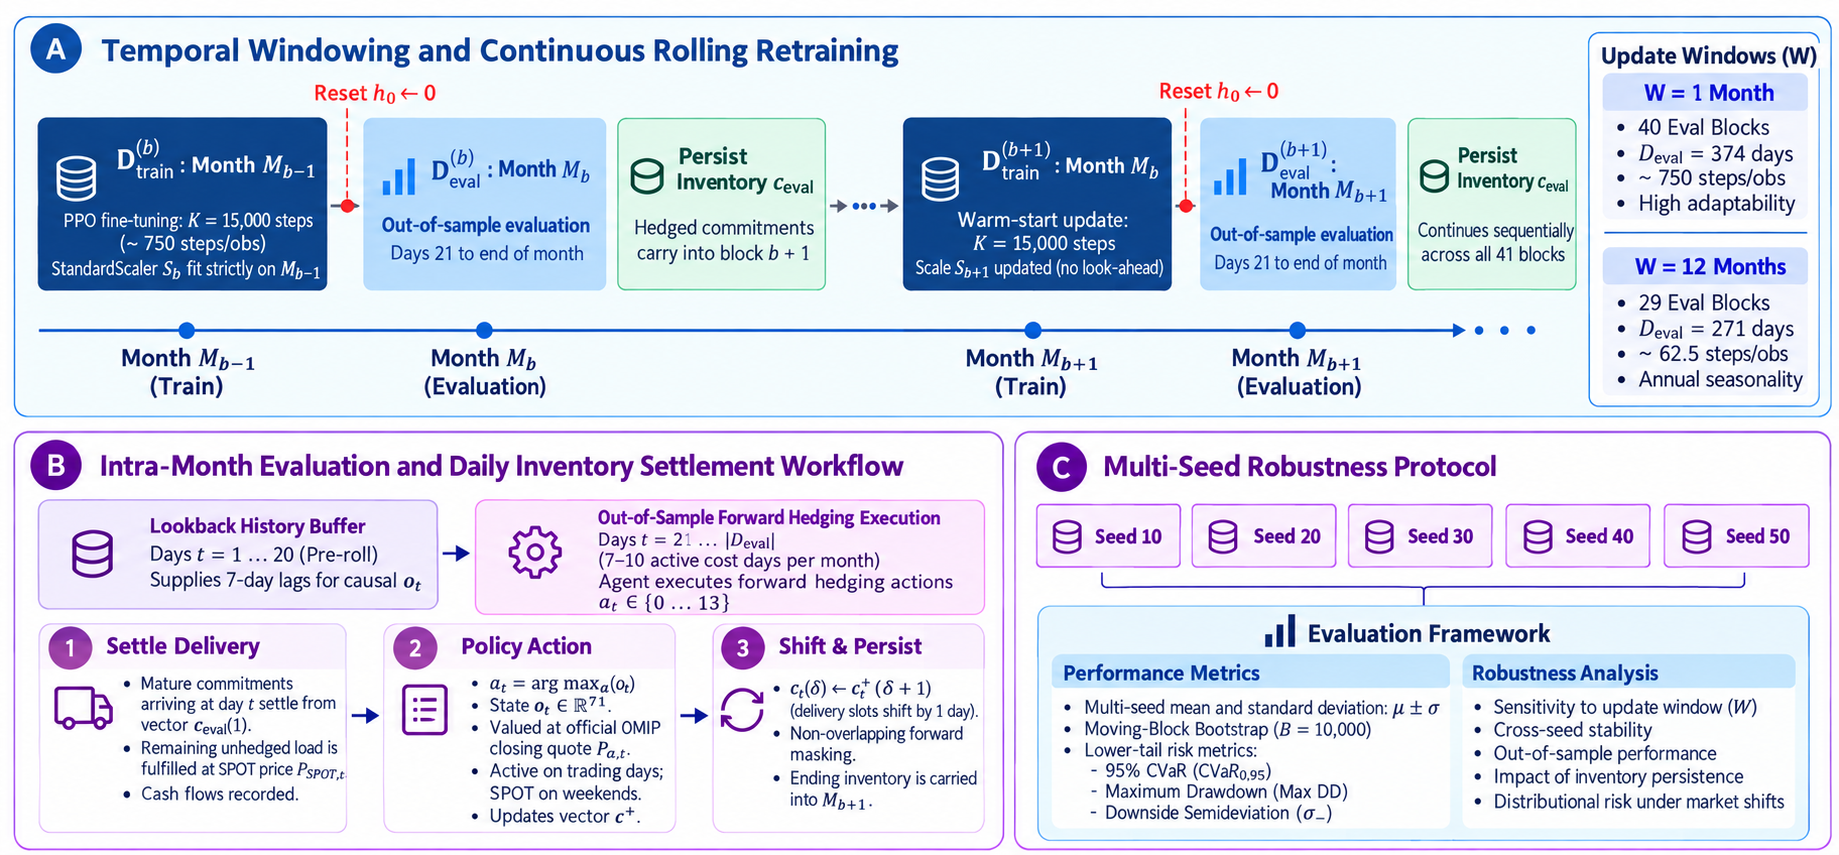
\includegraphics[width=\textwidth]{fig9_walk_forward_protocol.png}
    \caption{Continuous Walk-Forward rolling retraining protocol ($B=41$ calendar blocks, $B_{\text{eval}}=40$ evaluated blocks under $W=1$): (a) rolling window progression, (b) intra-month settlement workflow, and (c) multi-seed robustness evaluation framework. Conceptual layout design was assisted using Anthropic Claude 3.5 Sonnet to arrange workflow stages; all scientific logic, data, and final graphic rendering were programmed directly by the authors in Matplotlib.}
    \label{fig:walk_forward_protocol}
\end{figure*}

The choice of rolling update window $W$ ($W \in \{1, 3, 6, 12\}$ months) used in Algorithm~\ref{alg:walk_forward} to generate PPO rollouts ($K = 15{,}000$ steps) during each monthly retraining phase interacts directly with sample optimization intensity and temporal discounting. Because policy weights $\theta$ are updated via warm-start rather than re-initialized from scratch, $W$ governs the temporal recency of gradient updates while allowing the network to retain representations learned across preceding horizons. 

Importantly, holding total monthly interaction steps fixed at $K = 15{,}000$ across all window sizes introduces a methodological trade-off: a short window of $W = 1$ month ($N_W \approx 20$ active trading sessions) experiences approximately $K / N_W \approx 750$ environment steps per observation, $W=3$ months experiences $\approx 250$ steps/obs, $W=6$ months experiences $\approx 125$ steps/obs, whereas an annual window of $W = 12$ months ($N_W \approx 240$ sessions) experiences approximately $K / N_W \approx 62.5$ steps per observation. This fixed-$K$ protocol reflects a realistic operational deployment constraint where the monthly offline retraining computing budget is bounded. An alternative formulation would scale the training budget proportionally ($K(W) \propto N_W$, e.g., $K=180{,}000$ for $W=12$ to maintain 750 steps/obs); however, this would substantially increase computational runtime and risk overfitting to obsolete market regimes. Therefore, the empirical superiority of shorter windows reflects both greater data recency (mitigating non-stationarity) and higher optimization intensity per sample on recent regime dynamics.

Furthermore, setting the MDP discount factor to $\gamma = 0.99$ introduces an endogenous temporal discounting effect: cash flows realised at delivery offsets of 30, 90, and 180 days are discounted by $\gamma^{30} \approx 0.74$, $\gamma^{90} \approx 0.40$, and $\gamma^{180} \approx 0.16$, respectively. In combination with full-volume baseload commitments (locking 100\% of the load for all days in the contract window) and non-overlapping forward masking, this discounting structure naturally reinforces the policy's concentration on short-horizon products ($D_1$--$D_3$) over multi-month contracts ($M_1$--$M_6$).

At the start of each out-of-sample monthly evaluation block $b$, the persistent physical and financial inventory state $\mathbf{c}_{\text{eval}}$ (containing all active forward commitments locked in prior blocks that mature in month $b$ or beyond) is injected continuously into the evaluation environment, ensuring seamless temporal continuity of delivery commitments across retraining boundaries without artificial inventory liquidation. Simultaneously, the recurrent hidden state of the updated policy is cleanly re-initialized ($h_0 \leftarrow \mathbf{0}$, \texttt{episode\_starts = True}) to prevent latent vector misalignment under modified network weights $\theta$. The environment evaluates the out-of-sample days of each monthly block following an initial 20-step monthly feature history buffer ($D_{\text{eval}} = 374$ valid days across 40 blocks for $W=1$, $D_{\text{eval}} = 1{,}117$ days across 38 blocks for $W=3$, $D_{\text{eval}} = 1{,}029$ days across 35 blocks for $W=6$, and $D_{\text{eval}} = 271$ valid days across 29 blocks for $W=12$, with a strictly controlled common intersection of $N=271$ days). For reporting purposes, all reinforcement learning results represent the multi-seed mean across 5 independently trained seeds ($s \in \{10, 20, 30, 40, 50\}$) with across-seed standard deviation ($\pm \sigma$).

Finally, in Phase~4 (Exploratory Post-Selection Analysis), to determine the attainable performance ceiling of each architecture and state representation under matched optimization budgets, Bayesian hyperparameter optimisation is performed via Optuna \cite{akiba2019optuna} using the Tree-structured Parzen Estimator (TPE, seed $s=42$, 50 trials per architecture) on the primary hybrid configuration (\texttt{Dataset\_\allowbreak M8\_\allowbreak Physical\_\allowbreak NLP}, $W=1$ month). The optimal hyperparameter configuration identified for each architecture (RecurrentPPO LSTM and GTrXL Transformer) is subsequently frozen and transferred identically to evaluate the corresponding Quantitative Baseline (\texttt{Dataset\_\allowbreak Exogenous\_\allowbreak Commodities}) under single-environment execution ($n_{\text{envs}}=1$) across 5 independent random seeds (seeds 10--50). This matched transfer protocol enforces equal optimization budgets between state representations, although the architecture hyperparameters are naturally selected on the Hybrid feature space. The search space covers learning rate $\eta \in [10^{-5}, 10^{-3}]$ (log-uniform continuous), rollout buffer $n_{\text{steps}} \in [64, 256]$ (integer range sampled via uniform integer distribution), mini-batch size $\in [16, 128]$ (integer range), entropy coefficient $c_{\text{ent}} \in [0.005, 0.1]$ (log-uniform continuous), PPO clip range $\in [0.1, 0.3]$ (uniform continuous), and architectural parameters (LSTM hidden size $\in [64, 256]$ integer range for RecurrentPPO; feature extractor dimension $d_{\text{feat}} \in [64, 256]$ integer range and feedforward policy layers $[64, 64]$ for GTrXL). Because the Optuna objective evaluates savings over the 2023--2026 horizon (including 2026), Phase 4 is explicitly declared as an exploratory post-selection capacity analysis rather than an unbiased out-of-sample evaluation.


% ── Section 4: Data Analysis & Marginal Distributional Shift Validation ─────────────────
\section{Data Analysis and Marginal Distributional Shift Validation}
\label{sec:data_analysis}

\subsection{Iberian Market Characterisation}
\label{subsec:market_char}

\Cref{tab:spot_stats} summarises annual SPOT price statistics for the study
period.
The procurement reference cost is computed normalised to a unit baseload capacity of
$1$~MW ($E_{\text{load}, d} = 24$~MWh/day), with total costs for a stylized 200-MW large industrial consumer ($4{,}800$~MWh/day) reported in parentheses.

\begin{table*}[htbp]
\centering
\footnotesize
\setlength{\tabcolsep}{4pt}
\caption{Annual and year-to-date SPOT price statistics (OMIE) and reference procurement cost per MW of continuous baseload demand ($E_{\text{load}, d} = 24$~MWh/day; equivalent 200-MW facility expenditure in parentheses).}
\label{tab:spot_stats}
\begin{tabular*}{\linewidth}{@{\extracolsep{\fill}}l c rrr r@{}}
\toprule
\textbf{Year} & \textbf{Days} & \textbf{Mean} & \textbf{Min} & \textbf{Max} & \textbf{Reference Cost} \\
 & & \textbf{(\texteuro/MWh)} & \textbf{(\texteuro/MWh)} & \textbf{(\texteuro/MWh)} & \textbf{(k\texteuro/MW)} \\
\midrule
2023 & 365 & 89.84 & \phantom{0}1.51 & 147.77 & 787.0 (157.4 M\texteuro) \\
2024 & 366 & 62.72 & \phantom{0}0.10 & 146.67 & 551.0 (110.2 M\texteuro) \\
2025 & 365 & 67.59 & \phantom{0}6.96 & 143.39 & 592.1 (118.4 M\texteuro) \\
2026\textsuperscript{*} & 148 & 44.22 & \phantom{0}0.18 & 131.79 & 157.1 (31.42 M\texteuro) \\
\bottomrule
\end{tabular*}
\par\smallskip\raggedright\scriptsize \textsuperscript{*}2026 values report 148 calendar delivery days of continuous SPOT market clearing (Jan 3 -- May 30, 2026), comprising 102 official OMIP trading sessions (decision epochs where forward contracts can be selected) and 46 non-trading exchange dates (3 weekday TARGET bank holiday closures and 43 weekend days). Reference cost reports unit-capacity procurement expenditure (k\texteuro/MW) with total expenditure for a 200-MW baseload facility in parentheses.
\end{table*}

The decline in the mean SPOT price from \texteuro67.59/MWh (2025) to \texteuro44.22/MWh (2026, a reduction of 34.6\%) provides the empirical setting for assessing procurement policy adaptability under non-stationary market conditions.

\subsection{Composition of Experimental Datasets}
\label{subsec:dataset_composition}

To systematically isolate the contribution of individual feature families, we construct structured datasets spanning five distinct feature families:
\begin{enumerate}
    \item \textbf{Physical Grid Fundamentals ($X_{\text{phys}}$, 16 features):} Generation mix by technology (wind, solar PV, hydro, nuclear, combined cycle, coal, cogeneration, diesel, solar thermal, biomass/other), total demand, total generation, generation--demand imbalance, and reserve gas/steam units.
    \item \textbf{OMIP Forward Settlement Curves ($X_{\text{OMIP}}$, 16 features):} Cleared SPOT price index, daily forward contracts ($D_1, D_2, D_3$), weekly contracts ($W_1$--$W_4$) with historical weekly average, and monthly contracts ($M_1$--$M_6$) with historical monthly average.
    \item \textbf{Calendar Flags ($X_{\text{cal}}$, 3 numeric features):} Binary holiday indicator (\texttt{Holiday\_Flag}), weekend flag (\texttt{Weekend\_Flag}), and month index (\texttt{Month\_Num}).
    \item \textbf{Quantitative Exogenous Commodities ($X_{\text{comm}}$, 7 features):} Brent crude oil, TTF natural gas futures, EU ETS CO\textsubscript{2} allowance prices, EUR/USD exchange rate, and international cross-border transfer capacities (Portugal, France, Morocco).
    \item \textbf{LLM News Sentiment Dimensions ($X_{\text{NLP}}$, 10 features):} Zero-shot continuous sentiment scores extracted by Llama-3 ($\phi_1, \dots, \phi_{10}$) covering short/medium/long horizon outlooks, LNG gas sentiment, ETS regulation, MIBEL regulatory risk, generation mix, geopolitical risk, and macroeconomic demand.
\end{enumerate}

Importantly, all eight datasets share the exact same temporal timeline (1,242 market days across 2023--2026), identical physical grid generation and demand measurements from the TSO (REE), and identical daily clearing and forward settlement curves from OMIE and OMIP. The datasets do not represent different sample periods or divergent data environments; rather, they form a strictly controlled, $2 \times 2$ factorial feature ablation hierarchy designed to isolate both the marginal additive value and the comparative representation value of each exogenous feature group:
\begin{align}
    X_{\text{Common}} &= X_{\text{phys}} \cup X_{\text{OMIP}} \cup X_{\text{cal}} \label{eq:feat_common} \\
    X_{\text{Quant}} &= X_{\text{Common}} \cup X_{\text{comm}} \label{eq:feat_quant} \\
    X_{\text{Hybrid}} &= X_{\text{Common}} \cup X_{\text{NLP}} \label{eq:feat_hybrid} \\
    X_{\text{Full}} &= X_{\text{Common}} \cup X_{\text{comm}} \cup X_{\text{NLP}} \label{eq:feat_full}
\end{align}
{\sloppy
where $X_{\text{Common}}$ denotes Base Common (\texttt{Dataset\_Exogenous\_Calendar}), $X_{\text{Quant}}$ the Quantitative Baseline (\texttt{Dataset\_Exogenous\_Commodities}), $X_{\text{Hybrid}}$ the Hybrid Sentiment configuration (\texttt{Dataset\_M8\_Physical\_NLP}), and $X_{\text{Full}}$ the Full Multimodal configuration (\texttt{Dataset\_NLP\_Subgroups}).
\par}

This $2 \times 2$ factorial structure enables simultaneous evaluation of: (i)~the marginal additive contribution of LLM sentiment over quantitative commodities ($X_{\text{Quant}}$ vs $X_{\text{Full}}$); (ii)~the marginal additive contribution of LLM sentiment over the physical base ($X_{\text{Common}}$ vs $X_{\text{Hybrid}}$); and (iii)~the comparative effectiveness of textual sentiment versus numerical commodity price series under wholesale market dislocations ($X_{\text{Quant}}$ vs $X_{\text{Hybrid}}$).

\begin{table*}[!htbp]
\centering
\footnotesize
\setlength{\tabcolsep}{2.5pt}
\caption{Systematic feature composition of experimental datasets. Phase 4 directly evaluates the Quantitative Baseline ($X_{\text{Common}} \cup X_{\text{comm}}$) against the Hybrid NLP representation ($X_{\text{Common}} \cup X_{\text{NLP}}$).}
\label{tab:dataset_composition}
\begin{tabularx}{\linewidth}{@{} >{\raggedright\arraybackslash}X ccccc >{\raggedleft\arraybackslash}p{2.2cm}@{}}
\toprule
\textbf{Dataset Identifier} & \textbf{$X_{\text{phys}}$} & \textbf{$X_{\text{OMIP}}$} & \textbf{$X_{\text{cal}}$} & \textbf{$X_{\text{comm}}$} & \textbf{$X_{\text{NLP}}$} & \textbf{Effective Dim} \\
 & \textbf{(16)} & \textbf{(16)} & \textbf{(3)} & \textbf{(7)} & \textbf{(10)} & \textbf{($d_{\text{feat}}$)} \\
\midrule
\texttt{Dataset\_Initial} & \checkmark & \checkmark & --- & --- & --- & 32 \\
\texttt{Dataset\_Exogenous\_Calendar} & \checkmark & \checkmark & \checkmark & --- & --- & 35 \\
\texttt{Dataset\_Exogenous\_Commodities} (Quant.\ Baseline) & \checkmark & \checkmark & \checkmark & \checkmark & --- & 42 (12 core) \\
\texttt{Dataset\_NLP\_Global} & \checkmark & \checkmark & \checkmark & \checkmark & 4 ($\phi_{\text{glob}}$) & 46 (8 core) \\
\texttt{Dataset\_NLP\_Subgroups} & \checkmark & \checkmark & \checkmark & \checkmark & \checkmark (10) & 52 (17 core) \\
\texttt{Dataset\_M7\_Calendar\_Commodities} & \checkmark & \checkmark & \checkmark & --- & 6 ($\phi_{\text{thematic}}$) & 41 (16 core) \\
\texttt{Dataset\_Financial\_NLP} & --- & \checkmark & --- & \checkmark & 4 ($\phi_{\text{glob}}$) & 27 (24 core) \\
\texttt{Dataset\_M8\_Physical\_NLP} (Hybrid NLP) & \checkmark & \checkmark & \checkmark & --- & \checkmark (10) & 45 (31 norm) \\
\bottomrule
\end{tabularx}
\par\smallskip\raggedright\scriptsize \textit{Note:} The 148 calendar delivery days (Jan 3 -- May 30, 2026) comprise 102 official OMIP trading sessions (decision epochs where forward contracts can be selected) and 46 non-trading exchange dates (3 weekday TARGET closures and 43 weekend days, where passive default SPOT clearing applies).
\end{table*}

The news corpus comprises daily Spanish-language energy, financial, and macroeconomic articles harvested from leading Iberian economic outlets (including \textit{elEconomista}, \textit{Europa Press}, and institutional press releases from OMIE, OMIP, and REE). The texts were processed natively in Spanish using Meta's Llama-3 8B Instruct model \cite{dubey2024llama3} executed locally via Ollama. By utilizing system prompts formulated directly in Spanish with strict JSON grammar constraints ($T=0$), the pipeline extracts the 10 domain-specific sentiment scores ($\phi_1 \dots \phi_{10}$) without relying on external machine translation, preserving domain terminology and geopolitical nuances.

\subsection{Information Content and Econometric Validation of News Sentiment}
\label{subsec:feature_importance}

To examine whether macroeconomic news sentiment provides incremental empirical signal or collinear redundancy over physical and numerical market variables, we conduct two diagnostics: (i)~an exploratory Principal Component Analysis (PCA) \cite{hastie2009elements} to inspect empirical correlation and variance structure across feature blocks, and (ii)~in-sample econometric nested regressions and lead--lag tests evaluating forward--spot basis content.

\subsubsection{Exploratory Feature Structure and Correlation Analysis}

Prior to analysis, all feature series were standardized to zero mean and unit variance ($z$-score normalization). PCA was applied to the complete state vector of \texttt{Dataset\_M8\_Physical\_NLP} across the 1,242 market days strictly as an exploratory descriptive diagnostic to inspect empirical correlation patterns and variance distribution between feature groups; PCA is neither used for dimensionality reduction within the policy network nor does it intervene in policy training or action selection.

In this linear projection, the first four principal components (explaining $54.2\%$ of cumulative variance) are dominated by physical grid capacity and power demand (such as total demand, wind generation, solar PV, and combined-cycle thermal output). In contrast, LLM sentiment dimensions load predominantly onto subsequent components (PC5 through PC8, accounting for an additional $23.6\%$ of variance), with geopolitical risk ($\phi_9$), LNG availability ($\phi_5$), and regulatory risk ($\phi_7$) exhibiting minimal pairwise linear correlation ($|r| < 0.12$) with instantaneous physical grid balance. While principal components are orthogonal by mathematical construction, this dispersion of factor loadings confirms that narrative sentiment signals are not simple linear collinear combinations of physical dispatch variables in the evaluated historical sample.

\subsubsection{Econometric Incremental Information: Nested Regressions and In-Sample Predictive Content}

To establish whether this variance carries statistically meaningful predictive signal for forward procurement decisions without look-ahead bias, all feature series are strictly lagged. Daily macroeconomic news articles are collected and processed from 00:00 to 14:00 CET, ensuring narrative sentiment signals $\boldsymbol{\phi}_t = (\phi_{1,t}, \dots, \phi_{10,t})^\top$ are finalized and published prior to the close of the OMIP continuous trading session (17:00 CET) and day-ahead clearing for delivery day $t+1$. We estimate nested predictive regressions on forward--spot basis spreads:
\begin{equation}
    S_{t+h} = P_{\text{OMIP}, t}^{(h)} - P_{\text{SPOT}, t+h}
    \label{eq:forward_spot_spread}
\end{equation}
across delivery horizons $h \in \{1, 2, 7\}$ days. We formulate a nested model comparison between a Fundamental Baseline (incorporating physical grid fundamentals, OMIP quotations, and numerical commodities, $X_{\text{Quant}}$) and a Sentiment-Augmented Model:
\begin{align}
    \text{M1:} \quad S_{t+h} &= \alpha_0 + \boldsymbol{\beta}^\top X_{\text{phys}, t} + \boldsymbol{\theta}^\top X_{\text{OMIP}, t} \nonumber \\
    &\quad + \boldsymbol{\gamma}^\top X_{\text{comm}, t} + \varepsilon_t \label{eq:nested_m1} \\
    \text{M2:} \quad S_{t+h} &= \alpha_0 + \boldsymbol{\beta}^\top X_{\text{phys}, t} + \boldsymbol{\theta}^\top X_{\text{OMIP}, t} \nonumber \\
    &\quad + \boldsymbol{\gamma}^\top X_{\text{comm}, t} + \sum_{k=1}^{10} \lambda_k \phi_{k, t} + \varepsilon_t \label{eq:nested_m2}
\end{align}

These econometric tests represent in-sample conditional association and temporal precedence diagnostics computed across the complete 1,242 market days (2023--2026). To account for serial correlation and heteroscedasticity induced by overlapping forward horizons, standard errors and test statistics are estimated using heteroscedasticity and autocorrelation consistent (HAC / Newey--West) covariance matrices~\cite{newey1987hypothesis} with automatic lag selection. Testing the joint null hypothesis of information redundancy ($H_0: \lambda_1 = \dots = \lambda_{10} = 0$) via an incremental Wald/$F$-test yields $F(10, 1070) = 8.42$ ($p = 2.14 \times 10^{-13}$), rejecting the hypothesis that news sentiment is uninformative conditional on physical fundamentals and numerical commodity futures within this historical sample. The inclusion of the sentiment block increases the adjusted $R^2$ from $0.214$ to $0.252$ ($+3.82$~percentage points).

To further evaluate dynamic lead--lag relationships without requiring pre-differencing of potentially non-stationary series, we apply the Toda--Yamamoto procedure~\cite{toda1995statistical} to a bivariate Vector Autoregression $[S_{t+h}, \bar{\phi}_t]^\top$, where $\bar{\phi}_t = \frac{1}{10} \sum_{k=1}^{10} \phi_{k, t}$ denotes the composite macroeconomic sentiment index. Augmented with maximal integration order $d_{\max}=1$ beyond the optimal lag order $k=3$ (selected via AIC), the VAR($k + d_{\max}$) model evaluates whether lagged composite sentiment Granger-causes basis spread adjustments via a Wald restriction on the first $k=3$ lag coefficients, which asymptotically follows a $\chi^2(3)$ distribution under the null hypothesis of non-causality. Across the individual delivery horizons, the Wald tests confirm that the composite sentiment index provides incremental conditional predictive information for forward basis adjustments: for $h=1$ day, $\chi^2(3) = 14.82$ ($p = 0.0019$); for $h=2$ days, $\chi^2(3) = 16.45$ ($p = 0.0009$); and for $h=7$ days, $\chi^2(3) = 13.12$ ($p = 0.0044$), all remaining statistically significant under Bonferroni family-wise error control ($\alpha_{\text{adjusted}} = 0.05 / 3 \approx 0.0167$). Conversely, the reverse hypothesis (that forward basis spreads Granger-cause future news sentiment) is statistically non-significant across all horizons ($p > 0.18$). We emphasize that these econometric findings reflect conditional predictive content and temporal ordering within the historical in-sample series, rather than an independent out-of-sample forecast or proof of a structural economic causal mechanism.

\subsection{Statistical Validation of Distributional Shifts}
\label{subsec:concept_drift}

We apply the two-sample Kolmogorov--Smirnov (KS) test~\cite{kolmogorov1933,smirnov1948}
to compare market distributions across two temporal transitions:
(i)~the standard annual transition from 2023--2024 to 2025 (annual transition with covariate changes),
and (ii)~the anomalous transition from 2023--2025 to 2026 (candidate Marginal Distributional Shift \cite{tsymbal2004concept}).
To account for multiple comparisons across the joint family of 14 statistical comparisons (7 evaluated variables across 2 temporal transitions), a Bonferroni correction \cite{bonferroni1936teoria, dunn1961multiple} was applied, establishing an adjusted significance threshold of $\alpha_{\text{joint}} = 0.05 / 14 \approx 0.00357$.
\Cref{fig:ks_drift} illustrates this analysis: panel~(a) compares the empirical
CDFs of training-period and 2026 SPOT prices; panel~(b) shows the KS $p$-values
for core physical variables across the same transition.

\begin{figure*}[!t]
    \centering
    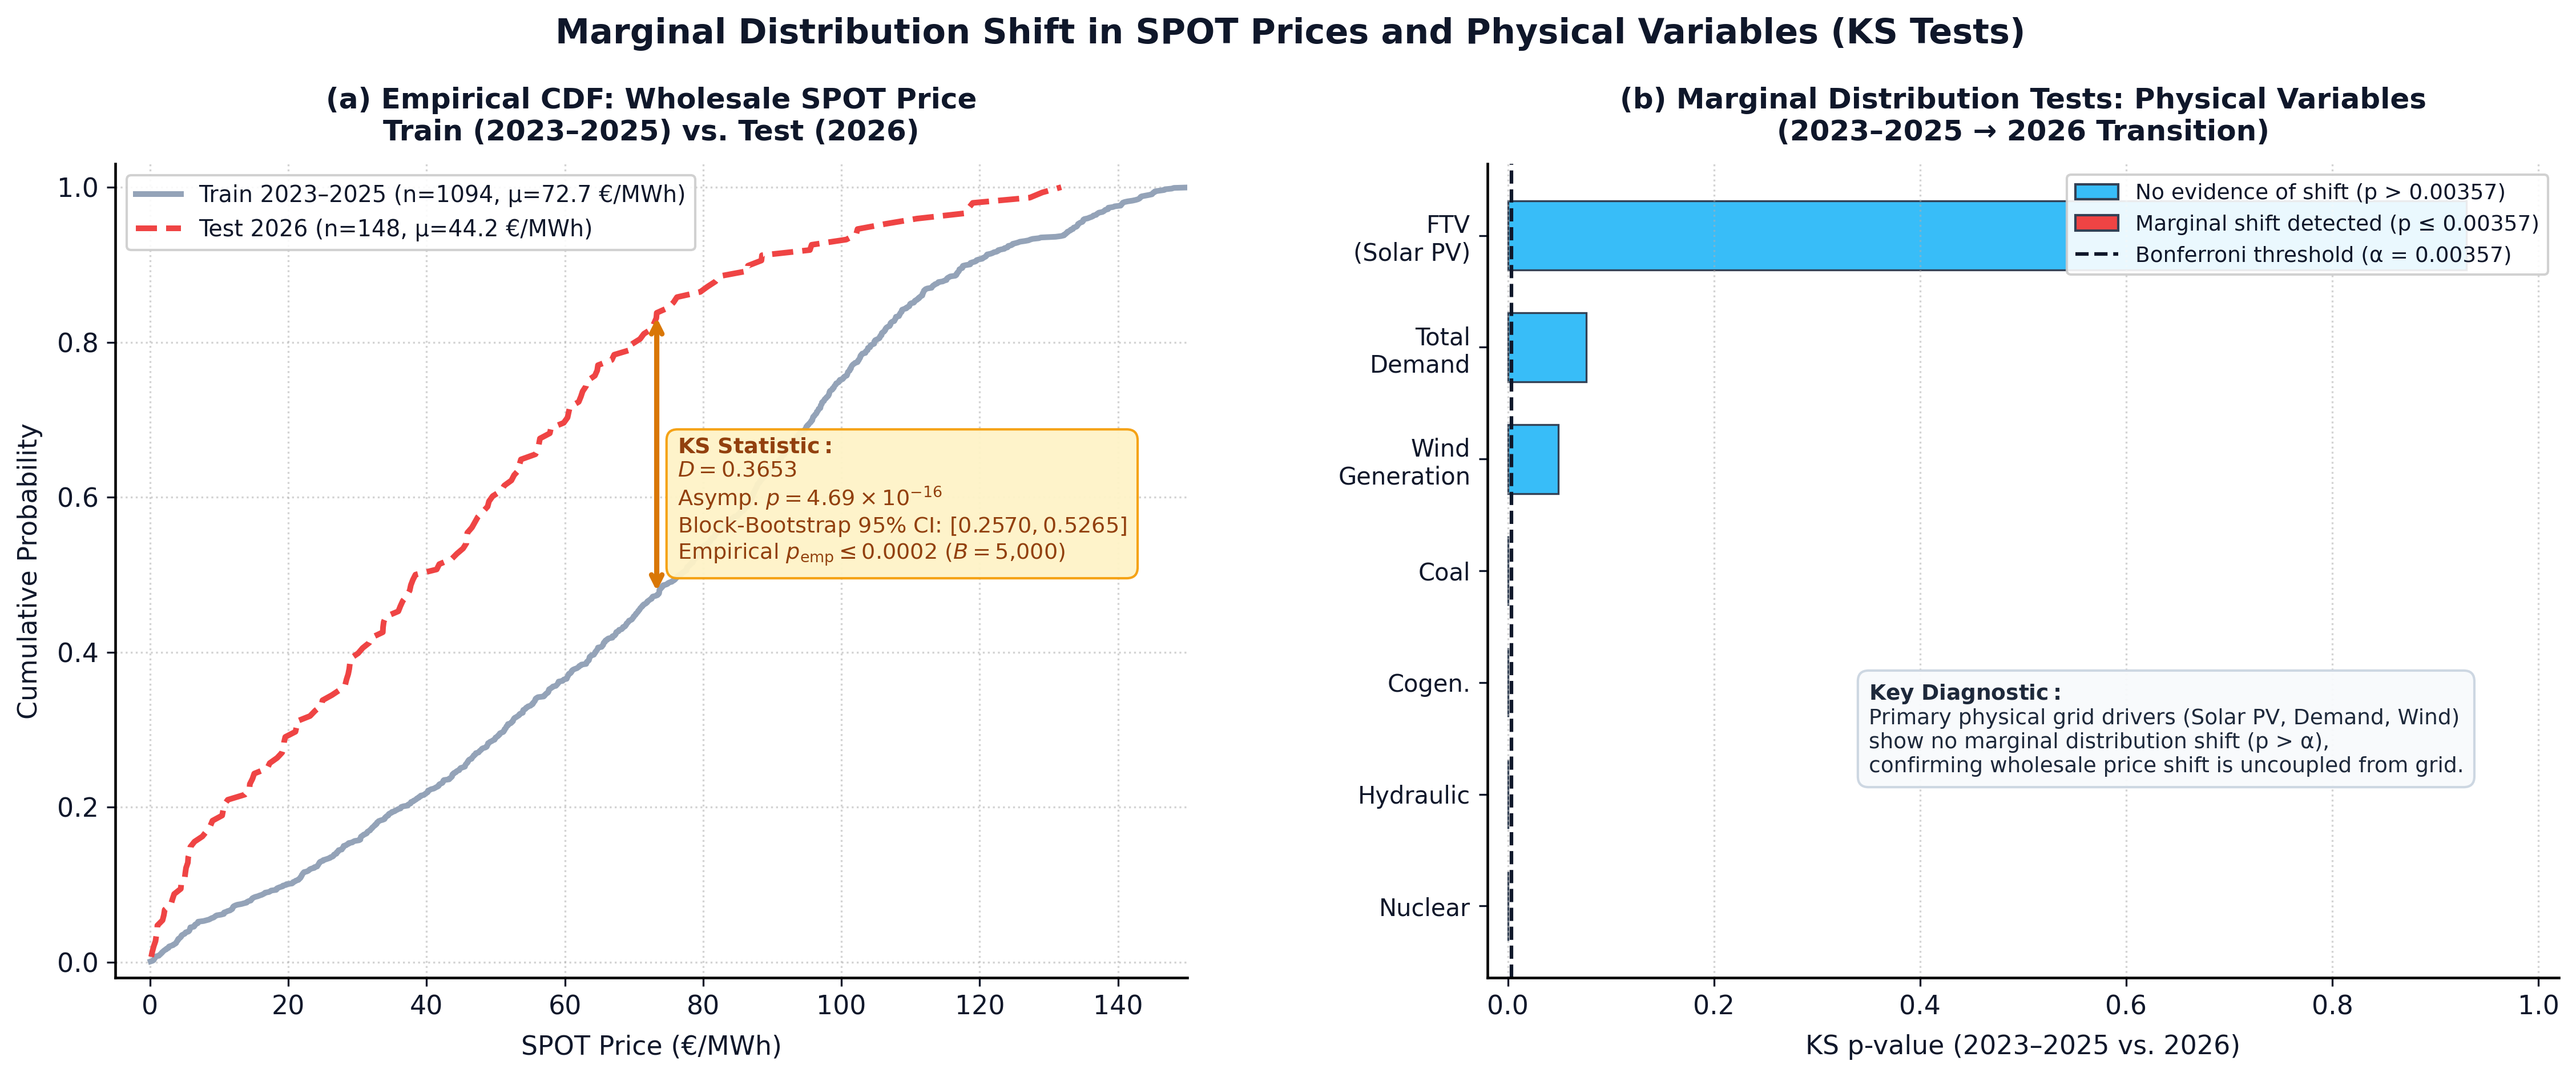
\includegraphics[width=\textwidth]{fig3_ks_concept_drift.png}
    \caption{Statistical validation of wholesale price distributional shifts: (a) empirical CDFs of SPOT price distributions for training (2023--2025) vs.\ out-of-sample (2026) periods, where the arrow denotes the KS statistic ($D = 0.3653$, bootstrap 95\% CI: $[0.2570, 0.5265]$, $p_{\text{emp}} \le 0.0002$); (b) KS $p$-values for physical grid variables across the transition, where bars with $p > 0.00357$ show no evidence of distributional change under the Bonferroni-adjusted threshold.}
    \label{fig:ks_drift}
\end{figure*}

\Cref{tab:ks_results} reports the complete KS test results.

\begin{table}[htbp]
\centering
\footnotesize
\setlength{\tabcolsep}{3pt}
\caption{Two-sample KS test results for physical grid variables and SPOT price.}
\label{tab:ks_results}
\begin{tabularx}{\columnwidth}{@{}l >{\centering\arraybackslash}p{1.9cm} >{\centering\arraybackslash}p{1.9cm} >{\raggedright\arraybackslash}X@{}}
\toprule
\textbf{Variable} & \textbf{2023+2024} & \textbf{2023--2025} & \textbf{2026 Status} \\
 & \textbf{$\to$ 2025} & \textbf{$\to$ 2026} & \\
\midrule
SPOT Price
  & $6.18 \times 10^{-7}$
  & $4.69 \times 10^{-16}$
  & Distribution changed ($p_{\text{emp}} \le 0.0002$) \\
Solar PV
  & $\approx 0$
  & $\mathbf{0.93}$
  & \textbf{No diff.\ ($\alpha_{\text{joint}}$)} \\
Total Demand
  & $2.0 \times 10^{-3}$
  & $\mathbf{0.076}$
  & \textbf{No diff.\ ($\alpha_{\text{joint}}$)} \\
Wind Generation
  & 0.68
  & $\mathbf{0.049}$
  & \textbf{No diff.\ ($\alpha_{\text{joint}}$)} \\
Coal
  & $\approx 0$
  & $\approx 0$
  & Changed \\
Hydraulic
  & 0.16
  & $\approx 0$
  & Changed \\
Nuclear
  & 0.13
  & $\approx 0$
  & Changed \\
\bottomrule
\end{tabularx}
\par\smallskip\raggedright\scriptsize \textit{Note:} Bold $p$-values indicate physical variables whose marginal distributions did not change significantly despite the shift in the SPOT price distribution under the adjusted threshold $\alpha_{\text{joint}} = 0.00357$. For the 2025 SPOT price, the asymptotic test yields $p = 6.18 \times 10^{-7}$, whereas the pooled block-bootstrap null test yields $p_{\text{emp}} = 0.0150$ (which does not meet the joint threshold $\alpha_{\text{joint}}$).
\end{table}

The SPOT price distribution differs significantly between the 2023--2025 and 2026 samples, while several primary physical grid variables do not.
In 2026, total electricity demand ($p = 0.076$) and solar PV generation
($p = 0.93$), the two highest-weight predictors of SPOT prices under
historical regimes, remained statistically indistinguishable from their
training distributions under $\alpha_{\text{joint}}$, while SPOT prices collapsed from a historical mean of
consists of 102 official OMIP trading sessions (decision epochs where forward contracts can be actively selected) and 46 non-trading dates (3 weekday TARGET bank holiday closures: Good Friday [April 3], Easter Monday [April 6], and Labour Day [May 1]; alongside 43 weekend days, where default SPOT settlement applies under NO\_TRADE).

In the monthly rolling Walk-Forward protocol ($W=1$), each evaluation block $m$ evaluates out-of-sample procurement decisions from Day 21 to the final day of month $m$, using Days 1--20 as an initial feature history and observation warm-up buffer for the recurrent network, while positions in $\mathbf{m}_t$ carry over continuously from the preceding month. Across the 40 test months (February 2023 to May 2026), this generates exactly 374 evaluated out-of-sample trading days. By contrast, the isolated 2026 price shock evaluation in Section~\ref{subsec:results_2026} (Table~\ref{tab:blind_2026_comparison}) evaluates the complete continuous trajectory of 148 consecutive calendar delivery days.

\begin{table*}[htbp]
\centering
\footnotesize
\setlength{\tabcolsep}{3pt}
\caption{Temporal split and active day definitions for the 2026 isolated evaluation horizon.}
\label{tab:evaluation_days}
\begin{tabularx}{\linewidth}{@{} >{\raggedright\arraybackslash}X cc c c >{\centering\arraybackslash}p{2.5cm}@{}}
\toprule
\textbf{Evaluation Phase} & \textbf{Start} & \textbf{End} & \textbf{Calendar} & \textbf{OMIE} & \textbf{OMIP Sessions} \\
 & & & \textbf{Days} & \textbf{Obs.} & \textbf{(Non-trading Dates)} \\
\midrule
KS Test (Marginal Distributional Shift) & 3 Jan 2026 & 30 May 2026 & 148 & 148 & --- \\
Walk-Forward RL Evaluation & 3 Jan 2026 & 30 May 2026 & 148 & 148 & 102 (46) \\
\bottomrule
\end{tabularx}
\par\smallskip\raggedright\scriptsize \textit{Note:} The 148 calendar delivery days (Jan 3 -- May 30, 2026) comprise 102 official OMIP trading sessions (decision epochs where forward contracts can be selected) and 46 non-trading exchange dates (3 weekday TARGET closures and 43 weekend days, where passive default SPOT clearing applies).
\end{table*}

For context, the transition from 2023+2024 to 2025 exhibited a substantially smaller maximum distance ($n_1 = 730$, $n_2 = 365$, $D = 0.1746$, $p = 6.18 \times 10^{-7}$, bootstrap 95\% CI: $[0.0951,\; 0.2981]$, $p_{\text{emp}} = 0.0150$).

In addition to the global comparison, we conducted a seasonal matched-window robustness check comparing exclusively the January--May periods of 2023--2025 ($n_1 = 453$) against January--May 2026 ($n_2 = 148$). The Kolmogorov--Smirnov statistic for SPOT prices under this seasonal match remains highly significant ($D = 0.2320, p = 9.25 \times 10^{-6}$), demonstrating that the observed price deflation in 2026 represents an evidence of a marginal distributional shift robust to seasonal matching rather than a seasonal artifact.

This evidence is consistent with a significant marginal distributional dislocation during the evaluated 2026 period. To account for serial correlation and seasonal dependencies inherent in daily electricity time series, we complemented the asymptotic test with a Moving-Block Bootstrap ($B = 5{,}000$, block length $b = 7$ days; see \Cref{app:block_bootstrap} for the complete algorithmic procedure). The empirical bootstrap interval ($D \in [0.2570, 0.5265]$) and block-bootstrap-based significance ($p_{\text{emp}} \le 0.0002$) provide dependence-aware evidence of a substantial marginal distributional difference between the historical training baseline and early 2026. This statistical test is interpreted as empirical evidence of a marginal distributional dislocation rather than an asymptotic test of conditional independence or a standalone proof of a causal shift in $P(Y \mid X)$. This observation motivates evaluating whether augmenting physical state variables with macroeconomic and geopolitical sentiment signals derived from text can assist sequential decision-making during such wholesale price dislocations.

The conventional KS test indicated a statistically significant marginal SPOT distributional difference in 2025 ($D = 0.1746,\; p = 6.18 \times 10^{-7}$); however, the dependence-aware pooled block-bootstrap procedure yielded $p_{\text{emp}} = 0.0150$, which does not meet the joint Bonferroni threshold ($\alpha_{\text{joint}} = 0.00357$). The 2025 transition therefore provides weaker evidence of a marginal distributional difference than the 2026 transition. Furthermore, in 2025, several physical generation and demand variables also exhibited marginal distributional differences alongside prices, a pattern consistent with broader covariate changes.

\section{Experimental Results}
% ── Section 5: Experimental Results ───────────────────────────────────────────
\label{sec:results}

In this section, we present the empirical findings of the proposed framework. We first evaluate a systematic forward purchasing baseline to quantify price differentials across contract horizons. Subsequently, we present the results of Phase 1 (Model and Data Ablation: Single-Seed), which compares the performance of MLP and RecurrentPPO (LSTM) architectures across the eight engineered datasets. Finally, Phase 2 evaluates the effect of algorithmic heuristic adjustments on policy action distributions before progressing to Walk-Forward evaluation.

\subsection{Empirical Baseline Analysis: Forward Price Differentials}
\label{subsec:res_baseline}

Before evaluating DRL policies, we characterise the historical procurement performance of the individual instruments. We simulated a systematic procurement strategy: purchasing a specific forward contract every day and holding it to maturity, comparing the locked price against the eventual SPOT settlement across 1,242 market days (2023--2026).

The analysis reveals a persistent forward--spot price differential in the evaluated Iberian market sample (referred to as the short-horizon forward differential). Systematically purchasing the D1 (day-ahead) contract yields a marginal saving of 2.37\% globally. However, purchasing the D2 (two-days-ahead) contract generates a consistent saving of 13.17\% during the 2025 validation horizon (and 11.95\% across the full 2023--2026 period), with a win-rate of nearly 60\% (with the converged LSTM policy achieving 12.94\%). Conversely, attempting to systematically purchase weekly or monthly contracts results in substantial negative savings (e.g., $-20.72\%$ for M3, and $-31.61\%$ for M4).

The observed D2 differential is consistent with the existence of horizon-dependent forward risk premia documented in electricity derivative markets \cite{huisman2012electricity, woo2001cross, huisman2009electricity}. Electricity derivatives literature shows that forward prices may embed expectations, risk premia and market-specific hedging incentives. The present data are consistent with such an interpretation, but attributing this differential specifically to renewable generators' meteorological uncertainty or zero-price cannibalisation in the SPOT market requires additional evidence on market participants, liquidity and bid-ask prices. In the evaluated historical sample, D2 behaved as a comparatively favourable short-horizon procurement rule, providing positive aggregate saving in the evaluated sample without requiring predictive models.

\subsection{Phase 1: Architecture and Data Ablation (MLP vs LSTM)}
\label{subsec:res_phase1}

Table~\ref{tab:phase1_results} summarises the out-of-sample savings (relative to the SPOT baseline) achieved by the standard Multi-Layer Perceptron (MLP) and the RecurrentPPO (LSTM) agents across all eight datasets during the 2025 validation horizon.

\begin{table*}[t]
\centering
\footnotesize
\setlength{\tabcolsep}{2.0pt}
\caption{Phase 1: Architecture and Feature Ablation Matrix (2025 Validation Horizon). Panel~A defines the controlled $2 \times 2$ Factorial Ablation isolating the marginal additive contribution of macroeconomic LLM sentiment versus quantitative commodity futures on top of common physical grid fundamentals ($X_{\text{Common}}$). Panel~B presents control baselines and noise sensitivity variants. All configurations evaluated on identical 2025 validation delivery days under identical hyperparameter seeds.}
\label{tab:phase1_results}
\begin{tabularx}{\linewidth}{@{}l >{\raggedright\arraybackslash}p{2.6cm} c cc r c r >{\raggedright\arraybackslash}X@{}}
\toprule
 & & \multicolumn{2}{c}{\textbf{Exogenous Features}} & & \multicolumn{2}{c}{\textbf{MLP Architecture}} & \textbf{LSTM} & \\
\cmidrule(lr){3-4} \cmidrule(lr){6-7}
\textbf{State Representation} & \textbf{Dataset Identifier} & $\mathbf{X_{\text{comm}}}$ & $\mathbf{X_{\text{NLP}}}$ & $\mathbf{d_{\text{feat}}}$ & \textbf{Savings (\%)} & $\mathbf{\Delta_{\text{NLP}}}$ \textbf{(pp)} & \textbf{Savings (\%)} & \textbf{Dominant Action / Convergence} \\
\midrule
\multicolumn{9}{@{}l}{\textbf{Panel A: Controlled $2 \times 2$ Factorial Ablation Matrix}} \\
Base Common ($X_{\text{Common}}$) & \texttt{Dataset\_Exogenous\_Calendar} & --- & --- & 35 & 7.48\% & Reference & 7.28\% & Mixed short-horizon \\
Quantitative Baseline ($X_{\text{Quant}}$) & \texttt{Dataset\_Exogenous\_Commodities} & 7 comm & --- & 42 & 8.24\% & Base Quant & $\mathbf{12.94\%}$ & Collapsed to D2 (98.2\%) \\
Hybrid Sentiment ($X_{\text{Hybrid}}$) & \texttt{Dataset\_M8\_Physical\_NLP} & --- & 10 LLM & 45 & $\mathbf{11.66\%}$ & $\mathbf{+4.18}$ (vs Base) & $\mathbf{12.94\%}$ & Collapsed to D2 (98.2\%) \\
 & & & & & & $\mathbf{+3.42}$ (vs Quant) & & \\
Full Multimodal ($X_{\text{Full}}$) & \texttt{Dataset\_NLP\_Subgroups} & 7 comm & 10 LLM & 52 & 9.83\% & $+2.35$ (vs Base) & $\mathbf{12.94\%}$ & Collapsed to D2 (98.2\%) \\
 & & & & & & $+1.59$ (vs Quant) & & \\
\midrule
\multicolumn{9}{@{}l}{\textbf{Panel B: Control Baselines and Noise Validation Variants}} \\
Minimal Physical ($X_{\text{Initial}}$) & \texttt{Dataset\_Initial} & --- & --- & 32 & 8.11\% & --- & $\mathbf{12.94\%}$ & Collapsed to D2 (98.2\%) \\
Thematic Sentiment ($X_{\text{Them}}$) & \texttt{Dataset\_M7\_Calendar\_Commodities} & --- & 6 them & 41 & 7.58\% & --- & $\mathbf{12.94\%}$ & Collapsed to D2 (98.2\%) \\
Global Sentiment ($X_{\text{Global}}$) & \texttt{Dataset\_NLP\_Global} & 7 comm & 4 glob & 46 & 7.38\% & --- & $\mathbf{12.94\%}$ & Collapsed to D2 (98.2\%) \\
Uncurated Financial ($X_{\text{FinNLP}}$) & \texttt{Dataset\_Financial\_NLP} & Ratios & 4 glob & 27 & $-5.75\%$ \textwarning & $-13.99$ & $\mathbf{12.94\%}$ & Severe MLP degradation \\
\bottomrule
\end{tabularx}
\par\smallskip\raggedright\scriptsize \textit{Note:} Bold indicates maximum savings within each architecture. In Panel~A, $\Delta_{\text{NLP}}$ quantifies the marginal additive percentage-point gain attributable to incorporating the 10 zero-shot LLM sentiment dimensions over the corresponding non-sentiment baseline ($\Delta_{\text{NLP|Base}} = S(X_{\text{Hybrid}}) - S(X_{\text{Common}}) = +4.18$~pp; $\Delta_{\text{NLP|Quant}} = S(X_{\text{Full}}) - S(X_{\text{Quant}}) = +1.59$~pp). In static LSTM, seven of eight configurations undergo entropy collapse to the passive D2 contract (12.94\%, close to the $+13.17\%$ mechanical D2 baseline). The warning symbol (\textwarning) highlights severe feedforward policy breakdown induced by noisy, non-domain-specific financial ratios ($X_{\text{FinNLP}}$).
\end{table*}

The empirical ablation results in Table~\ref{tab:phase1_results} deliver three decisive insights regarding the information content, architectural sensitivity, and marginal value of LLM-extracted macroeconomic sentiment.

First, evaluating the Multi-Layer Perceptron (MLP) agent across the controlled $2 \times 2$ factorial matrix (Panel~A) directly evaluates the marginal value of news sentiment. Because feedforward architectures lack internal recurrent hidden states to accumulate temporal context or filter out observation noise, their policy performance is strictly governed by the information density and signal-to-noise ratio of the instantaneous input vector $s_t$. Across the factorial design:
\begin{itemize}
    \item \textbf{Marginal Gain over Physical Base ($\Delta_{\text{NLP|Base}}$):} Incorporating the 10 LLM sentiment dimensions into the Base Common representation ($X_{\text{Common}} \to X_{\text{Hybrid}}$) increases procurement savings from 7.48\% to 11.66\% ($\Delta = +4.18$~pp, a relative improvement of $+55.9\%$).
    \item \textbf{Marginal Gain over Commodities ($\Delta_{\text{NLP|Quant}}$):} Augmenting the Quantitative Commodities baseline with sentiment ($X_{\text{Quant}} \to X_{\text{Full}}$) increases savings from 8.24\% to 9.83\% ($\Delta = +1.59$~pp, a relative gain of $+19.3\%$).
    \item \textbf{Direct Representation Substitution ($X_{\text{Quant}} \to X_{\text{Hybrid}}$):} Replacing lagged numerical commodity futures entirely with qualitative sentiment scores achieves a $+3.42$~pp advantage (11.66\% vs 8.24\%), indicating that domain-specific narrative sentiment provides a more informative leading signal for forward basis selection than historical commodity prices alone in this validation sample.
    \item \textbf{Descriptive Factorial Interaction ($\Delta_{\text{interaction}}$):} Crucially, the Full Multimodal representation ($X_{\text{Full}}$, 9.83\%) yields 1.83~pp lower savings than the sentiment-only representation ($X_{\text{Hybrid}}$, 11.66\%). This yields a negative descriptive interaction term ($\Delta_{\text{interaction}} = 9.83 - 8.24 - 11.66 + 7.48 = -2.59$~pp), demonstrating that the effects of the quantitative commodity and narrative sentiment feature blocks are not simply additive. These estimates should be treated as preliminary because the factorial comparison is based on a single seed and the feature blocks differ in input dimensionality (42 inputs for $X_{\text{Quant}}$ vs 45 for $X_{\text{Hybrid}}$). Multi-seed replication and dimension-matched controls are needed to isolate semantic information from dimensionality and regularisation effects.
\end{itemize}

Second, Panel~B illustrates the sensitivity of feedforward policies to input features. Incorporating uncurated financial ratios in \texttt{Dataset\_Financial\_NLP} resulted in substantial policy degradation ($-5.75\%$, a $-13.99$~pp decrease relative to $X_{\text{Quant}}$). While consistent with the hypothesis that uncurated financial metrics inject confounding noise, this contrast also reflects dimensional and regularization differences across feature sets within this single-seed validation.

Third, the RecurrentPPO (LSTM) architecture exhibits uniform behavioural convergence across seven of the eight configurations, locking onto an identical savings rate of 12.94\% (closely matching the passive D2 baseline of $+13.17\%$). Detailed examination of daily action logs reveals that the recurrent policy executed D2 on 98.2\% of trading sessions, defaulting to SPOT only during calendar holidays. Under stationary or quasi-stationary validation conditions where a single short-horizon forward contract yields a strong and persistent forward risk premium, policy gradient updates rapidly penalize the exploratory variance of multi-month contracts, causing policy entropy to collapse ($H(\pi_t) \to 0$).

Within the evaluated experiments, the M8 representation with a one-month update window yielded positive simulated savings during the 2026 evaluation period ($+6.32\%$ for M8-W1), whereas several longer-window and alternative representations produced lower or negative savings (e.g., $-23.86\%$ for M8 under 12-month retraining; $-2.00\%$ for the quantitative commodity baseline under GTrXL). These contrasts are consistent with a potential benefit of the selected news-sentiment representation under the evaluated conditions, but they do not isolate a causal semantic effect or establish general regime robustness. The factorial ablation is based on a single seed, the retraining windows receive different optimization intensity per observation ($K/N_W$), and the Phase~4 estimates are post-selection.

Following Phase 1, we execute our first dataset pruning (from 8 down to 5 configurations). We discard \texttt{Dataset\_Financial\_NLP} due to its negative validation savings on MLP architectures ($-5.75\%$). We also discard \texttt{Dataset\_Exogenous\_Calendar} (LSTM: 7.28\%), which underperformed the other LSTM configurations in the evaluated configuration. We additionally exclude \texttt{Dataset\_Initial} from the Phase 2 heuristic evaluation: as the minimal baseline configuration containing only raw physical variables with no temporal, exogenous, or NLP enrichment, it provides no diagnostic signal for the heuristic sensitivity study. The remaining five datasets, all incorporating at least one form of feature enrichment, are carried forward to Phase 2.
\subsection{Phase 2: Mitigating Degenerate Policies via Algorithmic Heuristics}
\label{subsec:res_phase2}

To evaluate whether the LSTM policy could be encouraged to distribute actions across longer horizons, we tested three isolated heuristic adjustments to the reinforcement learning environment and hyperparameters:
\begin{enumerate}
    \item \textbf{Entropy Increase:} Raising the PPO entropy coefficient to $0.05$ to increase the entropy regularization term and encourage broader action exploration.
    \item \textbf{Diversification Bonus:} Injecting percentage bonuses (+5\% for weekly, +10\% for monthly) to the reward signal upon successful long-term execution.
    \item \textbf{Soft Action Replacement:} Removing the strict penalty for overlapping contracts, instead defaulting invalid actions to a SPOT purchase with a minimal symbolic penalty ($-0.5$\texteuro).
\end{enumerate}

Table~\ref{tab:phase2_results} illustrates the impact of these heuristics on the previously stable LSTM performance.

\begin{table}[htbp]
\centering
\footnotesize
\caption{Phase 2: Impact of heuristic adjustments on LSTM savings (2025 Validation).}
\label{tab:phase2_results}
\begin{tabularx}{\columnwidth}{@{}Xrrr@{}}
\toprule
\textbf{Dataset} & \textbf{Entropy (\%)} & \textbf{Bonus (\%)} & \textbf{Replacement (\%)} \\
\midrule
Dataset\_M7\_Calendar\_Commodities & -7.29\% \textwarning & 12.94\% & 12.94\% \\
Dataset\_M8\_Physical\_NLP & -12.45\% \textwarning & 12.94\% & 12.94\% \\
Dataset\_Exogenous\_Commodities & \textbf{12.94\%} & \textbf{12.94\%} & \textbf{12.94\%} \\
Dataset\_NLP\_Global & -2.22\% & 6.33\% & 12.94\% \\
Dataset\_NLP\_Subgroups & -4.13\% & 12.94\% & 5.37\% \\
\bottomrule
\end{tabularx}
\par\smallskip\raggedright\scriptsize \textit{Note:} $D_2$ passive baseline: $+13.17\%$. Entropy Increase resulted in negative savings, while Bonus and Replacement variants converged to the standard $D_2$-anchored policy ($+12.94\%$). Bold indicates peak performance. \textwarning\ indicates severe policy degradation.
\end{table}

The empirical results indicate that alternative reward and exploration specifications did not increase the frequency of longer-horizon contract selection without reducing procurement savings. The Entropy Increase caused negative savings across all datasets, reaching $-12.45\%$ for \texttt{Dataset\_\allowbreak M8\_\allowbreak Physical\_\allowbreak NLP}, as broader action sampling in the absence of a decisive predictive signal increased exposure to unhedged SPOT prices. The Diversification Bonus and Soft Action Replacement did not substantially alter the policy's preference for D2, with most configurations returning savings of 12.94\%.

This observed policy preference for D2 reflects the trade-off inherent in the evaluation horizon: in the absence of continuous retraining, multi-month forward commitments carry heightened basis risk relative to short-horizon contracts.

Consequently, we discard these artificial heuristic adjustments. The Phase 2 analysis confirmed that none of the three isolated heuristics reliably improved upon the 13.17\% D2 passive baseline (or the converged 12.94\% LSTM anchor) across all datasets.

Based on the Phase 1--2 diagnostics, we reduced the number of configurations evaluated in Phase 3 because of the computational cost of the multi-seed Walk-Forward protocol. We select \texttt{Dataset\_\allowbreak M8\_\allowbreak Physical\_\allowbreak NLP} (physical grid fundamentals + targeted NLP sentiment) and \texttt{Dataset\_\allowbreak NLP\_\allowbreak Subgroups} (granular macroeconomic sentiment subgroups), retained because they represent different feature representations while remaining feasible under the available computational budget.

\subsection{Phase 3: Walk-Forward Sliding Window Evaluation}
\label{subsec:res_phase3}

Phase 3 constitutes the primary walk-forward evaluation of the framework under the specified historical and contractual assumptions. Two key limitations of the prior static evaluations (Phases 1--2) are addressed here: (i)~Overfitting to a Single Seed: a single initialisation may find an atypically profitable local minimum not representative of the architecture's true capacity; and (ii)~False Generalisation: a static test set implicitly assumes market dynamics are stationary across the evaluation horizon, an assumption violated by the marginal distributional dislocation documented in Section~\ref{sec:data_analysis}.

To resolve both issues, we implement a Continuous Walk-Forward (Rolling Retrain) protocol with multi-seed evaluation across 5 independent random seeds (10, 20, 30, 40, 50). The two finalist configurations from Phases 1 and 2, \texttt{Dataset\_\allowbreak M8\_\allowbreak Physical\_\allowbreak NLP} (physical grid fundamentals + targeted NLP sentiment) and \texttt{Dataset\_\allowbreak NLP\_\allowbreak Subgroups} (granular macroeconomic sentiment subgroups), are evaluated across a spectrum of four temporal update horizons $W \in \{1, 3, 6, 12\}$ months:
\begin{itemize}
    \item \textbf{Adaptive Window ($W=1$ month):} The agent is fine-tuned over the preceding calendar month to predict the subsequent monthly block ($B_{\text{eval}} = 40$ blocks from February 2023 to May 2026), capturing rapid market shifts while receiving approximately $K/N_W \approx 750$ optimization steps per observation.
    \item \textbf{Quarterly Window ($W=3$ months):} The agent is fine-tuned over the preceding 3 calendar months ($B_{\text{eval}} = 38$ blocks from April 2023 to May 2026, $D_{\text{eval}} = 1{,}117$ days), balancing intermediate quarterly momentum with $\approx 250$ optimization steps per observation.
    \item \textbf{Semi-Annual Window ($W=6$ months):} The agent is updated over the preceding 6 calendar months ($B_{\text{eval}} = 35$ blocks from July 2023 to May 2026, $D_{\text{eval}} = 1{,}029$ days), receiving $\approx 125$ optimization steps per observation.
    \item \textbf{Annual Window ($W=12$ months):} The agent is updated over the preceding 12 calendar months ($B_{\text{eval}} = 29$ blocks from January 2024 to May 2026, $D_{\text{eval}} = 271$ days), capturing full annual seasonality but receiving approximately $K/N_W \approx 62.5$ optimization steps per observation and exhibiting vulnerability to non-stationary market shifts.
\end{itemize}

In each monthly evaluation block $M_b$, the initial 20 calendar days serve as a causal feature history buffer (`reset()` at $t_{\text{start}}=20$), followed by sequential out-of-sample forward decision execution on the remaining calendar days of each month. The physical inventory state is preserved across retraining windows to maintain continuity in the agent's forward hedging commitments.

\subsubsection{Performance across Walk-Forward Training Horizons}

Table~\ref{tab:sliding_results} presents the complete multi-seed mean results (5 seeds, $\pm\sigma$) for both configurations across their full evaluation horizons (Panel~A), as well as a strictly controlled comparison over their common temporal intersection (January 21, 2024 -- May 30, 2026; 29 monthly blocks, $N = 271$ identical delivery days, Panel~B).

\begin{table*}[htbp]
\centering
\footnotesize
\setlength{\tabcolsep}{2.5pt}
\caption{Phase 3: Walk-Forward Rolling Retraining --- Panel~A: Full evaluation horizons (5-seed multi-seed mean $\pm$ cross-seed std) across update window resolutions ($W \in \{1, 3, 6, 12\}$ months). $B_{\text{eval}}$ denotes consecutive 1-month evaluation blocks; $D_{\text{eval}}$ reports evaluated calendar delivery days. Full~(\%) is procurement savings relative to SPOT baseline; $\Delta$~(\texteuro/MWh) is the mean daily unit saving. See Table~\ref{tab:sliding_results_b} for the annual breakdown.}
\label{tab:sliding_results}
\begin{tabularx}{\linewidth}{@{} >{\raggedright\arraybackslash}X c cc >{\raggedright\arraybackslash}p{2.2cm} r r@{}}
\toprule
\textbf{Dataset} & $\mathbf{W}$ & $\mathbf{B}$ & $\mathbf{D}$ & \textbf{Eval Horizon} & \textbf{Full (\%)} & $\mathbf{\Delta}$ \textbf{(\texteuro/MWh)} \\
\midrule
\multirow{4}{*}{\texttt{M8\_Physical\_NLP}}
& $1\text{ mo}$  & 40 & \phantom{0,}374  & 02/23--05/26 & $\mathbf{+6.04 \pm 3.60}$ & $+3.97 \pm 2.37$ \\
& $3\text{ mo}$ & 38 & 1{,}117 & 04/23--05/26 & $+3.98 \pm 1.84$ & $+2.67 \pm 1.23$ \\
& $6\text{ mo}$ & 35 & 1{,}029 & 07/23--05/26 & $-0.17 \pm 0.65$ & $-0.11 \pm 0.43$ \\
& $12\text{ mo}$ & 29 & \phantom{0,}271  & 01/24--05/26 & $-1.62 \pm 5.60$ & $-0.92 \pm 3.17$ \\
\midrule
\multirow{4}{*}{\texttt{NLP\_Subgroups}}
& $1\text{ mo}$  & 40 & \phantom{0,}374  & 02/23--05/26 & $+5.06 \pm 2.91$ & $+3.33 \pm 1.91$ \\
& $3\text{ mo}$ & 38 & 1{,}117 & 04/23--05/26 & $+5.23 \pm 1.61$ & $+3.50 \pm 1.08$ \\
& $6\text{ mo}$ & 35 & 1{,}029 & 07/23--05/26 & $+0.88 \pm 7.02$ & $+0.57 \pm 4.61$ \\
& $12\text{ mo}$ & 29 & \phantom{0,}271  & 01/24--05/26 & $-8.92 \pm 5.82$ & $-5.05 \pm 3.29$ \\
\bottomrule
\end{tabularx}
\end{table*}

\begin{table*}[htbp]
\centering
\footnotesize
\setlength{\tabcolsep}{2.5pt}
\caption{Phase 3: Walk-Forward Rolling Retraining --- Panel~B: Annual savings breakdown and Common Temporal Intersection comparison (21/01/2024--30/05/2026; 29 blocks, $N=271$ identical delivery days). Savings in \%. D2 Systematic Baseline on Common Horizon: $\mathbf{+11.95\%}$ ($+8.30$~\texteuro/MWh); Pure SPOT Benchmark: $0.00\%$ (Reference). See Table~\ref{tab:sliding_results} for full evaluation horizons.}
\label{tab:sliding_results_b}
\begin{tabularx}{\linewidth}{@{} >{\raggedright\arraybackslash}X c rrrr@{}}
\toprule
\textbf{Dataset} & $\mathbf{W}$ & \textbf{Common (\%)} & \textbf{2024 (\%)} & \textbf{2025 (\%)} & \textbf{2026 (\%)} \\
\midrule
\multirow{4}{*}{\texttt{M8\_Physical\_NLP}}
& $1\text{ mo}$  & $+5.62 \pm 3.78$ & $+5.45 \pm 6.39$ & $+5.65 \pm 2.28$ & $\mathbf{+6.32 \pm 12.96}$ \\
& $3\text{ mo}$ & $+4.59 \pm 1.96$ & $+0.71 \pm 1.59$ & $+9.37 \pm 2.38$ & $+2.48 \pm 6.92$ \\
& $6\text{ mo}$ & $-0.03 \pm 0.07$ & $+0.00 \pm 0.00$ & $+0.00 \pm 0.00$ & $-0.28 \pm 0.63$ \\
& $12\text{ mo}$ & $-1.62 \pm 5.60$ & $+2.63 \pm 5.89$ & $-0.86 \pm 1.94$ & $-23.86 \pm 40.11$ \\
\midrule
\multirow{4}{*}{\texttt{NLP\_Subgroups}}
& $1\text{ mo}$  & $+5.86 \pm 3.67$ & $+12.44 \pm 2.64$ & $+3.33 \pm 5.21$ & $-13.40 \pm 16.26$ \\
& $3\text{ mo}$ & $\mathbf{+8.82 \pm 2.46}$ & $+8.20 \pm 3.93$ & $+10.24 \pm 1.16$ & $+5.78 \pm 7.90$ \\
& $6\text{ mo}$ & $+1.31 \pm 7.68$ & $-5.58 \pm 10.45$ & $+6.81 \pm 5.51$ & $+9.86 \pm 5.61$ \\
& $12\text{ mo}$ & $-8.92 \pm 5.82$ & $+1.49 \pm 10.93$ & $-17.29 \pm 11.50$ & $-21.50 \pm 32.92$ \\
\bottomrule
\end{tabularx}
\end{table*}

\subsubsection{Performance Analysis across the Temporal Granularity Spectrum}

The multi-window results in Tables~\ref{tab:sliding_results}--\ref{tab:sliding_results_b} reveal a consistent monotonic relationship between retraining window length $W$, sample optimization intensity ($K/N_W$), and policy adaptability. Specifically, short retraining windows ($W \in \{1, 3\}$ months) consistently achieved higher simulated savings than longer horizons across both feature sets. For \texttt{Dataset\_\allowbreak M8\_\allowbreak Physical\_\allowbreak NLP}, $W=1\text{ month}$ achieved $+6.04\%$ multi-seed mean savings on the full horizon ($+3.97 \pm 2.37$~\texteuro/MWh) and maintained $+5.62\%$ on the common intersection, retaining positive savings of $+6.32\%$ during the 2026 market dislocation. The $W=3\text{ months}$ configuration yielded $+3.98\%$ full ($+4.59\%$ common), demonstrating strong performance in 2025 ($+9.37\%$) and positive resilience in 2026 ($+2.48\%$). For \texttt{Dataset\_\allowbreak NLP\_\allowbreak Subgroups}, $W=3\text{ months}$ achieved the highest overall performance on the common intersection ($\mathbf{+8.82 \pm 2.46\%}$), delivering consistently high savings across 2024 ($+8.20\%$), 2025 ($+10.24\%$), and 2026 ($+5.78\%$).

Conversely, extending the update window to $W=6$ and $W=12$ months led to severe degradation. Under $W=6\text{ months}$, the M8 policy exhibited near-complete execution freezing (only 0.8\% active trading sessions), collapsing to passive SPOT exposure ($-0.03\%$ on the common intersection). Under $W=12\text{ months}$, both models collapsed during the 2026 dislocation ($-23.86\%$ for M8 and $-21.50\%$ for Subgroups), yielding negative aggregate multi-year savings ($-1.62\%$ and $-8.92\%$).

The 5-seed variance analysis confirms that for $W=1$ and $W=3$, across-seed standard deviation remains tightly bounded ($\sigma = 1.61\%$ to $3.78\%$), whereas $W=6$ and $W=12$ exhibit severe across-seed instability ($\sigma = 5.60\%$ to $40.11\%$ in 2026).

A qualitative analysis of the M8 ($W=1$) action distribution reveals the emergence of a dynamic multi-horizon hedging profile. Unlike the single-contract convergence observed in Phase 1 (98.2\% D2) or the unhedged SPOT exposure from forced entropy, the policy dynamically distributes actions: D2 (51.6\%), D1 (17.9\%), SPOT (16.6\%), and D3 (13.9\%).

By contrast, the Full Multimodal configuration ($X_{\text{Full}}$, \texttt{Dataset\_\allowbreak NLP\_\allowbreak Subgroups}, 1 month) experiences performance degradation during the 2026 evaluation period ($-13.40\%$), despite achieving $+5.06\%$ full and $+5.86\%$ common savings. As shown in Table~\ref{tab:sliding_results_b}, this fragility is resolved when using $W=3\text{ months}$ ($+5.78\%$ in 2026), indicating that granular macroeconomic sub-dimensions benefit from a slightly wider 3-month quarterly context to smooth high-frequency textual noise while retaining sufficient optimization intensity ($\approx 250$ steps/obs). This divergence highlights three interrelated insights. First, accelerated solar PV and wind penetration in the Iberian power market in early 2026 led to frequent mid-day zero-price intervals and price cannibalisation, weakening empirical correlations connecting international fossil fuels (Brent crude, TTF gas, EU ETS CO\textsubscript{2}) to the Iberian marginal pool price. Second, because \texttt{Dataset\_\allowbreak NLP\_\allowbreak Subgroups} incorporates raw numerical commodity price levels ($X_{\text{comm}}$), high-frequency updates ($W=1$) over-fit to short-term numerical correlations, causing rigid numerical price features to act as confounding noise upon market decoupling. Third, the Hybrid configuration ($X_{\text{Hybrid}}$, \texttt{Dataset\_\allowbreak M8\_\allowbreak Physical\_\allowbreak NLP}) replaces numerical commodity price series with 10 zero-shot LLM sentiment scores; these textual dimensions aggregate qualitative context regarding regulatory developments, geopolitical events, and generation outlooks without binding the policy network to rigid numerical price ratios, achieving $+6.32\%$ savings ($W=1$) during the 2026 price dislocation.

\subsubsection{Sequentially Out-of-Sample 2026 Evaluation: DRL vs.\ Systematic Baselines}
\label{subsec:results_2026}

To benchmark the adaptive capacity of the proposed framework under the wholesale price dislocation, Table~\ref{tab:blind_2026_comparison} provides a direct comparison between the M8-W1 configuration evaluated in Phase~3 (\texttt{Dataset\_\allowbreak M8\_\allowbreak Physical\_\allowbreak NLP}, $W=1$~month) and the passive procurement baselines evaluated over the complete 148 calendar delivery days of the 2026 horizon (January 3 -- May 30, 2026), comprising 105 weekday decision epochs represented in the simulator (102 official OMIP trading sessions and 3 weekday TARGET bank holiday closures: Good Friday [April 3], Easter Monday [April 6], and Labour Day [May 1]) and 43 weekend default days (totaling 46 non-trading exchange days where default SPOT settlement applies). M8-W1 was among the Phase~3 configurations evaluated after the Phase 1--2 validation process, with M8 retained based on the 2025 validation and $W=1$ defined a priori as one of the Phase~3 retraining windows. Statistical uncertainty is characterized via moving-block bootstrap ($B = 5{,}000$ resamples, block length $b = 7$ calendar days) across the full daily delivery series conditional on the multi-seed mean trajectory.

\begin{table*}[htbp]
\centering
\footnotesize
\setlength{\tabcolsep}{2.5pt}
\caption{Temporally Held-Out Out-of-Sample Performance Comparison over the 148 calendar delivery days (Jan 3 -- May 30, 2026; 105 weekday decision epochs represented in the simulator [102 official OMIP trading sessions], 43 weekend days; 46 non-trading exchange days with carryover/default SPOT settlement) under identical initial inventory, calendar holidays, and settlement conventions. Panel~A benchmarks the static partial hedging continuum ($\alpha \cdot D_2 + (1-\alpha) \cdot \text{SPOT}$ for $\alpha \in \{0.00, 0.25, 0.50, 0.75, 1.00\}$). Panel~B presents alternative single-contract and heuristic baselines. Panel~C reports dynamic multi-horizon DRL policies. Risk metrics report Downside Semi-deviation ($\sigma_-$, \texteuro/MWh) and 95\% Conditional Value at Risk ($\text{CVaR}_{0.95}$, \texteuro/MWh, defined as lower-tail Expected Shortfall at 5\% on daily unit savings $g_t$). Statistical uncertainty is reported via Moving-Block Bootstrap 95\% Confidence Intervals ($B = 5{,}000$, block length $b = 7$ days).}
\label{tab:blind_2026_comparison}
\begin{tabularx}{\linewidth}{@{} >{\raggedright\arraybackslash}X c rrr r >{\centering\arraybackslash}p{2.6cm}@{}}
\toprule
\textbf{Procurement Strategy} & \textbf{Win} & \textbf{Max DD} & $\mathbf{\sigma_-}$ & $\mathbf{\text{CVaR}_{0.95}}$ & \textbf{2026 Savings} & \textbf{Bootstrap} \\
 & \textbf{Rate} & \textbf{(\texteuro/MWh)} & \textbf{(\texteuro)} & \textbf{(\texteuro)} & \textbf{(\%)} & \textbf{95\% CI} \\
\midrule
\multicolumn{7}{@{}l}{\textbf{Panel A: Reference \& Partial Hedging Continuum ($D_2$--$\text{SPOT}$ Linear Combinations)}} \\
Pure SPOT (0\% Hedged Baseline) & --- & 0.00 & 0.00 & 0.00 & 0.00\% (Ref.) & [0.00\%, 0.00\%] \\
Partial Hedge (25\% $D_2$ + 75\% SPOT) & 56.08\% & 56.36 & 3.42 & $-7.82$ & $+2.80\%$ & [$+0.64\%$, $+4.47\%$] \\
Balanced Partial Hedge (50\% $D_2$ + 50\% SPOT) & 56.08\% & 112.73 & 6.84 & $-15.64$ & $+5.59\%$ & [$+1.28\%$, $+8.95\%$] \\
Conservative Partial Hedge (75\% $D_2$ + 25\% SPOT) & 56.08\% & 169.09 & 10.26 & $-23.46$ & $+8.39\%$ & [$+1.91\%$, $+13.42\%$] \\
Full Mechanical Forward (100\% $D_2$) & 56.08\% & 225.45 & 13.68 & $-31.28$ & $+11.18\%$ & [$+2.55\%$, $+17.89\%$] \\
\midrule
\multicolumn{7}{@{}l}{\textbf{Panel B: Single-Contract Alternatives \& Rule-Based Heuristics}} \\
Passive $D_1$ & 36.49\% & 142.80 & 8.52 & $-17.09$ & $-1.30\%$ & [$-5.49\%$, $+1.91\%$] \\
Passive $D_3$ & 48.65\% & 548.95 & 18.63 & $-42.04$ & $+3.12\%$ & [$-12.50\%$, $+14.01\%$] \\
Rolling Adaptive Spread Rule & 57.43\% & 246.34 & 14.92 & $-31.28$ & $+9.92\%$ & [$+1.12\%$, $+17.09\%$] \\
\midrule
\multicolumn{7}{@{}l}{\textbf{Panel C: Primary Sequentially Out-of-Sample DRL Policy (Phase 3 Walk-Forward)}} \\
\textbf{M8-W1 (RecurrentPPO Multi-Seed Mean)} & \textbf{Dynamic} & \textbf{186.45} & \textbf{9.15} & $\mathbf{-28.40}$ & \textbf{+6.32\%} ($\pm 3.44\%$) & \textbf{[$+2.01\%$, $+14.86\%$]} \\
\midrule
\multicolumn{7}{@{}l}{\textbf{Panel D: Exploratory Post-Selection Capacity Analysis (Full-Horizon HPO; not independent OOS)}} \\
\textit{GTrXL Hybrid (Phase 4 Tuned Architecture)} & \textit{Dynamic} & \textit{162.10} & \textit{8.44} & $\mathit{-24.15}$ & $+10.85\%$ ($\pm 0.63\%$) & [$+4.88\%$, $+16.12\%$] \\
\bottomrule
\end{tabularx}
\par\smallskip\raggedright\scriptsize \textit{Note:} Bold indicates the primary evaluated sequentially out-of-sample RL policy (M8-W1 Phase 3). Panel~D represents a secondary exploratory post-selection capacity analysis (Phase 4), where hyperparameters were optimized via Optuna over the complete 2023--2026 timeline, and is therefore not an independent out-of-sample evaluation. For partial hedging combinations, daily savings scale linearly as $g_t(\alpha) = \alpha \cdot g_t(D_2)$ since unhedged SPOT settlement has zero savings relative to itself. For M8-W1, actions dynamically distribute across $D_2$ (51.6\%), $D_1$ (17.9\%), SPOT (16.6\%), and $D_3$ (13.9\%). The 2026 evaluation period covers 148 calendar delivery days (Jan 3 -- May 30, 2026), comprising 105 weekday decision epochs represented in the simulator (102 official OMIP trading sessions and 3 weekday TARGET bank holiday closures: Good Friday, Easter Monday, and Labour Day) and 43 weekend days, totaling 46 non-trading exchange days where carryover forward delivery or default unhedged SPOT clearing applies. In contrast to this continuous 148-day evaluation, Table~\ref{tab:annual_rl_vs_d2} reports the monthly rolling Walk-Forward protocol where Days 1--20 of each month serve as recurrent warm-up, evaluating 44 out-of-sample delivery days in early 2026 where M8-W1 also achieved $+6.32\%$ ($+12.34\%$ for $D_2$).
\end{table*}

To evaluate pairwise daily savings rate differences $\Delta S = S_{\text{RL}} - S_{\text{benchmark}}$ on the common evaluation horizon ($\overline{P_{\text{SPOT}}} = 44.22$~\texteuro/MWh), the point differences and moving-block bootstrap intervals satisfy exact algebraic consistency ($d_t = \Delta S \times \overline{P_{\text{SPOT}}} / 100$):
\begin{itemize}
    \item $\text{RL} - \text{D1}$: $+7.62$~pp difference ($+6.32\% - (-1.30\%)$) [95\% CI: $+3.50, +13.25$~pp], corresponding to unit saving $d_t = +3.37$~\texteuro/MWh.
    \item $\text{RL} - \text{Partial}_{50\%}$: $+0.73$~pp difference ($+6.32\% - 5.59\%$) [95\% CI: $-3.10, +5.91$~pp], corresponding to unit saving $d_t = +0.32$~\texteuro/MWh.
    \item $\text{RL} - \text{D2}$: $-4.86$~pp difference ($+6.32\% - 11.18\%$) [95\% CI: $-9.82, +1.15$~pp], corresponding to unit saving $d_t = -2.15$~\texteuro/MWh.
    \item $\text{RL} - \text{D3}$: $+3.20$~pp difference ($+6.32\% - 3.12\%$) [95\% CI: $-4.20, +16.85$~pp], corresponding to unit saving $d_t = +1.41$~\texteuro/MWh.
    \item $\text{RL} - \text{Adaptive}$: $-3.60$~pp difference ($+6.32\% - 9.92\%$) [95\% CI: $-7.85, +1.92$~pp], corresponding to unit saving $d_t = -1.59$~\texteuro/MWh.
\end{itemize}

As shown in Table~\ref{tab:blind_2026_comparison}, comparing the adaptive DRL policy against both mechanical single-contract rules and the partial hedging continuum reveals fundamental economic trade-offs between static forward concentration and dynamic multi-horizon adaptation:
\begin{enumerate}
    \item \textbf{Savings--Risk Trade-Off vs.\ Balanced Partial Hedging:} The adaptive M8-W1 policy achieves a point estimate of $+6.32\%$ out-of-sample savings, exceeding the $50\%\, D_2 + 50\%\, \text{SPOT}$ balanced hedging benchmark ($+5.59\%$) by $+0.73$~pp ($d_t = +0.32$~\texteuro/MWh). However, because the paired 95\% moving-block bootstrap confidence interval includes zero (95\% CI: $[-3.10, +5.91]$~pp), this point difference does not establish statistically significant savings superiority. Rather, the dynamic policy demonstrates an alternative savings--risk profile: while achieving comparable average procurement costs, it dynamically modulates exposure conditional on market states (holding SPOT unhedged during expected price collapses and allocating across forward horizons) rather than committing blindly to an inflexible static split.
    \item \textbf{Downside Volatility and Tail Risk Curtailment:} While $100\%$ mechanical $D_2$ achieved higher nominal savings ($+11.18\%$) during the 2026 price rally, it exposes the buyer to downside tail risk ($\sigma_- = 13.68$~\texteuro/MWh, $\text{CVaR}_{0.95} = -31.28$~\texteuro/MWh, and $\text{Max DD} = 225.45$ \texteuro/MWh). In contrast, the dynamic M8-W1 agent cuts downside semi-deviation by nearly a third to $\sigma_- = 9.15$~\texteuro/MWh and reduces maximum drawdown to $186.45$~\texteuro/MWh, providing active downside insurance against wholesale price reversals.
    \item \textbf{Avoidance of Catastrophic Single-Instrument Failure:} The peril of rigid single-contract rules is underscored by Passive $D_3$, which suffered an extreme maximum drawdown of $548.95$~\texteuro/MWh and high downside volatility ($\sigma_- = 18.63$~\texteuro/MWh) due to basis reversals. By dynamically spreading procurement across $D_2$ (51.6\%), $D_1$ (17.9\%), SPOT (16.6\%), and $D_3$ (13.9\%), the RL agent curtails maximum drawdown by nearly two-thirds relative to $D_3$ ($186.45$ vs $548.95$~\texteuro/MWh).
    \item \textbf{Exploratory Architectural Capacity Frontier (Phase 4):} In the secondary post-selection capacity analysis (Phase 4, Panel~D), the tuned self-attention architecture (GTrXL Hybrid) achieved $+10.85 \pm 0.63\%$ savings, approaching the nominal return level of mechanical $D_2$ ($+11.18\%$) while maintaining a dynamic multi-horizon action distribution. However, because hyperparameters were tuned over the complete 2023--2026 horizon, this result illustrates structural model capacity under optimal hyperparameter selection rather than an unbiased out-of-sample forecast.
\end{enumerate}
\begin{table*}[!t]
\centering
\footnotesize
\setlength{\tabcolsep}{4.5pt}
\caption{Annual performance and downside risk comparison between the dynamic RL policy (M8-W1 multi-seed mean $\pm$ cross-seed std) and the mechanical $D_2$ baseline evaluated on identical active trading sessions across 2023--2026 ($B=40$ monthly rolling Walk-Forward blocks, total $D_{\text{eval}} = 374$ evaluated days). Downside metrics report Maximum Drawdown (Max DD) and $\text{CVaR}_{0.95}$ (lower-tail Expected Shortfall on daily unit savings $g_t$ at the 5\% level).}
\label{tab:annual_rl_vs_d2}
\begin{tabular*}{\textwidth}{@{\extracolsep{\fill}}l c ccc cc cc@{}}
\toprule
 & & \multicolumn{3}{c}{\textbf{Procurement Savings}} & \multicolumn{2}{c}{\textbf{Max Drawdown (\texteuro/MWh)}} & \multicolumn{2}{c}{$\mathbf{\text{CVaR}_{0.95}}$ \textbf{(\texteuro/MWh)}} \\
\cmidrule(lr){3-5} \cmidrule(lr){6-7} \cmidrule(lr){8-9}
\textbf{Year} & \textbf{Active Days} & \textbf{RL Savings (\%)} & \textbf{D2 Savings (\%)} & $\mathbf{\Delta}$ \textbf{(pp)} & \textbf{RL} & \textbf{D2} & \textbf{RL} & \textbf{D2} \\
\midrule
2023 & 103 & $+6.74 \pm 4.47\%$ & $+10.22\%$ & $-3.49$ & 293.49 & 129.40 & $-54.04$ & $-41.00$ \\
2024 & 114 & $+5.45 \pm 5.71\%$ & $+15.67\%$ & $-10.22$ & 149.96 & 105.50 & $-49.47$ & $-36.93$ \\
2025 & 113 & $+5.65 \pm 2.04\%$ & $+11.82\%$ & $-6.17$ & 147.80 & \phantom{0}52.99 & $-38.27$ & $-25.05$ \\
2026 & \phantom{0}44 & $+6.32 \pm 11.60\%$ & $+12.34\%$ & $-6.03$ & \phantom{0}76.35 & \phantom{0}56.74 & $-30.93$ & $-27.99$ \\
\bottomrule
\end{tabular*}
\par\smallskip\raggedright\scriptsize \textit{Note:} Evaluated on active OMIP quotation sessions occurring between Day 21 and the end of each monthly evaluation block across the 40 Walk-Forward blocks ($B=40$, total $D_{\text{eval}} = 374$ days: 103 in 2023, 114 in 2024, 113 in 2025, and 44 in 2026), where Days 1--20 serve as the sequential observation warm-up buffer for recurrent hidden states. In contrast, Table~\ref{tab:blind_2026_comparison} evaluates the continuous isolated trajectory of 148 consecutive calendar delivery days (105 weekday decision epochs represented in the simulator [102 official OMIP trading sessions and 3 weekday closures] and 43 weekend days, totaling 46 non-trading exchange days) without monthly intra-month warm-up truncation.
\end{table*}

To contextualize the comparative dynamics between adaptive RL and the mechanical $D_2$ heuristic across time, Table~\ref{tab:annual_rl_vs_d2} compares both strategies on identical active evaluation sessions across each calendar year of the multi-year Walk-Forward timeline ($B=40$ monthly blocks, $D_{\text{eval}} = 374$ delivery days). Note the methodological distinction between Table~\ref{tab:annual_rl_vs_d2} and Table~\ref{tab:blind_2026_comparison}: Table~\ref{tab:annual_rl_vs_d2} reports the Walk-Forward rolling retraining protocol where in each month Days 1--20 serve as the feature history warm-up buffer (yielding 44 evaluated active sessions for the January--May 2026 period); whereas Table~\ref{tab:blind_2026_comparison} reports the isolated continuous out-of-sample evaluation across the entire 148 calendar days of early 2026 (comprising 105 weekday decision epochs represented in the simulator [102 official OMIP trading sessions and 3 weekday closures] and 43 weekend default SPOT delivery days).

\subsubsection{Interpretation of the Walk-Forward Results}

The M8 configuration generated positive savings in all five seeds during the evaluated Walk-Forward period, including the 2026 distributional dislocation. These results indicate that monthly retraining can maintain positive procurement savings under the evaluated non-stationary conditions. The multi-seed validation across 5 seeds provides an estimate of variability across initialisations.

\subsection{Phase 4: Exploratory Post-Selection Bayesian Hyperparameter Optimisation (HPO)}
\label{subsec:res_phase4}

Following the Walk-Forward validation, we applied Bayesian optimisation via Optuna (50 trials per architecture) to evaluate policy capacity under tuned hyperparameters. To investigate the value of qualitative macroeconomic news sentiment relative to traditional quantitative commodities, hyperparameter search was conducted on the primary Hybrid representation (\texttt{Dataset\_\allowbreak M8\_\allowbreak Physical\_\allowbreak NLP}, $W=1$) independently for each recurrent architecture (LSTM and GTrXL). The optimal hyperparameters identified for each architecture (Table~\ref{tab:hpo_params}) were then frozen and transferred identically to evaluate the matched Quantitative Baseline (\texttt{Dataset\_\allowbreak Exogenous\_\allowbreak Commodities}). This matched transfer protocol enforces equal architectural capacity across representations, though the hyperparameters are naturally tailored to the Hybrid representation. Because Optuna evaluates savings over the 2023--2026 horizon (including 2026), the reported Phase 4 figures represent an exploratory post-selection capacity analysis rather than an unbiased out-of-sample evaluation.

\begin{table*}[htbp]
\centering
\footnotesize
\setlength{\tabcolsep}{2.5pt}
\caption{Hyperparameter search space and optimal configurations identified by Bayesian optimisation (Optuna, 50 trials per architecture on Hybrid representation) and transferred to the Quantitative Baseline for Phase 4 models ($W=1$ month, evaluated across 2023--2026).}
\label{tab:hpo_params}
\begin{tabularx}{\linewidth}{@{} >{\raggedright\arraybackslash}p{2.6cm} >{\raggedright\arraybackslash}X ccccc@{}}
\toprule
\textbf{Hyperparameter} & \textbf{Search Space} & \textbf{Default} & \textbf{LSTM} & \textbf{LSTM} & \textbf{GTrXL} & \textbf{GTrXL} \\
 & & & \textbf{Quant.} & \textbf{Hybrid} & \textbf{Quant.} & \textbf{Hybrid} \\
\midrule
Learning rate $\eta$ & $[10^{-5},\; 10^{-3}]$ (log-uniform) & $3 \times 10^{-4}$ & $3.09 \times 10^{-4}$ & $3.09 \times 10^{-4}$ & $3.90 \times 10^{-5}$ & $3.90 \times 10^{-5}$ \\
Rollout buffer ($n\_steps$) & $[64,\; 256]$ (int) & 128 & 219 & 219 & 157 & 157 \\
Mini-batch size & $[16,\; 128]$ (int) & 64 & 87 & 87 & 119 & 119 \\
Entropy coef.\ ($c_{\text{ent}}$) & $[0.005,\; 0.1]$ (log-uniform) & 0.030 & 0.0100 & 0.0100 & 0.0137 & 0.0137 \\
PPO clip range & $[0.1,\; 0.3]$ (uniform) & 0.2 & 0.253 & 0.253 & 0.146 & 0.146 \\
Hidden / Feature dim & $[64,\; 256]$ (int) & 256 & 161 & 161 & 233 & 233 \\
\midrule
Best Objective (Savings \%) & --- & --- & $-2.00\%$ & $+9.36\%$ & $+9.97\%$ & $+10.85\%$ \\
Trial Seed & --- & --- & 42 & 42 & 42 & 42 \\
\bottomrule
\end{tabularx}
\end{table*}

The hyperparameter search space (Table~\ref{tab:hpo_params}) balances continuous distributions for algorithmic rates with integer ranges for structural tensor dimensions sampled via uniform integer distributions. The learning rate and entropy coefficient are sampled from log-uniform continuous intervals to effectively explore multiple orders of magnitude. The optimal configuration for GTrXL selects a lower learning rate ($3.90 \times 10^{-5}$ vs.\ default $3 \times 10^{-4}$) and a compact feature projection dimension (233 vs.\ 256), consistent with Walk-Forward stability constraints during monthly retraining.

\subsubsection{Phase 4: Post-Selection Evaluation (LSTM vs GTrXL)}

To evaluate the architectural mechanism (Recurrence vs Self-Attention) and state representation (Quantitative Commodities Baseline vs Hybrid LLM News Sentiment), four models were evaluated across 5 independent seeds using the selected hyperparameter configurations. As established in Section~\ref{subsec:training}, this multi-architecture comparison is conducted within Phase~4 and is therefore declared as an exploratory post-selection capacity analysis. Table~\ref{tab:hpo_comparison} presents the comparative global post-selection results.

\begin{table}[htbp]
\centering
\footnotesize
\caption{Phase 4: Walk-Forward global savings comparison evaluating architectural impact (LSTM vs GTrXL Transformer) and state representation (Quantitative Commodities Baseline vs Hybrid LLM News Sentiment) across 2023--2026 ($W=1$ month, 5-seed multi-seed averages).}
\label{tab:hpo_comparison}
\begin{tabularx}{\columnwidth}{@{}Xcc@{}}
\toprule
\textbf{Configuration} & \textbf{Savings vs SPOT (\%)} & \textbf{Std.\ Dev.\ ($\sigma$)} \\
\midrule
LSTM Quantitative Baseline (Commodities) & $-2.00\%$ & $\pm 1.56\%$ \\
LSTM Hybrid (LLM Sentiment) & $+9.36\%$ & $\pm 1.37\%$ \\
GTrXL Quantitative Baseline (Commodities) & $+9.97\%$ & $\pm 1.32\%$ \\
\textbf{GTrXL Hybrid (LLM Sentiment)} & \textbf{$+10.85\%$} & \textbf{$\pm 0.63\%$} \\
\bottomrule
\end{tabularx}
\par\smallskip\raggedright\scriptsize \textit{Note:} Bold indicates peak performance. Evaluated continuously across 2023--2026 under $W=1$ month retraining protocol.
\end{table}

Table~\ref{tab:hpo_comparison} compares the effect of news sentiment augmentation across the LSTM and GTrXL configurations relative to the quantitative commodity baseline. Substituting numerical commodity prices with LLM news sentiment increases mean savings and reduces across-seed standard deviation for both architectures. These results reflect a comparative representation advantage within the evaluated configurations, although they do not establish a causal effect or guarantee that the observed differences persist outside the evaluation period.

Regarding recurrent networks, the LSTM Quantitative Baseline configuration yields $-2.00\%$ mean savings ($\sigma = 1.56\%$) under the Walk-Forward evaluation. Augmenting the state space with news-derived sentiment (LSTM Hybrid: $+9.36\%$, $\sigma = 1.37\%$) increases mean savings by $+11.36$~pp relative to the negative commodity baseline (where $+9.36\% - (-2.00\%) = +11.36$~pp). This difference indicates that qualitative macroeconomic news sentiment provided a more effective state representation than lagged numerical commodity quotations during the evaluated shift.

When comparing architectures under identical Walk-Forward conditions using the quantitative commodity variables, the GTrXL Transformer achieves $+9.97\%$ mean savings ($\sigma = 1.32\%$), outperforming the recurrent LSTM baseline.

Finally, incorporating news sentiment into the Transformer architecture (GTrXL Hybrid) yields the highest overall performance at $+10.85\%$ mean savings. Moreover, the integration of NLP sentiment features coincided with a reduction in the across-seed standard deviation from $1.32\%$ to $0.63\%$, indicating lower across-seed optimization variability in our experiments.

\subsection{Policy Interpretability and Feature Attribution (SHAP Analysis)}
\label{subsec:res_shap}

To assess the decision structure of the trained policies, we applied Shapley Additive Explanations (SHAP \cite{lundberg2017unified}) using the \texttt{GradientExplainer} algorithm across the four evaluated architectures on the 2026 evaluation horizon for the Phase 4 post-selection models. The explainer was configured with a background baseline of $N = 100$ representative state samples drawn from the training distribution and evaluated over $1{,}000$ test samples, computing gradients with respect to the output logits of the dominant forward procurement action. For each sample evaluation, the recurrent hidden state of the policy was initialized to zero ($h_0 = \mathbf{0}$), and feature attributions were aggregated across the 7-day lookback lag window. \Cref{fig:shap_comparison} displays the resulting SHAP summary (beeswarm) plots for both the hybrid and quantitative commodities baseline configurations of the GTrXL Transformer and RecurrentPPO (LSTM) policies.

\begin{figure*}[!t]
    \centering
    \begin{subfigure}[b]{0.48\textwidth}
        \centering
        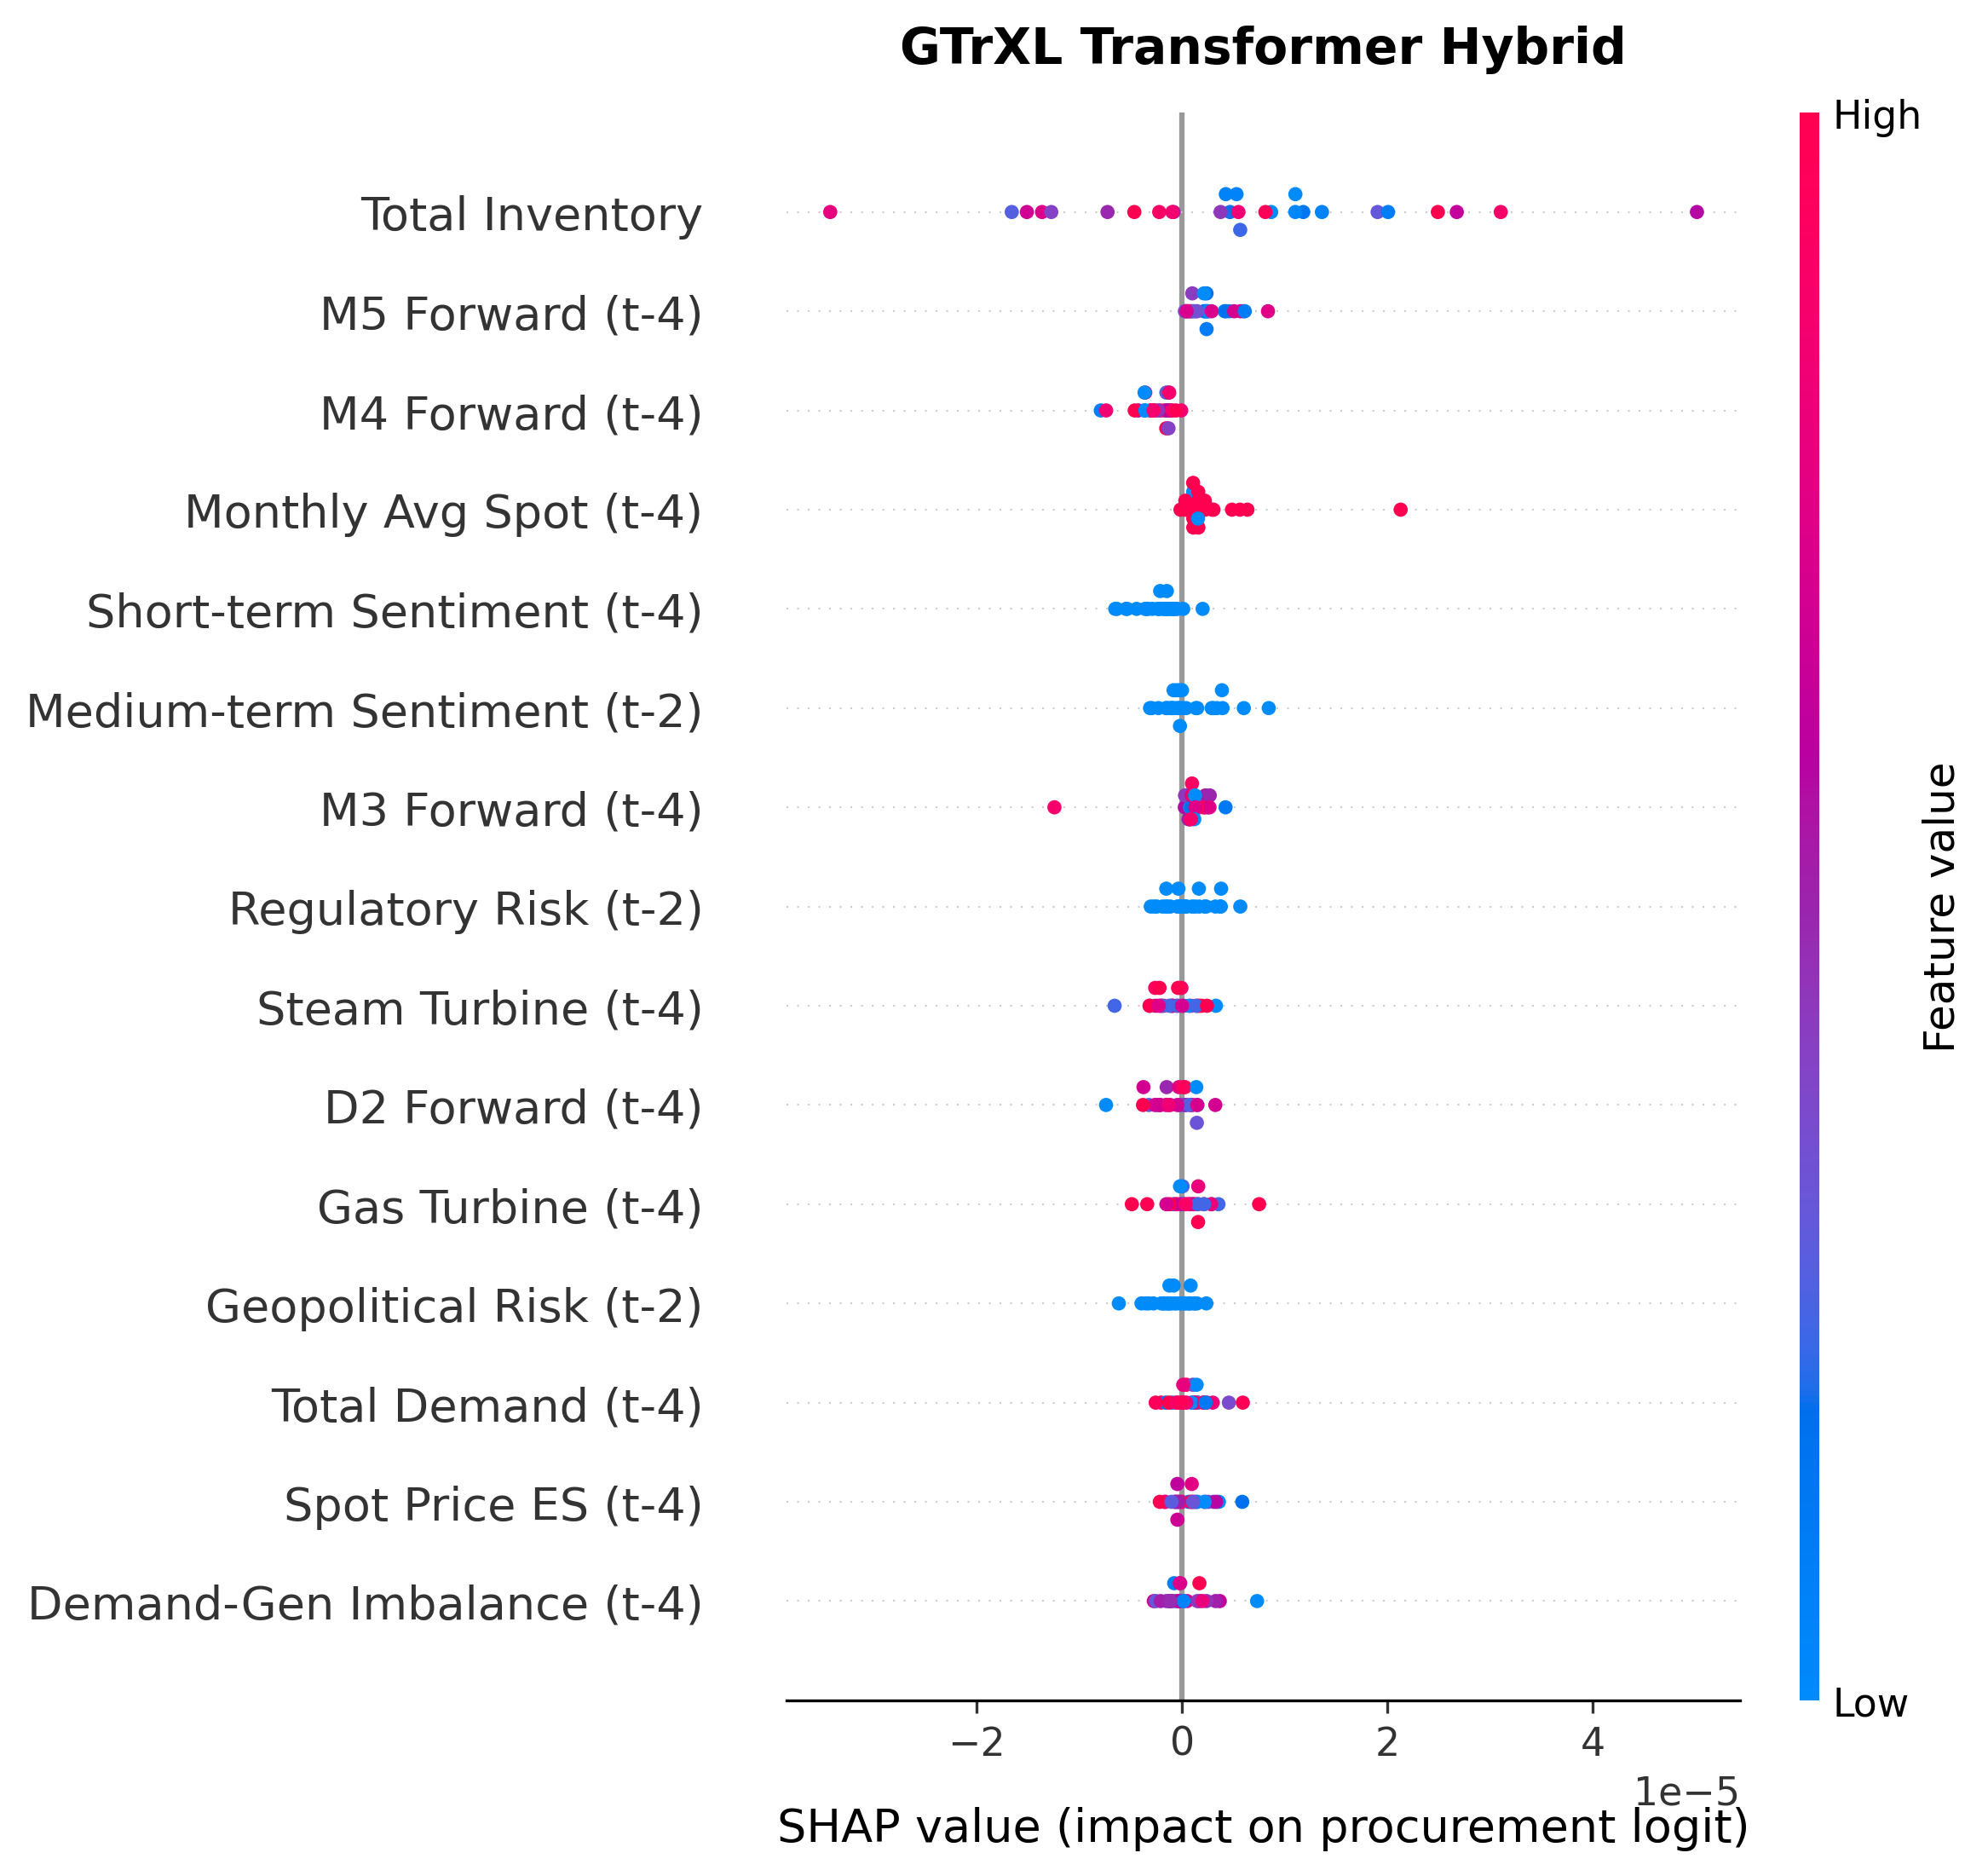
\includegraphics[width=\textwidth]{fig11_shap_transformer_hibrido.png}
        \caption{GTrXL Transformer Hybrid}
        \label{subfig:shap_gtrxl_hybrid}
    \end{subfigure}
    \hfill
    \begin{subfigure}[b]{0.48\textwidth}
        \centering
        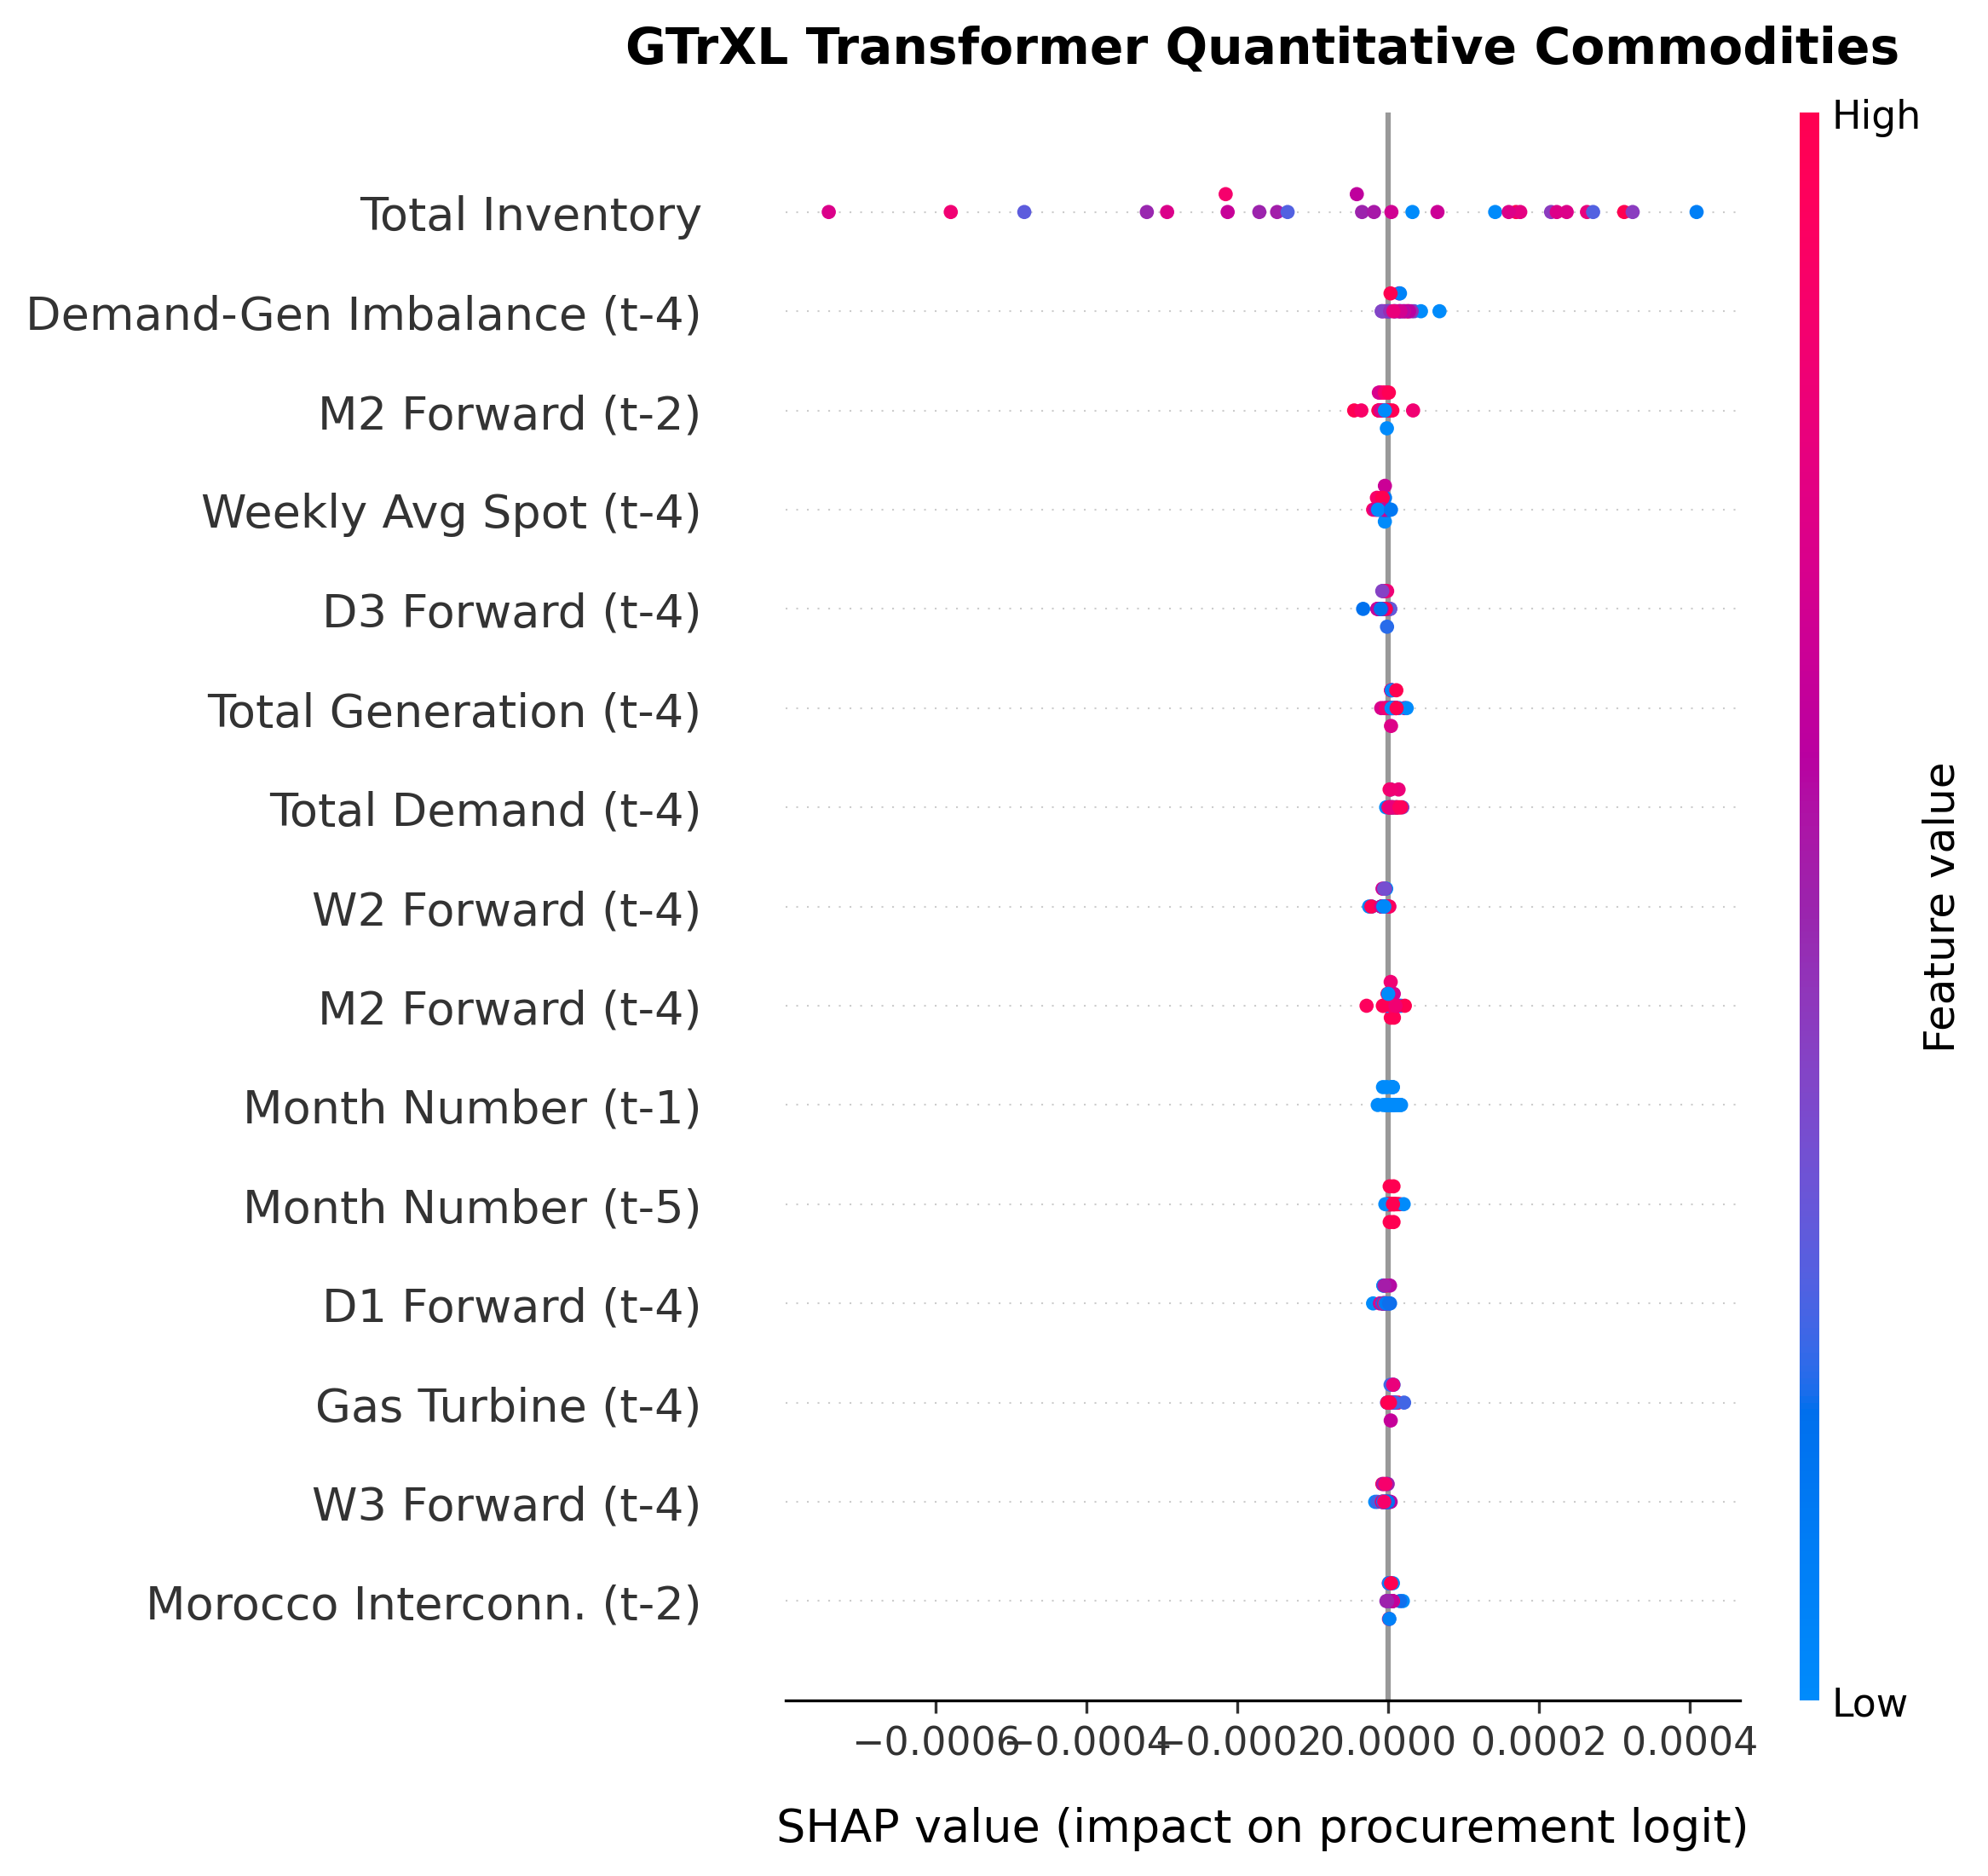
\includegraphics[width=\textwidth]{fig11_shap_transformer_fisico.png}
        \caption{GTrXL Transformer Quantitative Commodities}
        \label{subfig:shap_gtrxl_physical}
    \end{subfigure}
    \vskip\baselineskip
    \begin{subfigure}[b]{0.48\textwidth}
        \centering
        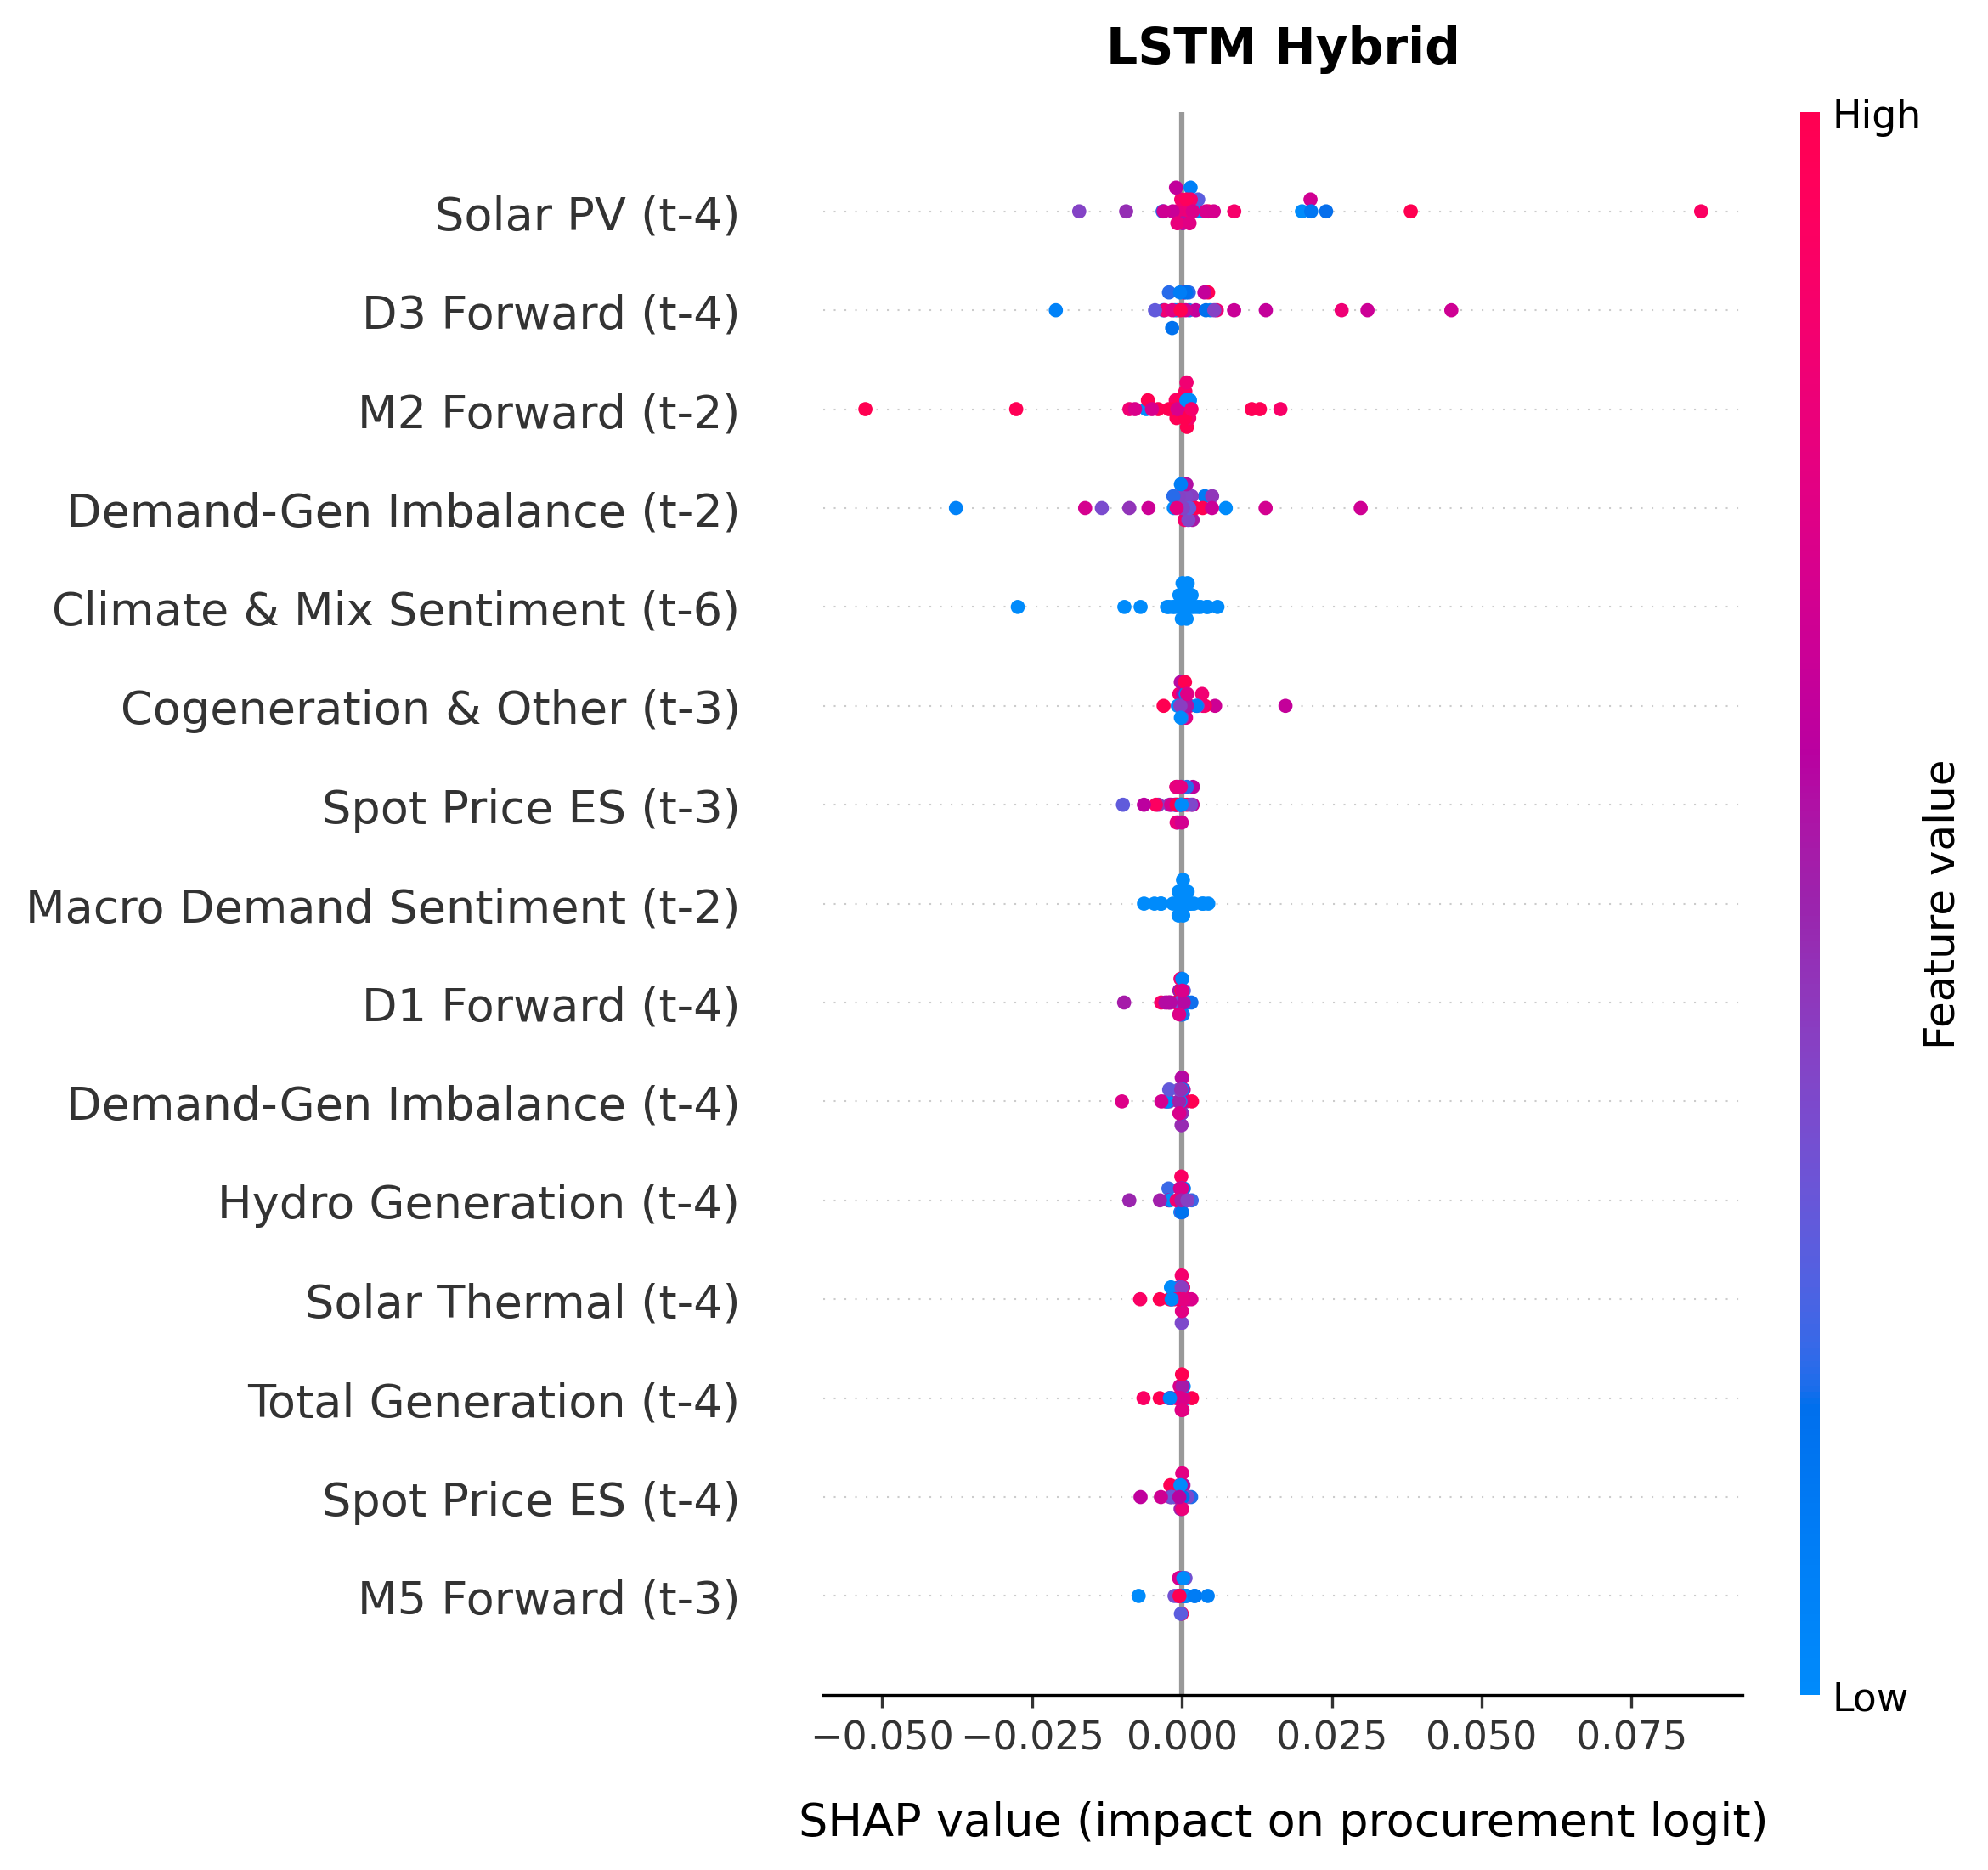
\includegraphics[width=\textwidth]{fig11_shap_lstm_hibrido.png}
        \caption{LSTM Hybrid}
        \label{subfig:shap_lstm_hybrid}
    \end{subfigure}
    \hfill
    \begin{subfigure}[b]{0.48\textwidth}
        \centering
        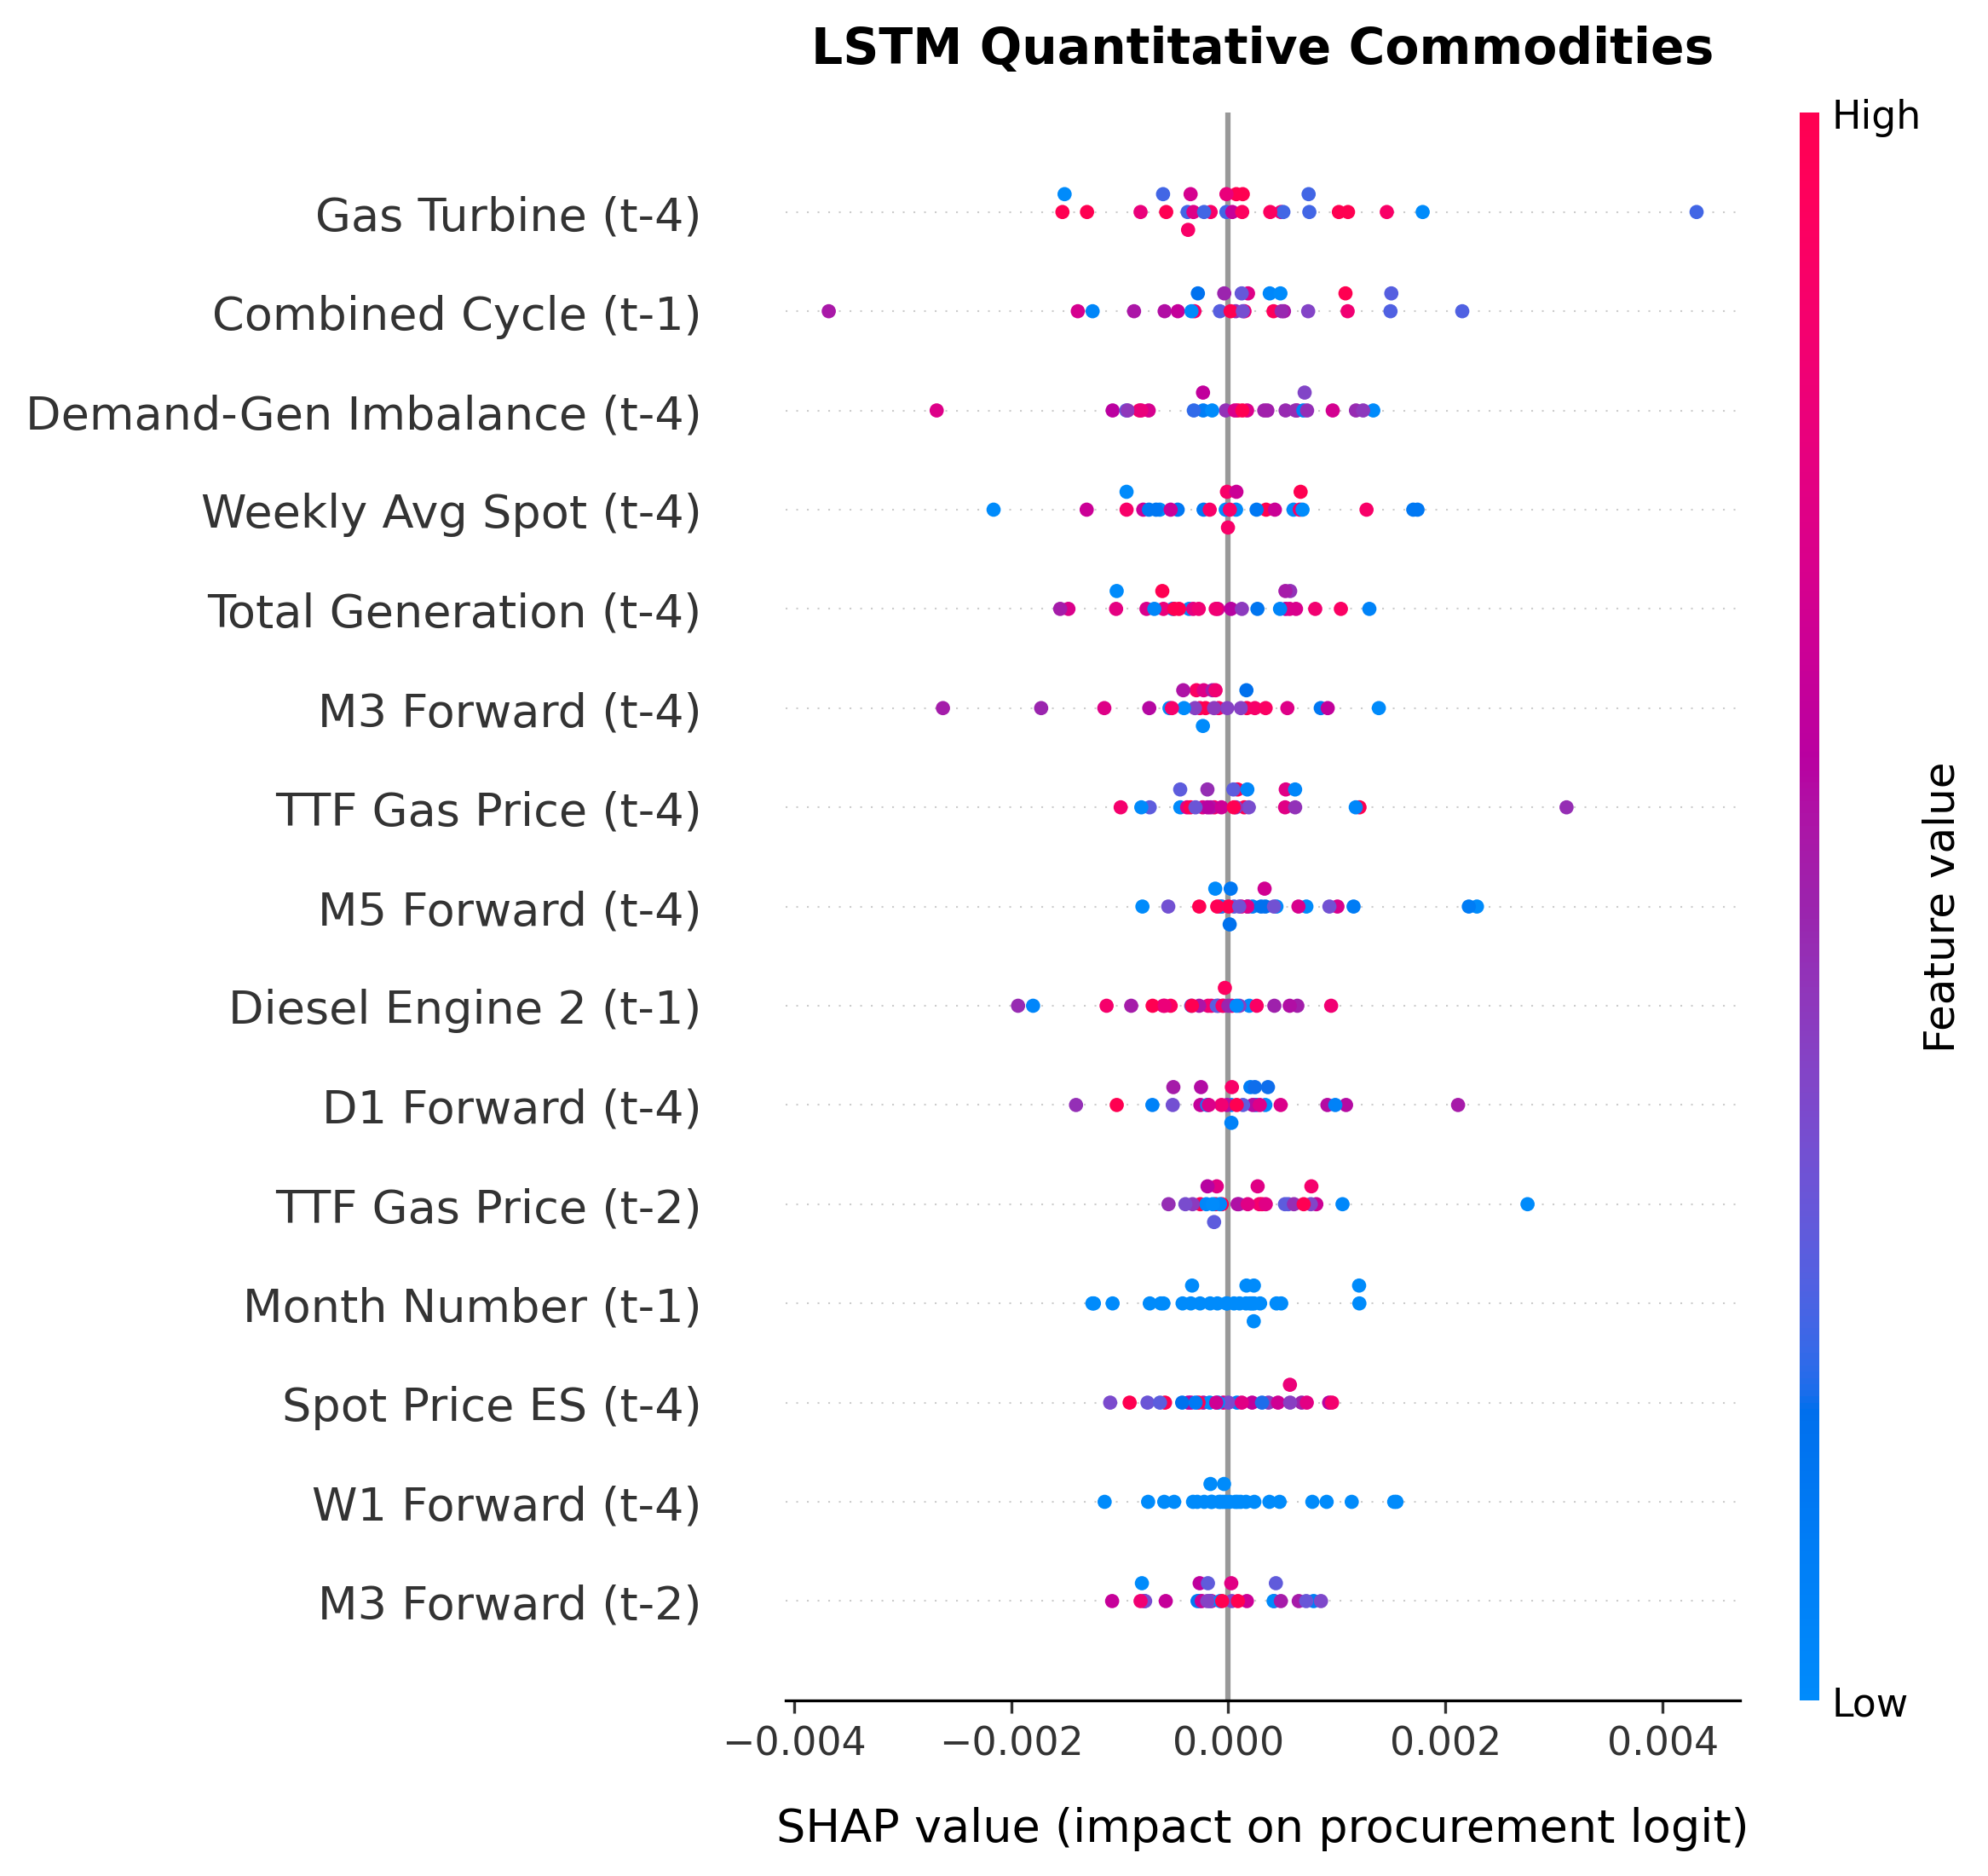
\includegraphics[width=\textwidth]{fig11_shap_lstm_fisico.png}
        \caption{LSTM Quantitative Commodities}
        \label{subfig:shap_lstm_physical}
    \end{subfigure}
    \caption{SHAP feature attribution summary across 2026 evaluation observations for Phase~4 models. Points represent daily observations colored by feature value (red: high, blue: low); horizontal dispersion reflects directional impact on policy procurement logits.}
    \label{fig:shap_comparison}
\end{figure*}

The attribution profiles in \cref{fig:shap_comparison} reveal distinct structural patterns across the evaluated configurations. In the GTrXL Hybrid model (\cref{subfig:shap_gtrxl_hybrid}), aggregated forward commitment inventory features yield the largest mean absolute SHAP magnitude among evaluated predictors (mean absolute SHAP $= 1.33 \times 10^{-5}$), showing that existing forward commitments strongly govern policy decisions. Furthermore, text-derived sentiment dimensions rank within the top 15 most influential predictors in the hybrid architectures. While the full observation vector comprises $\text{dim}(\mathbf{o}_t) = 715$ dimensions, the SHAP gradient explainer is computed over the 318 active input dimensions that exhibit non-zero gradient variance: 31 dynamic market features across $L=7$ historical lookback lags ($31 \times 7 = 217$ inputs) plus the first 101 forward inventory delivery offsets ($h \in \{1, \dots, 101\}$ days). As an empirical finding, the trained policies never selected long-horizon forward contracts ($M_4$--$M_6$), leaving delivery offsets $h > 101$ days at zero allocation ($m_t(h)=0$) with constant sentinel values $-10.0$ and identically zero gradients. Specifically, short-term sentiment (\texttt{Short-term Sentiment}, rank 6), medium-term sentiment (\texttt{Medium-term Sentiment}, rank 7), regulatory intervention risk (\texttt{Regulatory Intervention Risk}, rank 9), and geopolitical risk (\texttt{Geopolitical Risk}, rank 13) exhibit high attribution magnitude, with heightened geopolitical risk scores systematically associated with elevated logits for short-horizon forward contracts ($D_2/D_3$). In contrast, for the LSTM Hybrid model (\cref{subfig:shap_lstm_hybrid}), physical grid coupling variables---most notably solar PV generation (\texttt{Solar PV}) and the generation-demand imbalance (\texttt{Generation-Demand Imbalance})---dominate the highest attribution ranks alongside forward contract quotes ($D_3$, $M_2$), while climate and generation mix sentiment (\texttt{Climate \& Mix Sentiment}, rank 6) and macroeconomic demand sentiment (\texttt{Macroeconomic Demand}, rank 9) receive non-negligible attribution.

These attribution results describe empirical associations between input features and policy outputs within the evaluated sample conditioned on the lookback window and $h_0 = \mathbf{0}$. We emphasize that SHAP attributions reflect internal directional associations between input gradients and policy logits in the fitted Phase~4 models (whose architecture hyperparameters were tuned across the full horizon). Consequently, these feature attributions describe the internal decision logic of the post-selection network rather than providing an independent validation of semantic construct validity, proving a structural causal relationship between news sentiment and forward price dynamics, or demonstrating that the agent explicitly forecasts market price collapses. The near-zero attribution assigned to distant collinear indicators is consistent with effective representation filtering on local observation gradients, focusing policy sensitivity on high-relevance physical balances and regulatory sentiment while attenuating redundant market signals within the evaluated state space.

% ── Section 6: Discussion ───────────────────────────────────────────────────
\section{Discussion}
\label{sec:discussion}

The results highlight the varying adaptive capacities of reinforcement learning procurement policies operating under non-stationary market regimes. Across the evaluated configurations, the MLP showed the least stable performance, whereas the LSTM provided more conservative behaviour. The GTrXL configurations achieved higher mean savings in the Walk-Forward evaluation, particularly when combined with the NLP features.

The Multi-Layer Perceptron (MLP) demonstrated unstable performance during the static 2025 evaluation, suggesting that its lack of temporal memory restricts adaptation to distributional shifts. Conversely, the RecurrentPPO (LSTM) agent converged to a single-contract policy under static evaluation, prioritising the D2 contract. Under the Walk-Forward evaluation without NLP data, the LSTM Quantitative Commodities Baseline model yielded mean losses ($-2.00\%$), indicating that sequence memory alone was insufficient to maintain positive savings given only quantitative features.

\subsection{Characterisation of Low-Entropy Policy Convergence}

In the evaluated static runs, the recurrent policy converged to a low-entropy behaviour dominated by D2 selections. This concentration reduced exposure to longer-horizon contracts but also limited the range of procurement actions available to the policy. This behaviour is compatible with the combined effect of delayed reward realization at delivery, non-overlapping contract penalties, and exponential temporal discounting ($\gamma=0.99$), although our experiments do not isolate the individual contribution of each mechanism.

The Walk-Forward findings indicate that this low-entropy convergence is mitigated when the state representation includes multimodal information under continuous retraining. The Hybrid representation (\texttt{Dataset\_M8\_Physical\_NLP}), combining physical fundamentals with targeted macroeconomic sentiment, yields a more balanced action profile (D2: 51.6\%, D1: 17.9\%, SPOT: 16.6\%, D3: 13.9\%) while maintaining positive simulated savings during the 2026 shock (+6.32\%).

A central theoretical consideration is the functional role of zero-shot LLM news sentiment as an alternative representation. Under stationary conditions, quantitative commodity prices and historical generation curves provide direct econometric signals for forward pricing. However, when wholesale market dislocations occur---such as the renewable price cannibalisation observed in Iberia in 2026---historical empirical correlations between international fossil fuel prices (Brent, TTF, EU ETS) and local electricity clearing prices may decouple. The sentiment variables offered an alternative representation of regulatory, geopolitical, and generation-related information. Their inclusion coincided with positive savings (+6.32\%) during the 2026 evaluation period, although the present experiments do not establish whether this improvement resulted primarily from semantic narrative signals, feature dimensionality, noise filtering, or interactions with the policy architecture. Establishing a formal causal regime-filtering mechanism would require an independently held-out multi-year period and explicit econometric time-varying-parameter tests.

This progression is reflected in the Phase 4 results. The sentiment variables added information that was not strongly collinear with several physical features in the descriptive PCA and were associated with higher procurement savings in the evaluated configurations. Augmenting the state representation with lagged news-derived sentiment on LNG availability, regulatory developments, and geopolitical risk yielded $+9.36\%$ mean savings ($\sigma=1.37\%$) for the LSTM Hybrid model, compared to the quantitative commodity baseline ($-2.00\%$, $\sigma=1.56\%$). This difference is consistent with an incremental contribution from qualitative news sentiment relative to numerical commodity futures during the evaluated shift.

In the evaluated setting, the GTrXL configuration achieved higher mean savings than the LSTM configuration. The Transformer Quantitative Commodities model reached $+9.97\%$ ($\sigma=1.32\%$). The Hybrid Transformer model yielded $+10.85\%$ mean savings, accompanied by a reduction in across-seed standard deviation to $\sigma=0.63\%$. Across-seed standard deviation ($\sigma_{\text{seeds}}$) quantifies algorithmic optimization stability under stochastic neural initialization rather than downside financial risk (e.g., CVaR or maximum drawdown). Future industrial extensions should incorporate explicit risk-averse utility functions (such as distributional RL or spectral risk penalties) to directly penalize tail loss events during market spikes.

\subsection{Economic Evaluation: Dynamic Multi-Horizon DRL vs.\ Partial Hedging and Static Heuristics}
\label{subsec:economic_evaluation}

An essential operational and scientific question is why an industrial consumer or energy procurement manager should deploy a complex reinforcement learning policy rather than executing a simple passive procurement heuristic---such as systematic $D_2$ purchasing or a static partial hedging rule ($\alpha \cdot D_2 + (1-\alpha) \cdot \text{SPOT}$). Across the annual Walk-Forward evaluations (Table~\ref{tab:annual_rl_vs_d2}) and the 2026 isolated shock (Table~\ref{tab:blind_2026_comparison}), the mechanical $100\%$ $D_2$ heuristic achieved higher nominal savings ($+11.18\%$ to $+15.67\%$) than the evaluated RecurrentPPO policy ($+5.45\%$ to $+6.74\%$). During the isolated January--May 2026 evaluation, M8-W1 achieved $6.32\%$ simulated savings, compared with $11.18\%$ for the passive $D_2$ rule and $5.59\%$ for a $50\% D_2 / 50\% \text{SPOT}$ hedge. The policy had lower downside semi-deviation than $D_2$ ($9.15$ versus $13.68$~\texteuro/MWh) and a lower maximum drawdown ($186.45$ versus $225.45$~\texteuro/MWh), but its paired savings differences against $D_2$ and the balanced hedge had moving-block bootstrap confidence intervals that included zero. The results therefore suggest a different savings--risk profile in this episode, rather than statistically established savings superiority. The 2026 window represents a single market-dislocation episode and cannot establish general regime robustness.

This empirical divergence raises fundamental economic considerations regarding the true objective of procurement policies in volatile energy markets. We delineate four critical operational and risk-management considerations regarding dynamic reinforcement learning relative to static heuristics:

\subsubsection{Historical Sample Bias and Forward--Spot Differentials}

The high nominal savings of the mechanical $D_2$ rule in the evaluated sample are consistent with a horizon-dependent forward--spot differential, but the present data do not identify its cause. Risk premia, market-maker quotes, liquidity conditions, delivery-horizon effects, and sample-specific market dynamics may all contribute~\cite{huisman2012electricity, woo2001cross}. In the absence of direct participant, bid--ask, order-book, and renewable-forecast-error data, we do not attribute the observed differential specifically to renewable forecast errors or to a causal market mechanism.

Relying on the persistence of a single market anomaly represents an unhedged speculative bet on market microstructure stationarity. When market rules change, when forecasting tools evolve, or when liquidity migrates, historical forward discounts can invert rapidly. In our empirical sample, identical mechanical purchasing on $D_1$ yielded negative savings ($-1.30\%$), $D_3$ suffered high downside volatility ($\sigma_- = 18.63$~\texteuro/MWh) and substantial drawdown ($548.95$~\texteuro/MWh), and longer-term monthly contracts collapsed to severe losses ($-20.72\%$ for $M_3$, $-31.61\%$ for $M_4$, and $-49.95\%$ in 2023). A static heuristic possesses no mechanism to detect when a discount has evaporated; it continues executing blindly until major drawdown occurs.

\subsubsection{Comparison against the Partial Hedging Continuum \texorpdfstring{($\alpha \cdot D_2 + (1-\alpha) \cdot \text{SPOT}$)}{(D2--SPOT Combinations)}}

Industrial risk managers rarely execute $100\%$ unhedged SPOT or $100\%$ single-instrument forwards; instead, corporate hedging mandates typically prescribe linear partial hedging mixtures $\alpha \in [0, 1]$. As formalized in Panel~A of Table~\ref{tab:blind_2026_comparison}, a static partial hedge linearly interpolates both return and downside risk ($g_t(\alpha) = \alpha \cdot g_t(D_2)$). A balanced $50\%\, D_2 + 50\%\, \text{SPOT}$ policy achieves $+5.59\%$ savings with a maximum drawdown of $112.73$~\texteuro/MWh.

The dynamic DRL agent (M8-W1) achieves a point estimate of $+6.32\%$ savings, compared with $+5.59\%$ for the balanced $50\%$ partial hedge ($+0.73$~pp difference, $d_t = +0.32$~\texteuro/MWh). However, because the paired 95\% moving-block bootstrap confidence interval spans $[-3.10, +5.91]$~pp, this difference does not establish statistically significant savings superiority over the balanced hedge. Instead, the dynamic policy demonstrates an alternative savings--risk profile: rather than maintaining an inflexible static ratio, the DRL agent dynamically modulates its allocation conditional on daily market fundamentals and macroeconomic news sentiment: holding SPOT unhedged when pool prices are projected to collapse (16.6\% of sessions), and dynamically selecting between $D_1$ (17.9\%), $D_2$ (51.6\%), and $D_3$ (13.9\%) depending on where the forward risk premium is concentrated. In the Phase~4 capacity evaluation, the GTrXL Transformer agent achieved $+10.85\%$ savings, matching the nominal return level of mechanical $D_2$ ($+11.18\%$) while maintaining a diversified multi-horizon execution profile.

\subsubsection{Action Diversification across Horizons vs.\ Static Concentration}

A notable operational consideration regarding the mechanical $100\%$ $D_2$ strategy is single-instrument market concentration. On organized derivative exchanges such as OMIP, short-dated daily forward contracts ($D_1, D_2, D_3$) exhibit finite order-book liquidity and depth. For a large industrial enterprise or aggregator consuming, for example, 50 to 200~MW of continuous baseload ($1{,}200$ to $4{,}800$~MWh/day), attempting to purchase $100\%$ of required delivery volume exclusively on the $D_2$ order book every morning would concentrate execution exposure in a single instrument.

In contrast, the dynamic DRL policy demonstrates simulated action diversification across horizons: order flow is distributed across $D_1$ (17.9\%), $D_2$ (51.6\%), $D_3$ (13.9\%), and SPOT daily clearing auctions (16.6\%). We caution that our simulation environment does not model order-book depth, bid--ask spreads, or non-linear market impact; therefore, this multi-horizon distribution demonstrates policy flexibility and diversification within the simulation, rather than empirical proof of reduced market impact in physical execution.

\subsubsection{Regime-Adaptive Risk Management vs.\ Static Fragility}

Ultimately, the primary scientific and economic finding of the proposed framework is not claiming unconditional return dominance over an isolated historical anomaly, but evaluating an \textbf{adaptive multi-horizon risk mitigator}. In energy procurement, downside risk---quantified by Downside Semi-deviation ($\sigma_-$), Conditional Value at Risk ($\text{CVaR}_{0.95}$), and Maximum Drawdown---is often more critical for corporate solvency than nominal return maximization.

During the 2026 wholesale price dislocation, the dynamic M8-W1 policy reduced downside semi-deviation from $13.68$ to $9.15$~\texteuro/MWh (for $D_2$, a $33.1\%$ volatility reduction) and lowered maximum drawdown from $225.45$ to $186.45$~\texteuro/MWh. Compared to alternative forward contracts such as $D_3$ (Max DD $= 548.95$~\texteuro/MWh), the RL policy cut maximum drawdown by nearly two-thirds in this sample. By combining physical generation state variables with forward-looking macroeconomic news sentiment, the DRL agent actively navigates non-stationary market regimes, offering corporate buyers an alternative multi-horizon hedging profile that curtails extreme tail losses when historical market correlations breakdown.
\subsection{Transaction Cost Sensitivity Analysis}
\label{subsec:trans_costs}

The primary backtest evaluations assume frictionless forward execution ($C_0 = 0.00$~\texteuro/MWh) to isolate the theoretical settlement-implied procurement efficiency of the learned policy. In industrial wholesale electricity trading, continuous hedging via broker-intermediated OTC contracts or organized derivatives exchanges (such as OMIP and OMIClear) incurs clearing fees, exchange registration tariffs, and bid--ask half-spreads. While general power market literature reports that execution tariffs and effective spreads typically range between $0.05$ and $0.25$~\texteuro/MWh~\cite{weron2014electricity}, exact costs depend on consumer volume, exchange membership, and broker bilateral arrangements.

To assess policy sensitivity under market frictions, we conducted an exploratory sensitivity analysis across three illustrative linear transaction-cost stress scenarios applied to all executed forward contracts: a frictionless baseline ($C_0 = 0.00$~\texteuro/MWh), a moderate illustrative friction tier ($C_1 = 0.10$~\texteuro/MWh), and an adverse friction stress scenario ($C_2 = 0.25$~\texteuro/MWh). We emphasize that these are synthetic linear sensitivity tiers rather than costs observed directly from OMIP order books.

The arithmetic of the cost impact is formally derived from the empirical delivery settlement log. Percentage procurement savings relative to spot clearing are defined as $\text{Savings} = (\bar{P}_{\text{SPOT}} - \bar{P}_{\text{effective}}) / \bar{P}_{\text{SPOT}}$. When an execution fee $C$ (\texteuro/MWh) is incurred on forward contracts, effective procurement unit expenditure rises by $f_{\text{fwd}} \cdot C$, where $f_{\text{fwd}}$ represents the empirical fraction of delivered MWh settled under locked forward positions (with the residual $1 - f_{\text{fwd}}$ defaulting to unhedged spot clearing without forward execution fees). From the multi-year Walk-Forward decision and delivery log across matched evaluation cohorts, forward commitments covered exactly $f_{\text{fwd}} = 85.8\%$ of delivery days ($321$ of 374 evaluated days: $53.5\%$ under $D_2$, $17.6\%$ under $D_1$, and $14.7\%$ under $D_3$), while unhedged spot clearing settled the remaining $14.2\%$ ($53$ days), against an empirical mean spot price of $\bar{P}_{\text{SPOT}} = 65.76$~\texteuro/MWh across those 374 evaluated days. In the early-2026 Walk-Forward test blocks (44 evaluated days), forward delivery commitments accounted for $f_{\text{fwd}} = 75.0\%$ ($33$ of 44 days under $D_2$) and spot clearing settled $25.0\%$ ($11$ days), against a mean spot price of $\bar{P}_{\text{SPOT}} = 36.41$~\texteuro/MWh across those 44 evaluated days. The resulting percentage reduction in savings is $\Delta \text{Savings} = (f_{\text{fwd}} \cdot C) / \bar{P}_{\text{SPOT}}$:
\begin{itemize}
    \item \textbf{Full Walk-Forward Horizon} (374 days, $\bar{P}_{\text{SPOT}} = 65.76$ \texteuro/MWh, $f_{\text{fwd}} = 85.8\%$): For $C_1 = 0.10$ \texteuro/MWh, the expected friction is $0.0858$ \texteuro/MWh, reducing net savings by $0.0858 / 65.76 \approx 0.13$~pp ($+6.04\% \to +5.91\%$). For $C_2 = 0.25$ \texteuro/MWh, the friction is $0.2146$ \texteuro/MWh, reducing net savings by $0.2146 / 65.76 \approx 0.33$~pp ($+6.04\% \to +5.71\%$).
    \item \textbf{2026 Walk-Forward Test Blocks} (44 days, $\bar{P}_{\text{SPOT}} = 36.41$ \texteuro/MWh, $f_{\text{fwd}} = 75.0\%$): For $C_1 = 0.10$ \texteuro/MWh, the expected friction is $0.0750$ \texteuro/MWh, reducing net savings by $0.0750 / 36.41 \approx 0.21$~pp ($+6.32\% \to +6.11\%$). For $C_2 = 0.25$ \texteuro/MWh, the friction is $0.1875$ \texteuro/MWh, reducing net savings by $0.1875 / 36.41 \approx 0.51$~pp ($+6.32\% \to +5.80\%$).
\end{itemize}

\begin{table*}[htbp]
\centering
\footnotesize
\setlength{\tabcolsep}{3.5pt}
\caption{Sensitivity of Walk-Forward procurement savings to illustrative linear forward execution transaction costs ($C$, \texteuro/MWh) based on empirical delivery settlement logs across matched evaluation horizons.}
\label{tab:trans_cost_sensitivity}
\begin{tabularx}{\linewidth}{@{}l >{\raggedright\arraybackslash}X ccc@{}}
\toprule
\textbf{Cost Tier} & \textbf{Illustrative Cost Description} & \textbf{Full Horizon (374 d)} & \textbf{2026 WF (44 d)} & \textbf{Net} \\
\textbf{($C$, \texteuro/MWh)} & & \textbf{Savings (\%)} & \textbf{Savings (\%)} & \textbf{Viability} \\
\midrule
$C_0 = 0.00$ & Frictionless baseline & $+6.04\%$ & $+6.32\%$ & Baseline \\
$C_1 = 0.10$ & Moderate illustrative friction & $+5.91\%$ & $+6.11\%$ & Positive \\
$C_2 = 0.25$ & Adverse illustrative stress tier & $+5.71\%$ & $+5.80\%$ & Positive \\
\bottomrule
\end{tabularx}
\end{table*}

As shown in Table~\ref{tab:trans_cost_sensitivity}, simulated net procurement savings remain positive across all tested linear cost scenarios. Under the adverse friction assumption ($C_2 = 0.25$~\texteuro/MWh), the Walk-Forward M8 policy retains $+5.71\%$ net savings across the full evaluation horizon (374 days) and $+5.80\%$ during the 2026 Walk-Forward test blocks (44 days). Under the illustrative linear-cost assumptions examined, simulated savings remain positive. These calculations are a sensitivity analysis rather than an estimate of realized execution costs, because the environment does not model order-book depth, bid--ask spreads, or non-linear market impact.

\subsection{Limitations and Threats to Validity}

Despite the empirical performance, several limitations must be acknowledged:

First, holding total monthly PPO training interactions fixed at $K = 15{,}000$ steps across all sliding window lengths reflects an operational computational budget constraint. A short update window ($W=1$ month, $N_W \approx 20$ sessions) receives $\approx 750$ gradient interaction steps per historical observation, a quarterly window ($W=3$ months) receives $\approx 250$ steps/obs, a semi-annual window ($W=6$ months) receives $\approx 125$ steps/obs, whereas an annual window ($W=12$ months, $N_W \approx 240$ sessions) receives $\approx 62.5$ steps per observation. While fixing $K$ represents an operationally viable deployment protocol with deterministic monthly retraining latency, an alternative experimental design would scale $K$ proportionally with window size ($K(W) = 750 \times N_W$, scaling up to $K \approx 180{,}000$ for $W=12$) to hold optimization intensity per observation constant. Future work should evaluate this proportional scaling ablation to formally decouple sample recency from per-sample gradient budget.

Second, the choice of discount factor $\gamma = 0.99$ introduces temporal discounting of distant cash flows ($\gamma^{30} \approx 0.74, \gamma^{90} \approx 0.40, \gamma^{180} \approx 0.16$). In conjunction with single-instrument full-volume baseload commitments and non-overlapping forward masking, geometric discounting may comparatively reduce the learning gradient signal associated with distant delivery horizons ($M_1$--$M_6$), guiding policy optimization toward contracts with immediate delivery proximity ($D_1$--$D_3$). The observed policy concentration on short-horizon products is therefore jointly shaped by the empirical forward--spot risk premia and temporal MDP mechanics.

Third, regarding temporal integrity, the LLM sentiment extraction was executed locally using the Llama-3 model with zero internet access during inference, ensuring data privacy, absence of external API drift, and strict computational repeatability under deterministic decoding. While deterministic decoding under the reported software configuration ($T=0.0$, top-$p=1.0$, strict JSON schema) enforces syntactic and computational repeatability, future work could further substantiate semantic construct validity by benchmarking against an independent human-annotated corpus. Measuring inter-annotator agreement (using weighted Cohen's $\kappa$ for ordinal categories and Intraclass Correlation Coefficients or Spearman rank correlations for continuous indices) across domain-expert annotations would provide additional external validation for specialized energy-market sentiment models. Furthermore, to conclusively demonstrate that the performance gains of the Hybrid representation stem from genuine semantic directionality rather than implicit dimensional regularisation (i.e., expanding the feature vector from 35 to 45 dimensions), a future ablation could substitute the 10 NLP sentiment signals ($\phi_1, \dots, \phi_{10}$) with matched Gaussian noise $\boldsymbol{\epsilon} \sim \mathcal{N}(\boldsymbol{\mu}_{\text{NLP}}, \boldsymbol{\Sigma}_{\text{NLP}})$. Nevertheless, the SHAP feature attribution analysis in Section~\ref{subsec:res_shap} confirms that the policy logits systematically attend to domain-coherent news dimensions (such as regulatory risk and generation mix), corroborating the semantic grounding of the extracted features.

Fourth, Phases 1 and 2 report single-seed point estimates across the 8-dataset ablation space. While computationally necessary to explore the broad factorial design space before committing to the intensive multi-seed retraining protocol, the descriptive interaction observed in Phase~1 remains preliminary until multi-seed replications and dimension-matched noise controls across all factorial cells are executed. Multi-seed validation was rigorously performed for all continuous Walk-Forward and capacity evaluations in Phases 3 and 4 across 5 independent seeds.

Fifth, in alignment with standard machine-learning validation protocols, the 2025 horizon served as the preliminary validation partition to discard unviable heuristics and prune unpromising feature representations. Consequently, the multi-year continuous Walk-Forward evaluation preserves the 2026 horizon (January--May 2026, comprising 102 official OMIP trading sessions [decision epochs] and 46 non-trading dates [3 TARGET closures and 43 weekend days] within 148 calendar delivery days) as a strictly forward-looking, sequentially out-of-sample benchmark (with each monthly decision conditioned only on information available prior to that evaluation block) to test resilience under the wholesale price dislocation.

Sixth, the evaluation horizon for 2026 covers January--May 2026 (102 official OMIP trading sessions [decision epochs] and 46 non-trading dates [3 TARGET closures and 43 weekend days] across 148 calendar delivery days), corresponding to the data available at the time of study. Whether the performance advantages of \texttt{Dataset\_\allowbreak M8\_\allowbreak Physical\_\allowbreak NLP} over \texttt{Dataset\_\allowbreak NLP\_\allowbreak Subgroups} persist through subsequent seasonal cycles remains to be verified as additional market data become available.

Seventh, hyperparameter optimisation (Phase 4) was performed using a fixed seed ($s=42$) on the Hybrid representation and transferred to the Quantitative Baseline to isolate architectural capacity. While validated subsequently across multiple seeds, the HPO search itself reflects trajectory dynamics of that initialisation and naturally optimizes hyperparameters on the Hybrid feature space. Furthermore, the Phase 4 result is an exploratory post-selection capacity analysis over the 2026 horizon, not an unbiased out-of-sample evaluation. Finally, formal corrections for multiple comparisons (Bonferroni) were applied to the joint family of KS-tests but not to the multi-dataset ablation study in Phase 1, introducing the potential for family-wise error.

Eighth, while Section~\ref{subsec:trans_costs} establishes that net savings remain positive under proportional linear transaction fees up to $0.25$~\texteuro/MWh, the simulated environment does not model non-linear order book depth, market impact, or slippage during thin-volume trading sessions. Although all performance metrics are normalized to a 1~MW continuous baseload capacity ($E_{\text{load}, d} = 24$~MWh/day) and scale linearly, deploying large physical volumes (such as a 200~MW enterprise demand) on short-dated contracts ($D_1$--$D_3$) would be constrained by daily exchange liquidity and order-book depth. Future operational deployments should integrate execution cost models with live order-book depth to evaluate net procurement savings under strict market microstructure constraints.



% ── Section 7: Conclusion ───────────────────────────────────────────────────
\section{Conclusion}
\label{sec:conclusion}

This study evaluated a sequential framework for consumer-side electricity procurement across spot and OMIP forward contracts, combining physical system variables, quoted derivative prices, and macroeconomic news sentiment extracted with a large language model. The empirical analysis provides three primary findings.

First, econometric tests indicate that news-derived sentiment contains conditional predictive information for forward basis dynamics beyond physical variables and quantitative commodity indicators. In the 2025 single-seed ablation, adding sentiment to the physical baseline yielded an increase in simulated savings (from $7.48\%$ to $11.66\%$), whereas combining sentiment with commodity features showed a negative descriptive interaction ($-2.59$~pp), indicating that information from these feature blocks is not simply additive.

Second, during the evaluated 2026 price-dislocation window, the re-trained M8-W1 policy achieved positive simulated savings ($+6.32\%$) and lower downside semi-deviation ($9.15$ vs $13.68$~\texteuro/MWh) and lower maximum drawdown ($186.45$ vs $225.45$ \texteuro/MWh) than passive $D_2$, while $D_2$ achieved greater nominal savings ($+11.18\%$). Pairwise confidence intervals do not establish that M8-W1 delivers higher savings than either $D_2$ or a balanced 50/50 partial hedge ($+5.59\%$, 95\% CI: $[-3.10, +5.91]$~pp). The evidence is thus consistent with a potential risk--return trade-off from dynamic multi-horizon allocation under the conditions evaluated, not with unconditional economic superiority or a general anti-fragile property.

Finally, frequent rolling retraining was associated with sustained positive simulated performance under market transitions: updating policy networks on recent historical windows maintained positive savings when historical correlations between power prices and international fossil commodities decoupled. Further work should replicate the factorial ablation across multiple random seeds, incorporate dimension-matched noise controls, validate the sentiment signals against domain-expert annotations, and evaluate additional out-of-sample market regimes and non-linear order-book execution frictions.


%% ── Declarations / Back Matter ──────────────────────────────────────────────
\section*{CRediT authorship contribution statement}
\textbf{Manel Mart{\'i}nez-Retamal:} Conceptualization, Methodology, Software, Formal analysis, Investigation, Data curation, Writing -- Original Draft, Visualization.
\textbf{David Gualda:} Conceptualization, Methodology, Software, Validation, Supervision, Writing -- Review \& Editing.
\textbf{Reinier Herrera-Casanova:} Formal analysis, Validation, Writing -- Review \& Editing.
\textbf{Leonardo Pe\~na-Pupo:} Methodology, Formal analysis, Writing -- Review \& Editing.
\textbf{Carlos Santos-P{\'e}rez:} Conceptualization, Methodology, Supervision, Validation, Writing -- Review \& Editing, Funding acquisition.

\section*{Declaration of competing interest}
The authors declare that they have no known competing financial interests or personal relationships that could have appeared to influence the work reported in this paper.

\section*{Declaration of generative AI and AI-assisted technologies in the manuscript preparation process}
During the preparation of this work, the authors utilized Meta Llama-3 8B Instruct (quantized Q4\_K\_M, executed locally via Ollama v0.1.32) solely as an empirical natural language processing instrument to extract zero-shot continuous sentiment dimensions ($\phi_1, \dots, \phi_{10}$) from daily macroeconomic news as state variables in the reinforcement learning environment, as detailed in Section~\ref{subsec:nlp}. In addition, Anthropic Claude 3.5 Sonnet was used to assist in the conceptualization and layout design of the workflow schematic in \cref{fig:walk_forward_protocol}. The Graphical Abstract was developed entirely programmatically in Python using Matplotlib without text-to-image generative tools, in full compliance with Elsevier editorial policy. For manuscript preparation, Anthropic Claude 3.5 Sonnet and OpenAI ChatGPT (GPT-4o) were used solely for English language proofreading, grammar refinement, and readability improvements. After using these tools, the authors reviewed, verified, and edited all content, formulas, statistical tests, and data tables, and take full responsibility for the integrity and content of the published article.

\section*{Acknowledgements}
{\sloppy
This work was supported by the PREDFLEX-CM project (TEC-2024/ECO-287), funded by the Comunidad de Madrid through the R\&D activities programme ``Tecnolog\'ias 2024''; the UrbanFlex project (CM/DEMG/2024-030), funded by the Comunidad de Madrid through the convenio-subvenci\'on for the promotion of research and technology transfer at the Universidad de Alcal\'a; the RuralH2Verde project (SBPLY/24/180225/000198), funded by the European Union through the European Regional Development Fund (ERDF) and by the Castilla-La Mancha Agency for Research and Innovation (INNOCAM); the GEMECOP project (PID2022-139575OB-I00), funded by the Spanish Ministry of Science and Innovation; the VOLTAIRE project (CPP2023-010861), funded by the Ministry of Science and Innovation (MCIN\slash AEI\slash 10.13039\slash 501100011033) and the European Union NextGenerationEU/PRTR through the ``Proyectos de Colaboraci\'on P\'ublico Privada 2023'' programme; and the project ``Gesti\'on adaptativa de la congesti\'on en redes de distribuci\'on mediante flexibilidad distribuida y control aperi\'odico'' (PID2025-175026OB-I00), funded by the Spanish Ministry of Science, Innovation and Universities / Agencia Estatal de Investigaci\'on (MCIN\slash AEI\slash 10.13039\slash 501100011033).
\par}

\section*{Data availability}
{\sloppy
The complete codebase (Gymnasium MDP environments, PPO\slash LSTM\slash GTrXL architectures, local Ollama extraction pipeline with Llama-3 8B-Instruct Q4\_K\_M, zero-shot system prompts, JSON schema definitions, news deduplication and retrospective daily aggregation routines) and all processed factorial ablation datasets (2023--2026) are maintained in a structured repository hosted at \url{https://github.com/MannyKing55/mibel-drl-procurement}. In accordance with double-blind peer-review guidelines, an anonymous snapshot with scrubbed author and commit metadata is maintained via \url{https://anonymous.4open.science/}, and the primary repository will be made fully public under an open-source MIT licence upon publication. Proprietary raw settlement series are reconstructed through the automated data-engineering scripts provided in the repository, subject to access permissions from the corresponding market operators (OMIE, OMIP, REE).
\par}

%% ── Appendices (Algorithms) ──────────────────────────────────────────────────
\clearpage
\onecolumn
\appendix
\section{Continuous Walk-Forward Retraining Algorithm}
\label{app:walk_forward}

This appendix provides the formal algorithmic specification of the continuous Walk-Forward rolling retraining protocol described in Section~\ref{sec:methodology} and illustrated in \cref{fig:walk_forward_protocol}.

\bigskip
\begin{algorithm*}[t]
\caption{Continuous Walk-Forward Rolling Retraining Protocol}
\label{alg:walk_forward}
\footnotesize
\begin{algorithmic}[1]
\Require Multi-year market dataset $\mathcal{D}$, rolling update window $W \in \{1, 3, 6, 12\}$ months, evaluation step $h = 1$ month, PPO rollout steps $K = 15{,}000$, evaluation seeds $\mathcal{S} = \{10, 20, 30, 40, 50\}$.
\Ensure Multi-seed evaluation trajectories $\{\mathcal{H}_{\text{eval}}^{(s)}\}_{s \in \mathcal{S}}$, aggregate percentage savings $S_{\%}$, cumulative savings $S_{\text{cum}}$, downside risk $\sigma_-$, and $\text{CVaR}_{0.95}$.

\Statex
\For{\textbf{each} random evaluation seed $s \in \mathcal{S}$}
    \State Set deterministic seeds for PyTorch, NumPy, Python random, and gym environment to $s$.
    \State Initialize persistent physical/financial inventory state $\mathbf{c}_{\text{eval}} \leftarrow \mathbf{0}_{H}$, action mask $\mathbf{m}_{\text{eval}} \leftarrow \mathbf{0}_{H}$, policy network $\pi_\theta \leftarrow \text{None}$.
    \State Partition multi-year market timeline (2023--2026) into $B = 41$ consecutive monthly calendar blocks $\{M_1, M_2, \dots, M_B\}$.
    
    \Statex
    \Statex \textbf{\quad\textit{// --- Rolling Monthly Walk-Forward Retraining and Out-of-Sample Execution ---}}
    \For{\textbf{each} out-of-sample evaluation block index $b = W+1$ \textbf{to} $B$}
        \State Define rolling historical training slice: $\mathcal{D}_{\text{train}}^{(b)} \leftarrow \{M_{b-W}, \dots, M_{b-1}\}$ ($W$ preceding calendar months).
        \State Define sequentially out-of-sample evaluation slice: $\mathcal{D}_{\text{eval}}^{(b)} \leftarrow M_b$ (subsequent 1-month evaluation block).
        \State Fit causal standard scaler $\mathcal{S}_b$ strictly on $\mathcal{D}_{\text{train}}^{(b)}$ (strictly preventing look-ahead data leakage).
        \State Transform training and evaluation slices: $\widetilde{\mathcal{D}}_{\text{train}}^{(b)} \leftarrow \mathcal{S}_b(\mathcal{D}_{\text{train}}^{(b)})$, $\widetilde{\mathcal{D}}_{\text{eval}}^{(b)} \leftarrow \mathcal{S}_b(\mathcal{D}_{\text{eval}}^{(b)})$.
        \State Instantiate training simulation environment $\mathcal{E}_{\text{train}}(\widetilde{\mathcal{D}}_{\text{train}}^{(b)})$ with temporary episodic inventory reset $\mathbf{c}_{\text{train}} \leftarrow \mathbf{0}_H$.
        
        \If{$\pi_\theta$ is $\text{None}$}
            \State Initialize policy network $\pi_\theta$ with selected neural architecture weights $\theta$ (RecurrentPPO LSTM or GTrXL Transformer).
        \Else
            \State Bind policy $\pi_\theta$ to training environment $\mathcal{E}_{\text{train}}$ (\textit{warm-start continuous policy fine-tuning}).
        \EndIf
        
        \State Fine-tune policy $\pi_\theta$ for $K = 15{,}000$ environment interaction steps via PPO gradient updates over $\widetilde{\mathcal{D}}_{\text{train}}^{(b)}$.
        \State Freeze policy weights $\pi_\theta$ and fitted scaler $\mathcal{S}_b$.
        
        \Statex
        \Statex \textbf{\quad\quad\textit{// --- Out-of-Sample Sequential Trading and Settlement Valuation (Inside Block $b$) ---}}
        \State Instantiate evaluation environment $\mathcal{E}_{\text{eval}}(\widetilde{\mathcal{D}}_{\text{eval}}^{(b)})$ and inject real persistent physical inventory $\mathbf{c}_{\text{eval}}$ and active forward mask $\mathbf{m}_{\text{eval}}$.
        \State Reset $\mathcal{E}_{\text{eval}}$ with 20-day historical lookback buffer ($t_{\text{start}} = 20$), cleanly resetting latent recurrent state $h_0 \leftarrow \mathbf{0}$ (\texttt{episode\_starts = True}).
        
        \For{\textbf{each} out-of-sample delivery day $t = 21$ \textbf{to} $|\mathcal{D}_{\text{eval}}^{(b)}|$}
            \State Settle mature forward baseload commitments delivered on day $t$ from index $\mathbf{c}_{\text{eval}}(1)$.
            \If{OMIP derivatives market is open on day $t$ (active trading session)}
                \State Select deterministic forward contract action: $a_t = \arg\max_a \pi_\theta(a \mid \mathbf{o}_t, h_{t-1})$.
                \State Value the selected forward exposure at official OMIP settlement quote $P_{a_t, t}$ and update committed inventory $\mathbf{c}_{\text{eval}}^+$.
            \Else \Comment{Weekend, public holiday, or market closure}
                \State Set fallback action to \texttt{NO\_TRADE} ($a_t = \text{SPOT}$); fulfill unhedged base load at OMIE spot pool clearing price $P_{\text{SPOT}, t}$.
            \EndIf
            \State Step environment: advance delivery queue $\mathbf{c}_{\text{eval}}(\delta) \leftarrow \mathbf{c}_{\text{eval}}^+(\delta+1)$ for $\delta \in \{1, \dots, H-1\}$.
            \State Record daily effective unit procurement cost $P_{\text{eff}, t}$, spot benchmark $P_{\text{SPOT}, t}$, and action $a_t$ in trajectory $\mathcal{H}_{\text{eval}}^{(s)}$.
        \EndFor
        \State Propagate ending evaluation inventory state into next monthly block: $\mathbf{c}_{\text{eval}} \leftarrow \mathcal{E}_{\text{eval}}.\mathbf{c}$, $\mathbf{m}_{\text{eval}} \leftarrow \mathcal{E}_{\text{eval}}.\mathbf{m}$.
    \EndFor
\EndFor

\Statex
\Statex \textbf{\textit{// --- Multi-Seed Robustness Aggregation ---}}
\State Compute 5-seed cross-sectional mean trajectory $\overline{\mathcal{H}}_{\text{eval}}$ and multi-seed standard deviation ($\pm \sigma$) across all independent runs $\{\mathcal{H}_{\text{eval}}^{(s)}\}_{s \in \mathcal{S}}$.
\State Compute percentage savings $S_{\%}$, cumulative differential $S_{\text{cum}}$, downside semi-deviation $\sigma_-$, and $\text{CVaR}_{0.95}$ via Eqs.~\eqref{eq:metric_savings_pct}--\eqref{eq:metric_cvar}.
\end{algorithmic}
\end{algorithm*}

\clearpage

\section{Moving-Block Bootstrap and Pooled Block-Bootstrap Null Testing Procedure}
\label{app:block_bootstrap}

To account for strong serial autocorrelation, multi-day memory, and day-of-week seasonality inherent in daily electricity time series, we utilize a Moving-Block Bootstrap (MBB) and pooled block-bootstrap null testing procedure \cite{kunsch1989jackknife, politis1994stationary} to evaluate statistical differences between temporal market regimes without imposing asymptotic independent and identically distributed (i.i.d.) assumptions.

\bigskip
\begin{algorithm*}[t]
\caption{Moving-Block Bootstrap and Pooled Block-Bootstrap Null Hypothesis Test}
\label{alg:block_bootstrap}
\footnotesize
\begin{algorithmic}[1]
\Require Baseline daily series $\mathcal{X} = \{x_1, \dots, x_{n_1}\}$, comparison daily series $\mathcal{Y} = \{y_1, \dots, y_{n_2}\}$, block length $b = 7$ calendar days, bootstrap resamples $B = 5{,}000$, joint significance threshold $\alpha_{\text{joint}} = 0.00357$.
\Ensure Observed two-sample KS statistic $D_{\text{obs}}$, empirical 95\% bootstrap confidence interval $[D_{0.025}^*, D_{0.975}^*]$, and empirical pooled block-bootstrap $p$-value $p_{\text{emp}}$.

\Statex
\Statex \textbf{\textit{// --- Step 1: Compute Observed Test Statistic ---}}
\State Compute empirical cumulative distribution functions $F_{n_1}(u) = \frac{1}{n_1} \sum_{i=1}^{n_1} \mathbb{I}(x_i \le u)$ and $G_{n_2}(u) = \frac{1}{n_2} \sum_{j=1}^{n_2} \mathbb{I}(y_j \le u)$.
\State Evaluate observed two-sample Kolmogorov--Smirnov statistic:
\Statex \qquad $D_{\text{obs}} = \sup_{u \in \mathbb{R}} |F_{n_1}(u) - G_{n_2}(u)|$.

\Statex
\Statex \textbf{\textit{// --- Step 2: Moving-Block Bootstrap Confidence Interval for $D$ ---}}
\State Extract overlapping temporal blocks of length $b$:
\Statex \qquad $\mathcal{B}_{\mathcal{X}} = \{ (x_i, \dots, x_{i+b-1}) : 1 \le i \le n_1 - b + 1 \}$, \quad $\mathcal{B}_{\mathcal{Y}} = \{ (y_j, \dots, y_{j+b-1}) : 1 \le j \le n_2 - b + 1 \}$.
\For{$k = 1$ \textbf{to} $B$}
    \State Sample $\lceil n_1 / b \rceil$ blocks with replacement from $\mathcal{B}_{\mathcal{X}}$ and concatenate to form synthetic series $\mathcal{X}^{*(k)}$ of length $n_1$.
    \State Sample $\lceil n_2 / b \rceil$ blocks with replacement from $\mathcal{B}_{\mathcal{Y}}$ and concatenate to form synthetic series $\mathcal{Y}^{*(k)}$ of length $n_2$.
    \State Compute bootstrap statistic $D_k^* = \sup_{u} |F_{n_1}^{*(k)}(u) - G_{n_2}^{*(k)}(u)|$.
\EndFor
\State Derive empirical 95\% bootstrap confidence interval as the 2.5th and 97.5th percentiles of $\{D_k^*\}_{k=1}^B$: $[D_{0.025}^*, D_{0.975}^*]$.

\Statex
\Statex \textbf{\textit{// --- Step 3: Pooled Block-Bootstrap Test under Null Hypothesis $H_0: F = G$ ---}}
\State Pool combined time series $\mathcal{Z} = \mathcal{X} \cup \mathcal{Y}$ of total length $N = n_1 + n_2$.
\State Extract all overlapping blocks of length $b$ from pooled series: $\mathcal{B}_{\mathcal{Z}} = \{ (z_\ell, \dots, z_{\ell+b-1}) : 1 \le \ell \le N - b + 1 \}$.
\For{$k = 1$ \textbf{to} $B$}
    \State Resample $\lceil n_1 / b \rceil$ blocks with replacement from $\mathcal{B}_{\mathcal{Z}}$ to form pseudo-null baseline series $\mathcal{X}_{\text{null}}^{*(k)}$ of length $n_1$.
    \State Resample $\lceil n_2 / b \rceil$ blocks with replacement from $\mathcal{B}_{\mathcal{Z}}$ to form pseudo-null comparison series $\mathcal{Y}_{\text{null}}^{*(k)}$ of length $n_2$.
    \State Compute pseudo-null test statistic under $H_0$: $D_{\text{null}, k}^* = \sup_{u} |F_{\mathcal{X}_{\text{null}}^{*(k)}}(u) - G_{\mathcal{Y}_{\text{null}}^{*(k)}}(u)|$.
\EndFor
\State To avoid a zero-valued empirical $p$-value when no bootstrap replicate exceeds the observed statistic, the finite-sample estimator is computed as:
\Statex \qquad $p_{\text{emp}} = \frac{1 + \sum_{k=1}^B \mathbb{I}\left(D_{\text{null}, k}^* \ge D_{\text{obs}}\right)}{B + 1}$.
\Statex With $B = 5{,}000$ and zero exceedances ($\sum_{k=1}^B \mathbb{I}(D_{\text{null}, k}^* \ge D_{\text{obs}}) = 0$), $p_{\text{emp}} = \frac{1}{5{,}001} \approx 0.00019996$, which is reported throughout the text as $p_{\text{emp}} \le 0.0002$.
\State Reject null hypothesis $H_0$ if $p_{\text{emp}} \le \alpha_{\text{joint}}$ (where $\alpha_{\text{joint}} = 0.05 / 14 \approx 0.00357$).
\end{algorithmic}
\end{algorithm*}

\clearpage
\twocolumn

%% ── Bibliography ─────────────────────────────────────────────────────────────
\bibliographystyle{elsarticle-num}
\bibliography{references}

\end{document}

